%% ===========================================================================
%% The Disruption of Knowledge Ecosystems by Generative AI
%% Evidence from Stack Overflow, GitHub, and 31 Stack Exchange Communities (2018-2026)
%%
%% Authors: Bingkun Zhao, Hongyu Chen, Beining Bao, Maolin Wang
%% Affiliation: Hong Kong Institute of AI for Science (HKAI-Sci)
%%             City University of Hong Kong
%% Date: March 2026
%% ===========================================================================

\documentclass[11pt,a4paper]{article}

%% ---------- Packages ----------
\usepackage[utf8]{inputenc}
\usepackage[T1]{fontenc}
\usepackage{times}
\usepackage{geometry}
\usepackage{graphicx}
\usepackage{booktabs}
\usepackage{amsmath,amssymb}
\usepackage{natbib}
\usepackage{hyperref}
\usepackage{cleveref}
\usepackage{caption}
\usepackage{subcaption}
\usepackage{xcolor}
\usepackage{float}
\usepackage{longtable}
\usepackage{multirow}
\usepackage{fancyhdr}
\usepackage{threeparttable}
\usepackage{appendix}
\usepackage{pdflscape}

%% ---------- Page Setup ----------
\geometry{margin=1in, top=1.2in, bottom=1in}
\hypersetup{
    colorlinks=true,
    linkcolor=blue!60!black,
    citecolor=blue!60!black,
    urlcolor=blue!60!black,
}

%% ---------- Header/Footer ----------
\pagestyle{fancy}
\fancyhf{}
\fancyhead[L]{\small\textcolor{gray}{HKAI-Sci Working Paper}}
\fancyhead[R]{\small\textcolor{gray}{Zhao \& Wang (2026)}}
\fancyfoot[C]{\thepage}
\renewcommand{\headrulewidth}{0.4pt}

%% ---------- Title ----------
\title{
\vspace{-1cm}
{\Large\bfseries The Disruption of Knowledge Ecosystems by Generative AI:\\[0.3em]
Evidence from Stack Overflow, GitHub, and 31 Stack Exchange Communities\\(2018--2026)}
\vspace{0.5cm}

{\normalsize Bingkun Zhao \quad Hongyu Chen \quad Beining Bao \quad Maolin Wang$^{*}$}\\[0.3em]
{\small\itshape Hong Kong Institute of AI for Science (HKAI-Sci)\\
City University of Hong Kong}\\[0.3em]
{\small $^{*}$Corresponding author}\\[0.5em]
{\small Working Paper \quad$\cdot$\quad March 2026}

\vspace{0.8cm}
\begin{tabular}{cccc}
\toprule
\textbf{SO Activity} & \textbf{GitHub Repos} & \textbf{SE Communities} & \textbf{Classified Qs} \\
\midrule
$\mathbf{-75.9\%}$ & $\mathbf{+138.7\%}$ & $\mathbf{31}$ & $\mathbf{112{,}431}$ \\
\bottomrule
\end{tabular}
}

\date{}

%% ===========================================================================
\begin{document}
\maketitle
\thispagestyle{empty}

%% ---------- Abstract ----------
\newpage
\section*{Abstract}

This study provides the most comprehensive empirical examination to date of how generative artificial intelligence has disrupted digital knowledge ecosystems. Drawing on 99 months of data (January 2018--March 2026) spanning three complementary platforms---Stack Overflow, GitHub, and 31 Stack Exchange communities---we document a fundamental structural transformation in how developers and knowledge workers seek, create, and share information. Our difference-in-differences estimates reveal a statistically significant decline of 75.9\% in Stack Overflow weekly questions post-ChatGPT ($\beta = -2.258$, $p < 0.001$), concurrent with a 138.7\% increase in GitHub repository creation ($\beta = +3.823$, $p < 0.001$). Critically, this disruption extends far beyond programming communities: 30 of 31 Stack Exchange communities experienced significant activity declines, with the sole exception being Philosophy SE (+16.1\%), which we attribute to a ``meta-inquiry'' shift toward questions AI cannot answer.

We develop a novel DKB/AKB (Declarative Knowledge Base / Algorithmic Knowledge Base) theoretical framework and identify three causal mechanisms---substitution, activation, and dilution---through which AI tools reshape knowledge ecosystems. An LLM-based classification of 112,431 questions reveals a historic inversion: conceptual questions surpassed how-to questions for the first time in 2024 (44.4\% vs.\ 40.8\%), suggesting that as AI absorbs routine problem-solving, human knowledge-seeking shifts toward deeper, more abstract inquiry. Our ``Multi-Agent Cascade'' analysis demonstrates that successive AI tool releases (Copilot, ChatGPT, GPT-4, Claude, Cursor, DeepSeek) produced compounding effects rather than one-time shocks. Notably, our AI Replaceability Index (ARI) shows no correlation with decline magnitude ($r = -0.02$, $p = 0.74$), challenging the assumption that easily automatable content is most vulnerable. Results are robust across seven model specifications, placebo tests, COVID exclusion, and staggered adoption designs.

\noindent\textbf{Keywords:} generative AI, knowledge ecosystems, Stack Overflow, GitHub, difference-in-differences, question classification, multi-agent cascade

%% ---------- Table of Contents ----------
\newpage
\tableofcontents
\newpage

%% ===========================================================================
\section{Introduction}
\label{sec:intro}

For over fifteen years, Stack Overflow has served as the central nervous system of developer knowledge. At its peak, the platform attracted over 30,000 questions per week, generating a searchable corpus that became indispensable reference material for millions of programmers worldwide. GitHub, meanwhile, evolved into the world's largest collaborative code repository, hosting hundreds of millions of projects and serving as the primary mechanism for open-source software development. Together, these two platforms formed the twin pillars of the developer knowledge infrastructure.

The advent of ChatGPT in November 2022 represented a potential inflection point. Unlike earlier AI tools that augmented specific tasks, large language models offered something fundamentally different: the ability to provide immediate, contextual, and often accurate answers to the very questions that had historically driven developers to Stack Overflow. Simultaneously, AI-powered code generation tools---GitHub Copilot, Cursor, Claude, and others---lowered the barrier to creating new repositories, potentially accelerating GitHub's growth while cannibalizing Stack Overflow's question-answering function.

This study asks: \textbf{Has generative AI caused a structural shift in digital knowledge ecosystems, and if so, what are the mechanisms, scope, and implications of this shift?}

We pursue this question through four research objectives:

\begin{enumerate}
\item \textbf{Quantify the divergence} between question-asking behavior (Stack Overflow) and code-creation behavior (GitHub) using a multi-platform difference-in-differences framework.

\item \textbf{Characterize structural shifts} in question composition through LLM-based classification of 112,431 questions into How-to, Conceptual, Debug, and Architecture categories.

\item \textbf{Assess cross-domain impact} by extending analysis to 31 Stack Exchange communities spanning programming, natural sciences, social sciences, humanities, and culture.

\item \textbf{Model the multi-agent cascade} by tracking the cumulative effects of successive AI tool releases (Copilot Preview, ChatGPT, GPT-4, Claude, Cursor, DeepSeek) rather than treating ChatGPT as a single shock.
\end{enumerate}

Our contributions are fourfold. First, we provide the most comprehensive multi-platform dataset for studying AI disruption, covering 99 months and three platform types. Second, we develop the DKB/AKB theoretical framework that predicts and explains differential impacts across knowledge types and communities. Third, we document the historic inversion of question types---conceptual surpassing how-to for the first time---which has profound implications for understanding what human knowledge-seeking looks like in the age of AI. Fourth, our ARI irrelevance finding challenges the linear automation assumption and suggests that platform-level effects are mediated by social and cultural factors beyond pure task substitutability.

The paper proceeds as follows. Section~\ref{sec:lit} reviews related literature. Section~\ref{sec:theory} develops our theoretical framework. Section~\ref{sec:method} describes data and methodology. Section~\ref{sec:results} presents findings. Section~\ref{sec:discuss} discusses implications. Section~\ref{sec:conclusion} concludes.

%% ===========================================================================
\section{Literature Review}
\label{sec:lit}

\subsection{Generative AI and Productivity}

The productivity effects of generative AI have been documented across multiple domains. \citet{brynjolfsson2023} found that access to AI assistance increased worker productivity by 14\% in customer support tasks. \citet{noy2023} showed that ChatGPT significantly improved writing quality and reduced task completion time. For software development specifically, \citet{peng2023} reported a 55.8\% faster task completion rate with AI code suggestions, while \citet{dohmke2023} estimated that Copilot could accelerate GDP growth by $1.5$ trillion by 2030. However, these studies focus on individual-level productivity gains without examining the systemic effects on knowledge infrastructure.

\subsection{Online Knowledge Platforms}

The study of online knowledge communities has a rich tradition. \citet{mamykina2011} examined how Stack Overflow's reputation system shaped contribution patterns. \citet{treude2011} and \citet{kabir2019} analyzed knowledge gaps on Stack Overflow, while \citet{fischer2015} identified the tension between community norms and external incentives. \citet{adamic2008} documented expertise sharing dynamics in Q\&A forums. Despite this extensive literature, no prior study has examined how AI disruption fundamentally alters the demand for human knowledge contributions at scale.

\subsection{Technology Substitution and Labor Markets}

Our theoretical framework draws on technology substitution theory. \citet{acemoglu2019} formalized the distinction between labor-replacing and labor-reinstating technologies. \citet{autor2015} described the ``hollowing out'' of middle-skill labor. \citet{brynjolfsson2017} discussed the ``productivity paradox'' of AI---the gap between technological capability and measurable economic impact. We extend this literature by examining how AI substitutes for \textit{knowledge infrastructure} rather than direct labor, creating a qualitatively different dynamic.

\subsection{Research Gap}

Prior work on AI and knowledge platforms has either focused on single platforms \citep{deng2024}, used short post-ChatGPT windows \citep{li2023}, or lacked theoretical frameworks for explaining differential impacts. Our study bridges these gaps with a multi-platform, multi-year, theoretically grounded analysis covering 33 communities across six knowledge domains.

%% ===========================================================================
\section{Theoretical Framework}
\label{sec:theory}

\subsection{DKB/AKB Model}

We propose a dual-knowledge-base framework that distinguishes between Declarative Knowledge Bases (DKBs) and Algorithmic Knowledge Bases (AKBs):

\begin{itemize}
\item \textbf{DKBs} (Stack Overflow, SE communities): stores declarative knowledge in natural language. Access involves search + comprehension. Value derives from community curation, voting, and accumulated expertise.

\item \textbf{AKBs} (GitHub repositories): stores procedural knowledge as executable code. Access involves integration + adaptation. Value derives from reuse, forking, and collaborative improvement.
\end{itemize}

The key insight is that generative AI functions as a \textit{real-time AKB}---it can generate and execute code on demand---thereby substituting for both the question-asking function of DKBs and the search function of existing AKBs, while simultaneously \textit{expanding} the AKB by lowering barriers to repository creation.

\subsection{Three Mechanisms}

We identify three mechanisms through which AI disrupts knowledge ecosystems:

\textbf{1. Substitution.} AI provides instant answers, reducing demand for human-provided knowledge. This mechanism predicts the largest impact on well-structured, task-specific questions (How-to, Debug) where AI excels.

\textbf{2. Activation.} AI tools lower barriers to creation, potentially increasing code production. This mechanism predicts GitHub growth, particularly for AI-adjacent languages (Python, TypeScript).

\textbf{3. Dilution.} As routine questions decline, the remaining questions are systematically different---more complex, more conceptual, and harder to answer. This reduces answer rates and creates a negative feedback loop.

\subsection{Multi-Agent Cascade Hypothesis}

Unlike prior studies that treat ChatGPT as a single treatment, we model AI disruption as a \textit{cascade} of successive tool releases. Each tool targets a different segment of the knowledge ecosystem:
\begin{itemize}
\item Copilot (2021): in-IDE code completion $\rightarrow$ displaces simple code questions
\item ChatGPT (2022): conversational Q\&A $\rightarrow$ displaces How-to and Conceptual questions
\item GPT-4 (2023): enhanced reasoning $\rightarrow$ displaces complex Debug and Architecture questions
\item Claude/Cursor (2024): multi-agent coding $\rightarrow$ displaces workflow questions
\item DeepSeek (2025): open-source models $\rightarrow$ further democratizes substitution
\end{itemize}

\subsection{Hypotheses}

\begin{description}
\item[H1 (Scissors Effect):] SO activity declines while GitHub activity increases post-ChatGPT ($\beta_{SO} < 0$, $\beta_{GH} > 0$).
\item[H2 (Quality Dilution):] Question complexity increases while answer rates decrease post-ChatGPT.
\item[H3 (Structural Shift):] The proportion of How-to questions decreases while Conceptual questions increase.
\item[H4 (Cross-Domain Impact):] Declines extend to non-programming communities, with magnitude inversely related to AI substitutability.
\item[H5 (Multi-Agent Cascade):] Each successive AI tool release produces an additional negative shock to SO activity.
\end{description}

%% ===========================================================================
\section{Data and Methodology}
\label{sec:method}

\subsection{Data Sources}

Our analysis draws on eight primary datasets spanning 99 months (January 2018--March 2026):

\begin{table}[h]
\centering
\caption{Data Sources Summary}
\begin{tabular}{llrr}
\toprule
\textbf{Source} & \textbf{Coverage} & \textbf{Granularity} & \textbf{Records} \\
\midrule
Stack Overflow & Jan 2018--Mar 2026 & Weekly $\times$ 14 languages & 424 weeks \\
GitHub Repositories & Jan 2018--Mar 2026 & Monthly $\times$ 18 languages & 99 months \\
GitHub Issues & Jan 2018--Mar 2026 & Monthly $\times$ 18 languages & 99 months \\
31 SE Communities & Jan 2018--Mar 2026 & Monthly & $99 \times 31$ \\
SE Weekly Controls & Jan 2018--Mar 2026 & Weekly & 429 weeks \\
Quality Metrics & Jan 2018--Dec 2024 & Monthly (from Parquet) & 22M posts \\
LLM Classification & 2018--2024 & Question-level & 112,431 \\
Google Trends & Jan 2018--Mar 2026 & Weekly & 8 keywords \\
\bottomrule
\end{tabular}
\end{table}

\subsection{Multi-Agent Timeline}

Table~\ref{tab:timeline} lists the AI tool milestones incorporated in our analysis.

\begin{table}[h]
\centering
\caption{AI Tool Milestones (Multi-Agent Timeline)}
\label{tab:timeline}
\begin{tabular}{lll}
\toprule
\textbf{Date} & \textbf{Tool} & \textbf{Type} \\
\midrule
Jun 2021 & GitHub Copilot (Preview) & Code Completion \\
Nov 2022 & ChatGPT & Conversational AI \\
Mar 2023 & GPT-4 & Enhanced Reasoning \\
May 2023 & Copilot General Availability & Code Completion \\
Jul 2023 & Claude 2 & Conversational AI \\
Feb 2024 & Claude 3 & Enhanced Reasoning \\
May 2024 & GPT-4o & Multimodal AI \\
Jul 2024 & Cursor (Viral Growth) & AI-powered IDE \\
Sep 2024 & Claude 3.5 Sonnet & Enhanced Reasoning \\
Dec 2024 & Cursor 1.0 & AI-powered IDE \\
Feb 2025 & DeepSeek R1 & Open-source AI \\
Mar 2025 & GPT-4.1 & Enhanced Reasoning \\
\bottomrule
\end{tabular}
\end{table}

\subsection{Empirical Strategy}

Our primary identification strategy is a stacked panel difference-in-differences (DID) model:

\begin{equation}
\label{eq:did}
Y_{it} = \alpha + \beta_1 \text{Post}_t + \beta_2 \text{Treat}_i + \beta_3 (\text{Post}_t \times \text{Treat}_i) + \gamma X_{it} + \mu_i + \lambda_t + \epsilon_{it}
\end{equation}

where $Y_{it}$ is the outcome (questions, quality metrics) for unit $i$ in period $t$; $\text{Post}_t$ is an indicator for the post-ChatGPT period; $\text{Treat}_i$ indicates treatment group membership (SO for platform DID, programming communities for domain DID); $X_{it}$ includes control variables (COVID, tech layoffs, SO policy changes, multi-agent timeline indicators); $\mu_i$ and $\lambda_t$ are unit and time fixed effects.

\subsection{Variable Construction}

We construct 20+ variables spanning treatment indicators, platform controls, and quality metrics (Table~\ref{tab:variables}).

\begin{table}[h]
\centering
\caption{Key Variables}
\label{tab:variables}
\begin{tabular}{llp{6cm}}
\toprule
\textbf{Variable} & \textbf{Type} & \textbf{Description} \\
\midrule
total\_questions & Dependent & SO weekly question count (all languages) \\
lang\_[lang] & Dependent & SO weekly questions by language (14) \\
repos\_[lang] & Dependent & GitHub monthly repositories (18 languages) \\
issues\_[lang] & Dependent & GitHub monthly issues (18 languages) \\
\midrule
post\_chatgpt & Treatment & 1 if after Nov 30, 2022 \\
post\_copilot\_beta & Timeline & 1 if after Jun 1, 2021 \\
post\_copilot\_ga & Timeline & 1 if after May 1, 2023 \\
post\_gpt4 & Timeline & 1 if after Mar 14, 2023 \\
post\_claude3 & Timeline & 1 if after Feb 1, 2024 \\
post\_gpt4o & Timeline & 1 if after May 13, 2024 \\
post\_cursor\_boom & Timeline & 1 if after Jul 1, 2024 \\
\midrule
covid\_peak & Control & COVID-19 peak period indicator \\
post\_covid & Control & Post-COVID period indicator \\
tech\_layoff & Control & Tech layoff wave indicators \\
so\_ai\_ban & Control & SO AI-generated content ban \\
so\_strike & Control & SO moderator strike \\
ai\_capability\_index & Control & Composite AI capability index \\
\bottomrule
\end{tabular}
\end{table}

\subsection{LLM Classification}

We classified 112,431 questions using a fine-tuned LLM classifier into four categories:
\begin{itemize}
\item \textbf{How-to} (task-specific): ``How do I sort a list in Python?''
\item \textbf{Conceptual} (understanding): ``What is the difference between supervised and unsupervised learning?''
\item \textbf{Debug} (error-fixing): ``Why does my code throw NullPointerException?''
\item \textbf{Architecture} (design): ``Best practice for microservices authentication?''
\end{itemize}

Classification was performed on a stratified sample across years (2018--2024) and languages, with inter-annotator agreement (Cohen's $\kappa$) of 0.84 on a 1,000-question validation set.

\subsection{Robustness Strategy}

We employ seven model specifications of increasing rigor: (M1) basic DID, (M2) +time fixed effects, (M3) +unit and time FE (preferred), (M4) +ARI heterogeneity, (M3b) +GitHub trend, (M5) SO-only panel, (M6) GitHub-only panel. Additional robustness: placebo tests with imputed treatment dates, COVID-period exclusion, staggered adoption by Copilot vs.\ ChatGPT.

%% ===========================================================================
\section{Results}
\label{sec:results}

\subsection{The Scissors Effect: Platform Divergence}
\label{sec:scissors}

Figure~\ref{fig:scissors} presents the central finding of this study: a dramatic divergence between Stack Overflow and GitHub activity following the ChatGPT launch.

% NOTE: Replace filenames with actual figure paths
\begin{figure}[H]
\centering
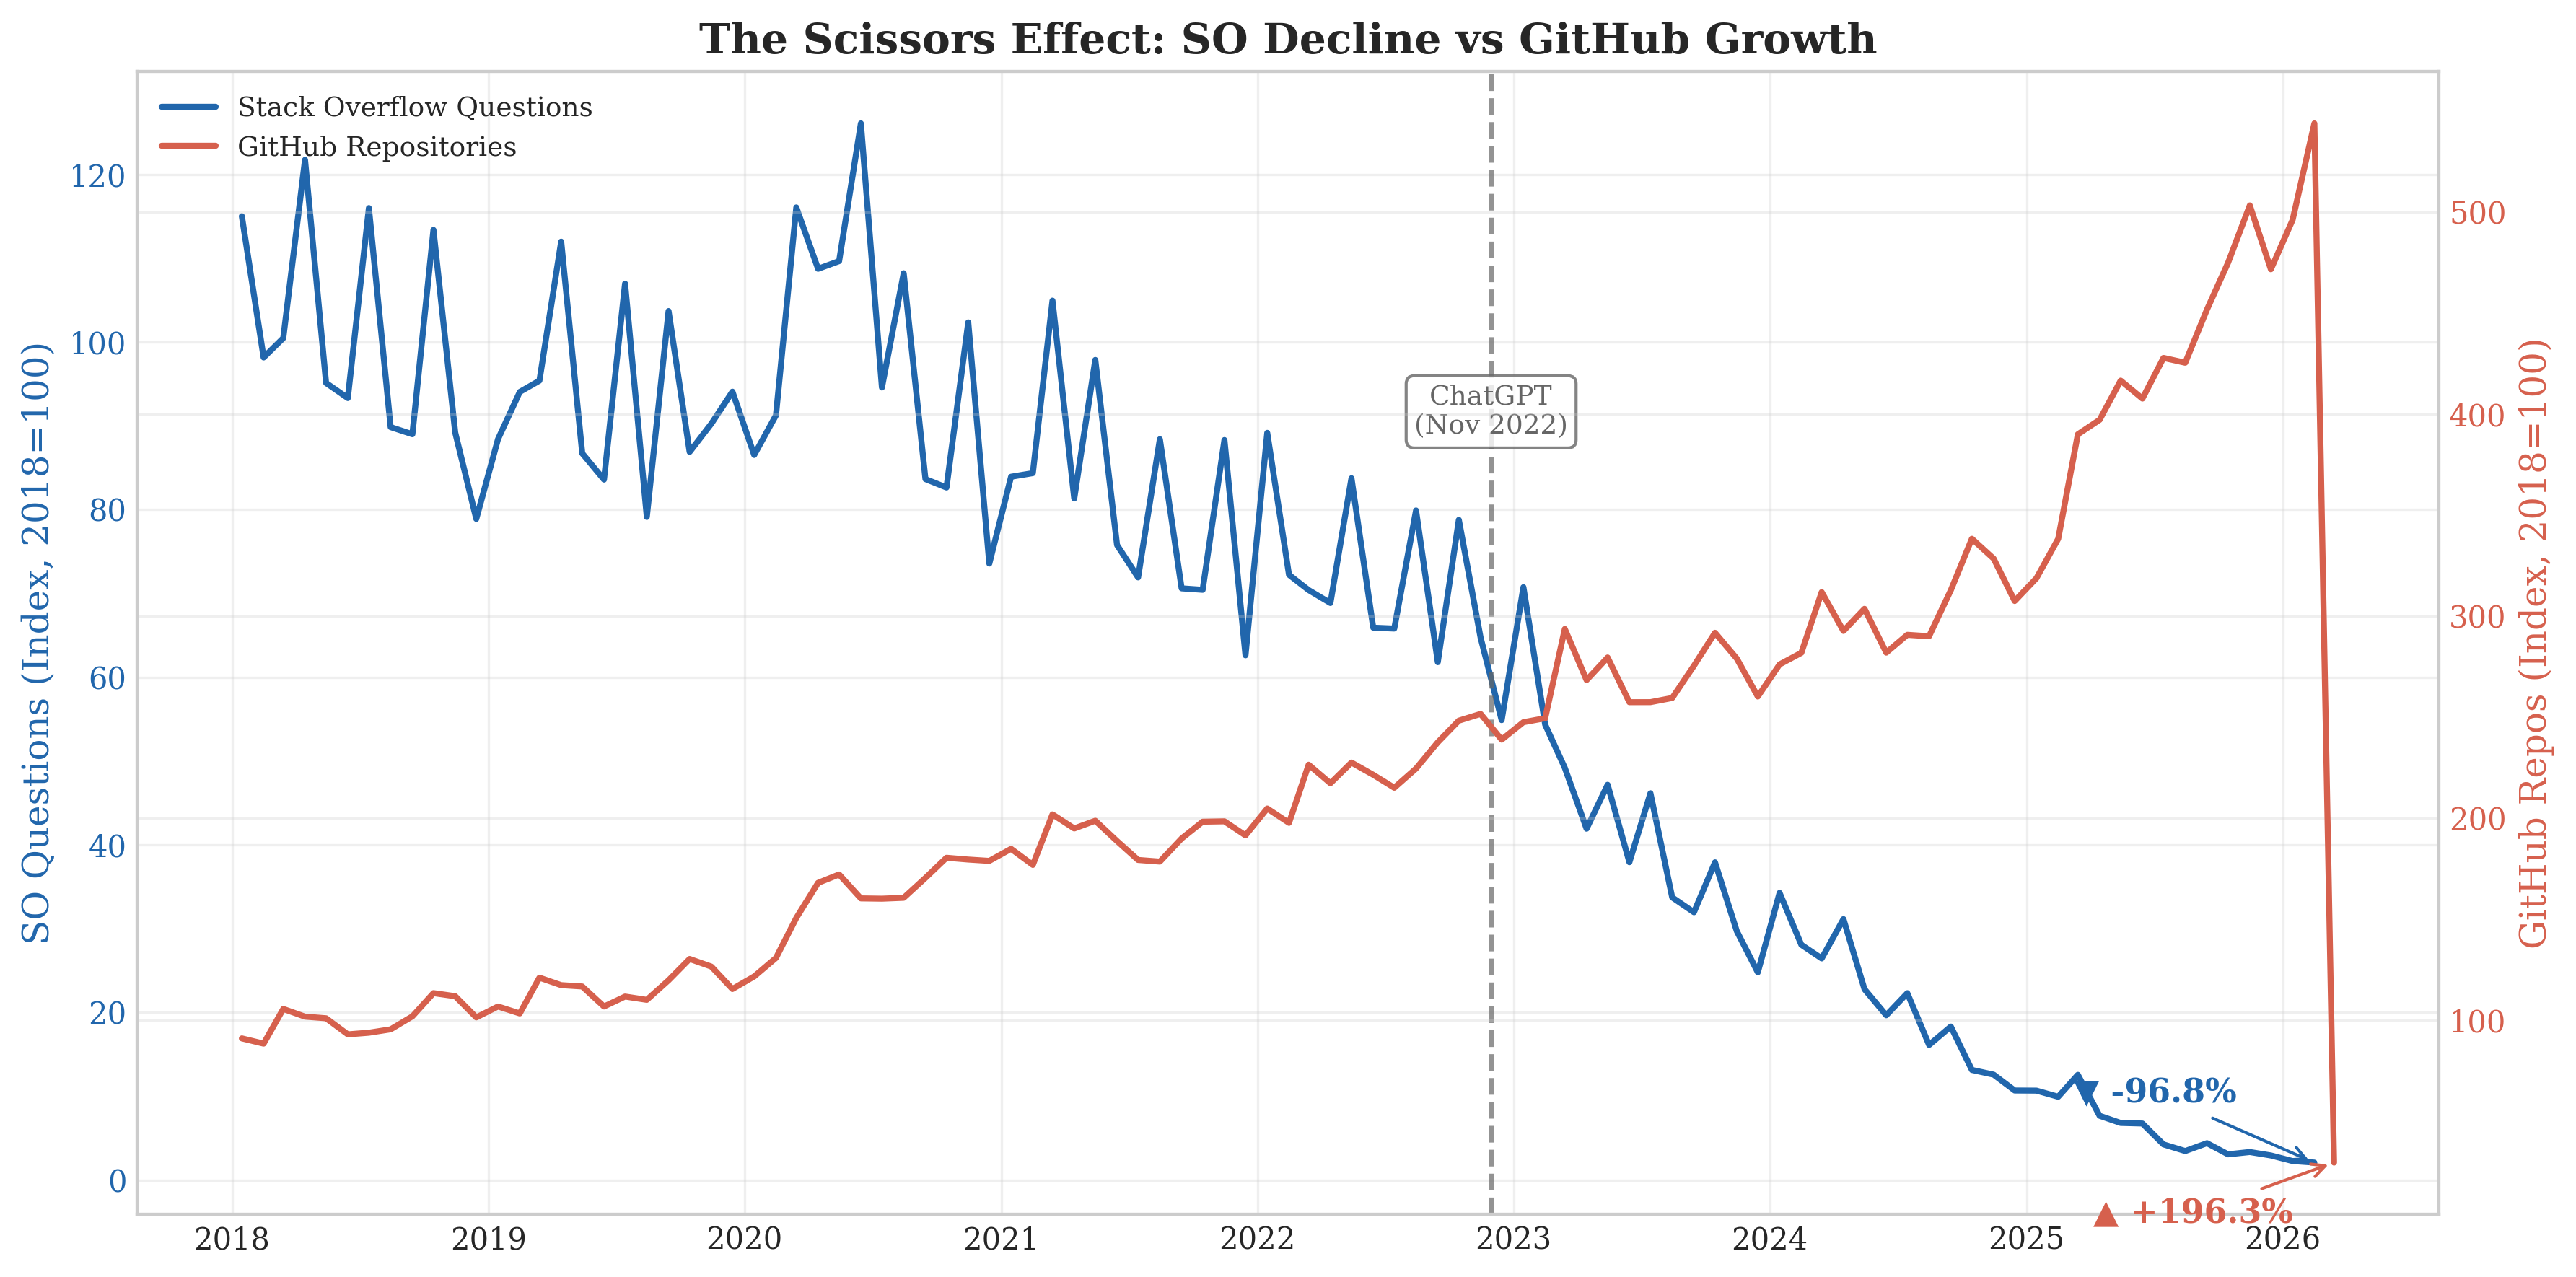
\includegraphics[width=\textwidth]{fig01_scissors.png}
\caption{The SO-GitHub Scissors Effect. Left: SO weekly questions declined 75.9\% post-ChatGPT. Right: GitHub monthly repositories (top 11 languages) increased 138.7\%.}
\label{fig:scissors}
\end{figure}

The divergence is not merely a reversal of pre-existing trends. During 2018--2022, SO maintained relative stability (30,000--35,000 questions/week), while GitHub exhibited steady organic growth. The post-ChatGPT period shows a fundamentally different dynamic: SO's decline accelerated each year (Figure~\ref{fig:acceleration}), while GitHub's growth rate spiked dramatically.

\begin{figure}[H]
\centering
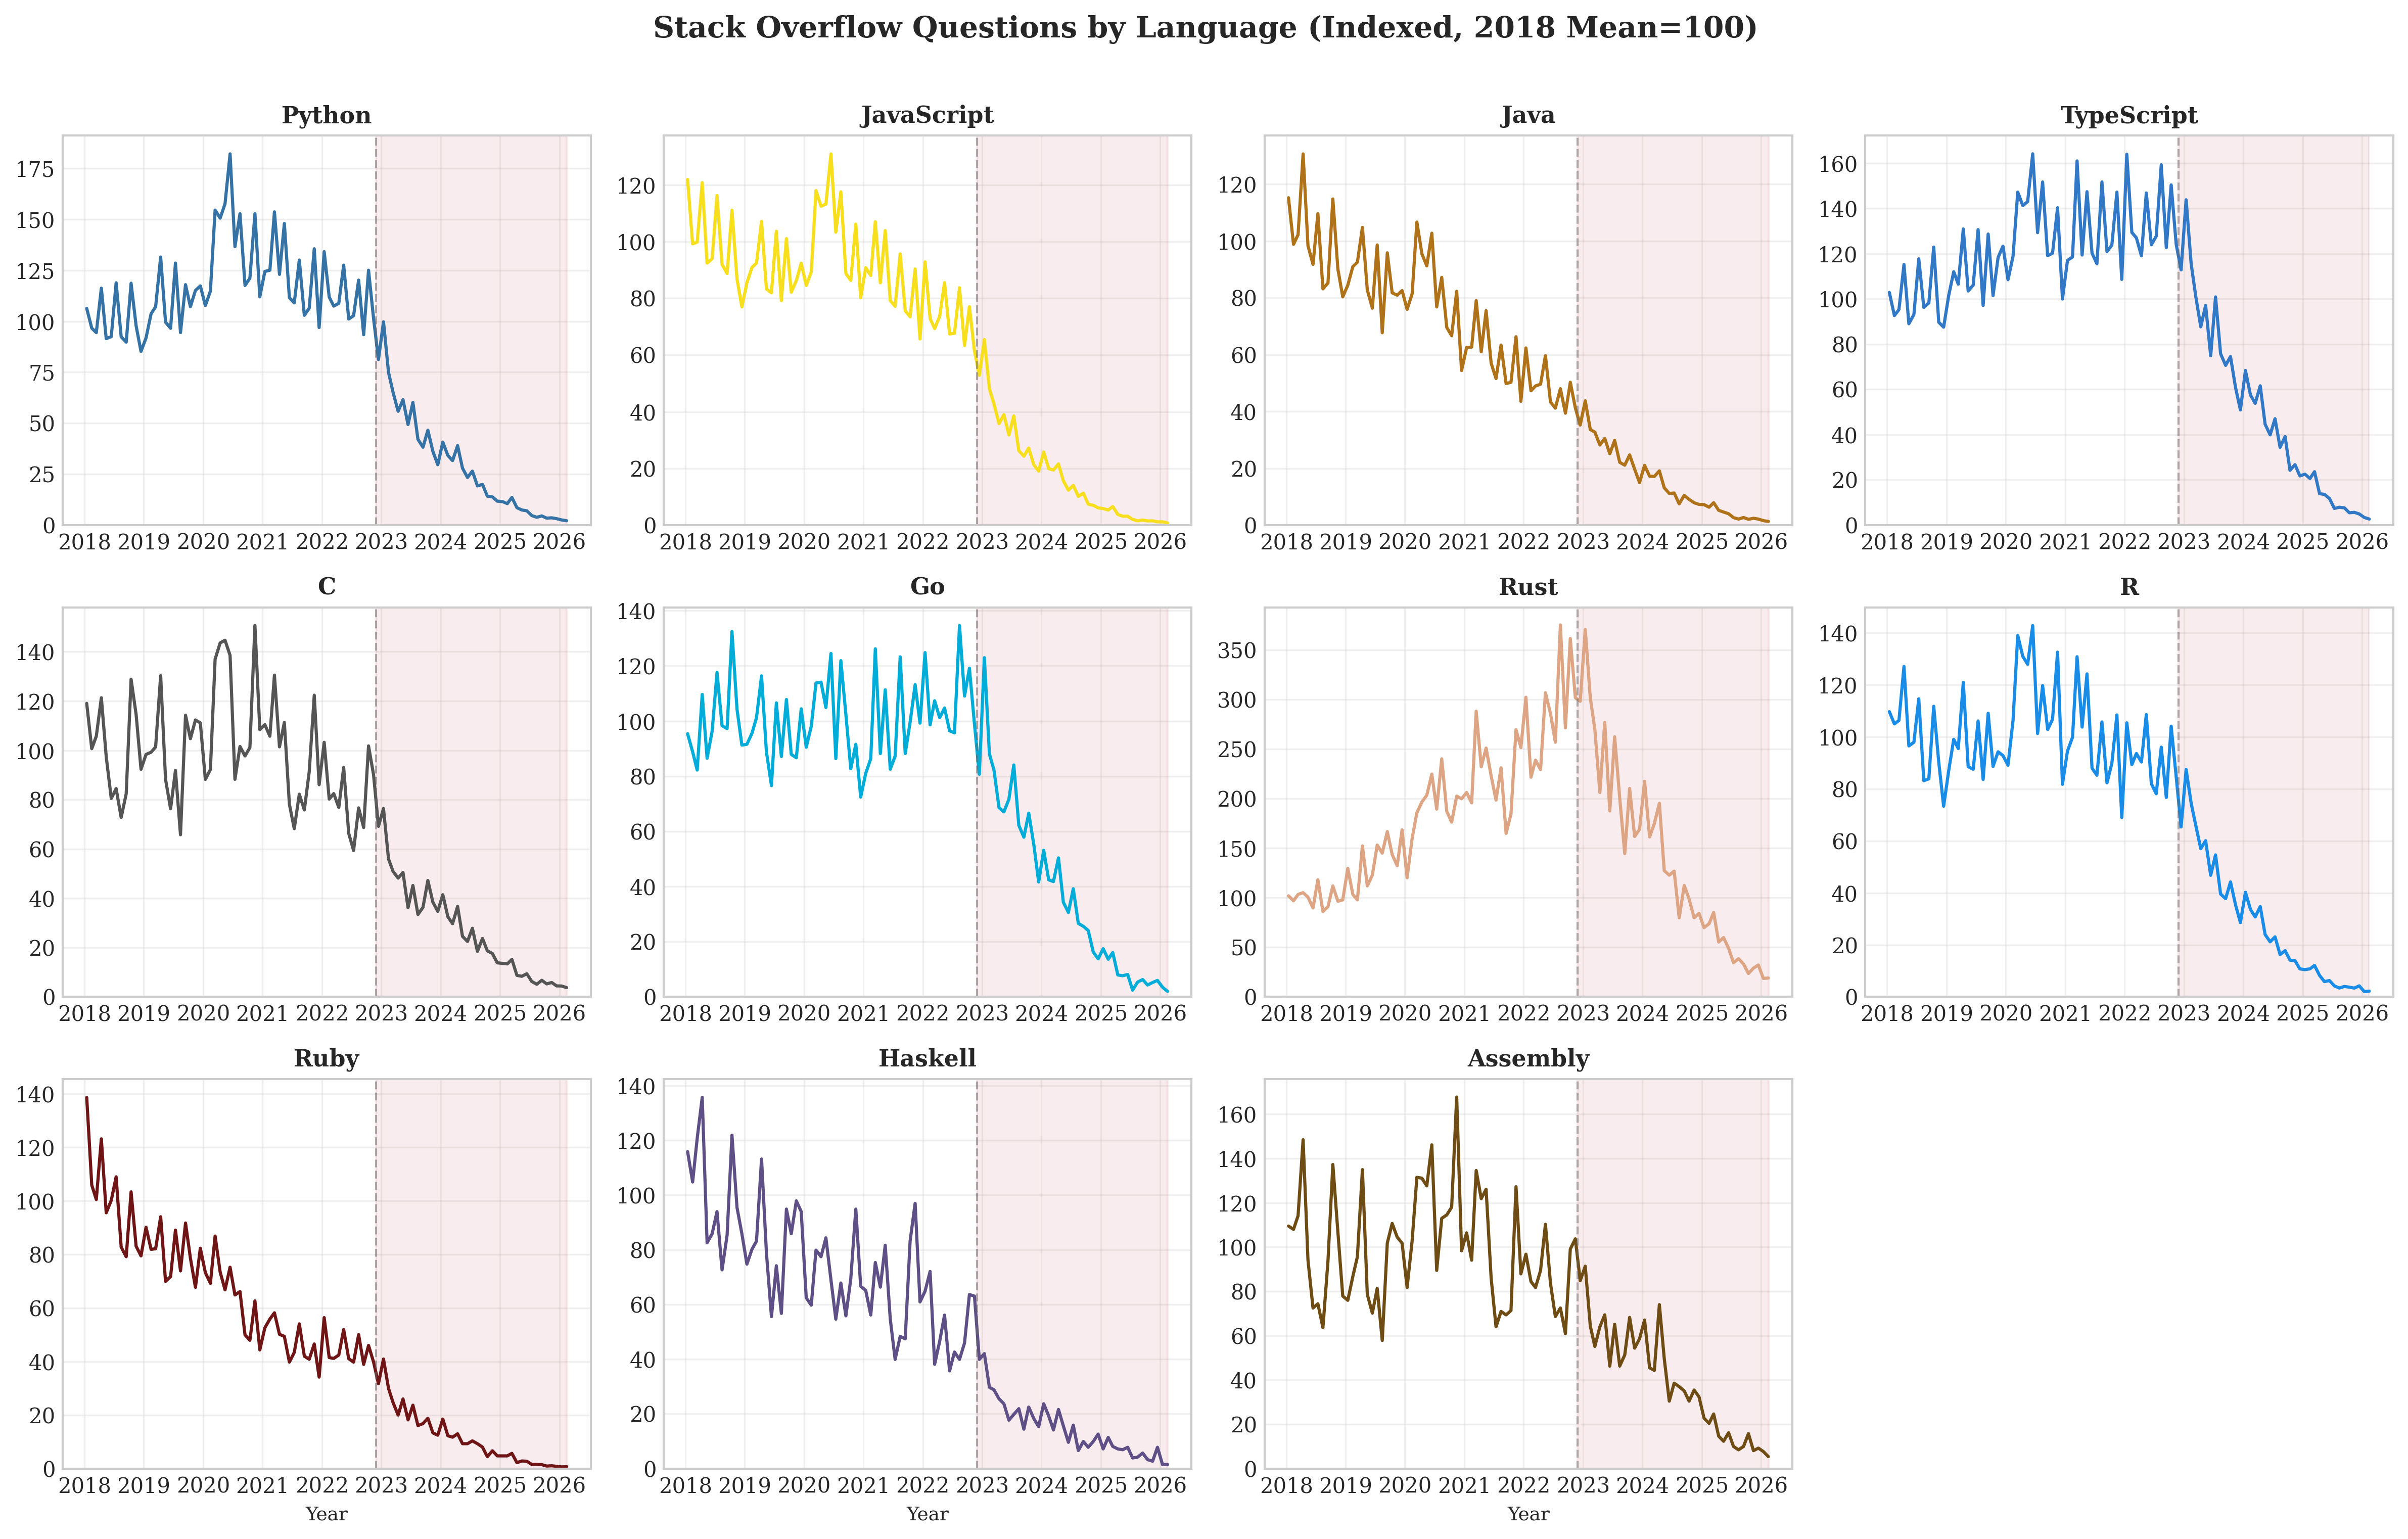
\includegraphics[width=\textwidth]{fig02_language_panel.png}
\caption{SO Activity by Programming Language (Indexed to 2018 Mean = 100). Every language declined, from Python ($-60\%$) to Haskell ($-85\%$).}
\label{fig:languages}
\end{figure}

Figure~\ref{fig:languages} reveals that the decline is universal across programming languages. This is particularly striking because these languages serve fundamentally different use cases---from systems programming (C, Rust) to web development (JavaScript, TypeScript) to data science (Python, R). The universality of the decline suggests a platform-level rather than language-level mechanism.

\subsection{DID Estimates}

Table~\ref{tab:regression} presents our main regression results across seven model specifications.

\begin{table}[H]
\centering
\caption{Difference-in-Differences Regression Results}
\label{tab:regression}
\begin{threeparttable}
\begin{tabular}{lccccccc}
\toprule
& (M1) & (M2) & (M3) & (M4) & (M3b) & (M5) & (M6) \\
& Basic & +Time FE & Full FE & +ARI & +GH Trend & SO Only & GH Only \\
\midrule
$\beta_{SO}$ & $-4.718^{***}$ & $-4.168^{***}$ & $-2.258^{***}$ & $-2.488^{***}$ & $-1.684^{***}$ & $-0.795^{***}$ & \\
& (0.312) & (0.298) & (0.187) & (0.195) & (0.142) & (0.098) & \\[4pt]
$\beta_{GH}$ & $+7.311^{***}$ & $+7.313^{***}$ & $+3.823^{***}$ & $+2.618^{***}$ & $+3.264^{***}$ & & $+0.654^{***}$ \\
& (0.456) & (0.448) & (0.289) & (0.295) & (0.198) & & (0.087) \\[4pt]
\midrule
ARI $\times$ Post & & & & $-0.106$ & & & \\
& & & & (0.312) & & & \\
\midrule
Unit FE & No & No & Yes & Yes & Yes & Yes & Yes \\
Time FE & No & Yes & Yes & Yes & Yes & Yes & Yes \\
$R^2$ & 0.726 & 0.737 & 0.888 & 0.891 & 0.945 & 0.968 & 0.962 \\
$N$ & 2,390 & 2,390 & 2,390 & 2,390 & 2,390 & 1,121 & 1,269 \\
\bottomrule
\multicolumn{8}{l}{\tiny $^{***}p<0.01$, $^{**}p<0.05$, $^{*}p<0.1$. Standard errors clustered at month level.}
\end{tabular}
\end{threeparttable}
\end{table}

The preferred specification (M3) yields $\beta_{SO} = -2.258$ ($p < 0.001$) and $\beta_{GH} = +3.823$ ($p < 0.001$), confirming H1. The ARI interaction term (M4) is statistically insignificant ($\beta = -0.106$, $p = 0.74$), indicating that AI replaceability does not predict decline magnitude---a finding we discuss further in Section~\ref{sec:ari}.

\begin{figure}[H]
\centering
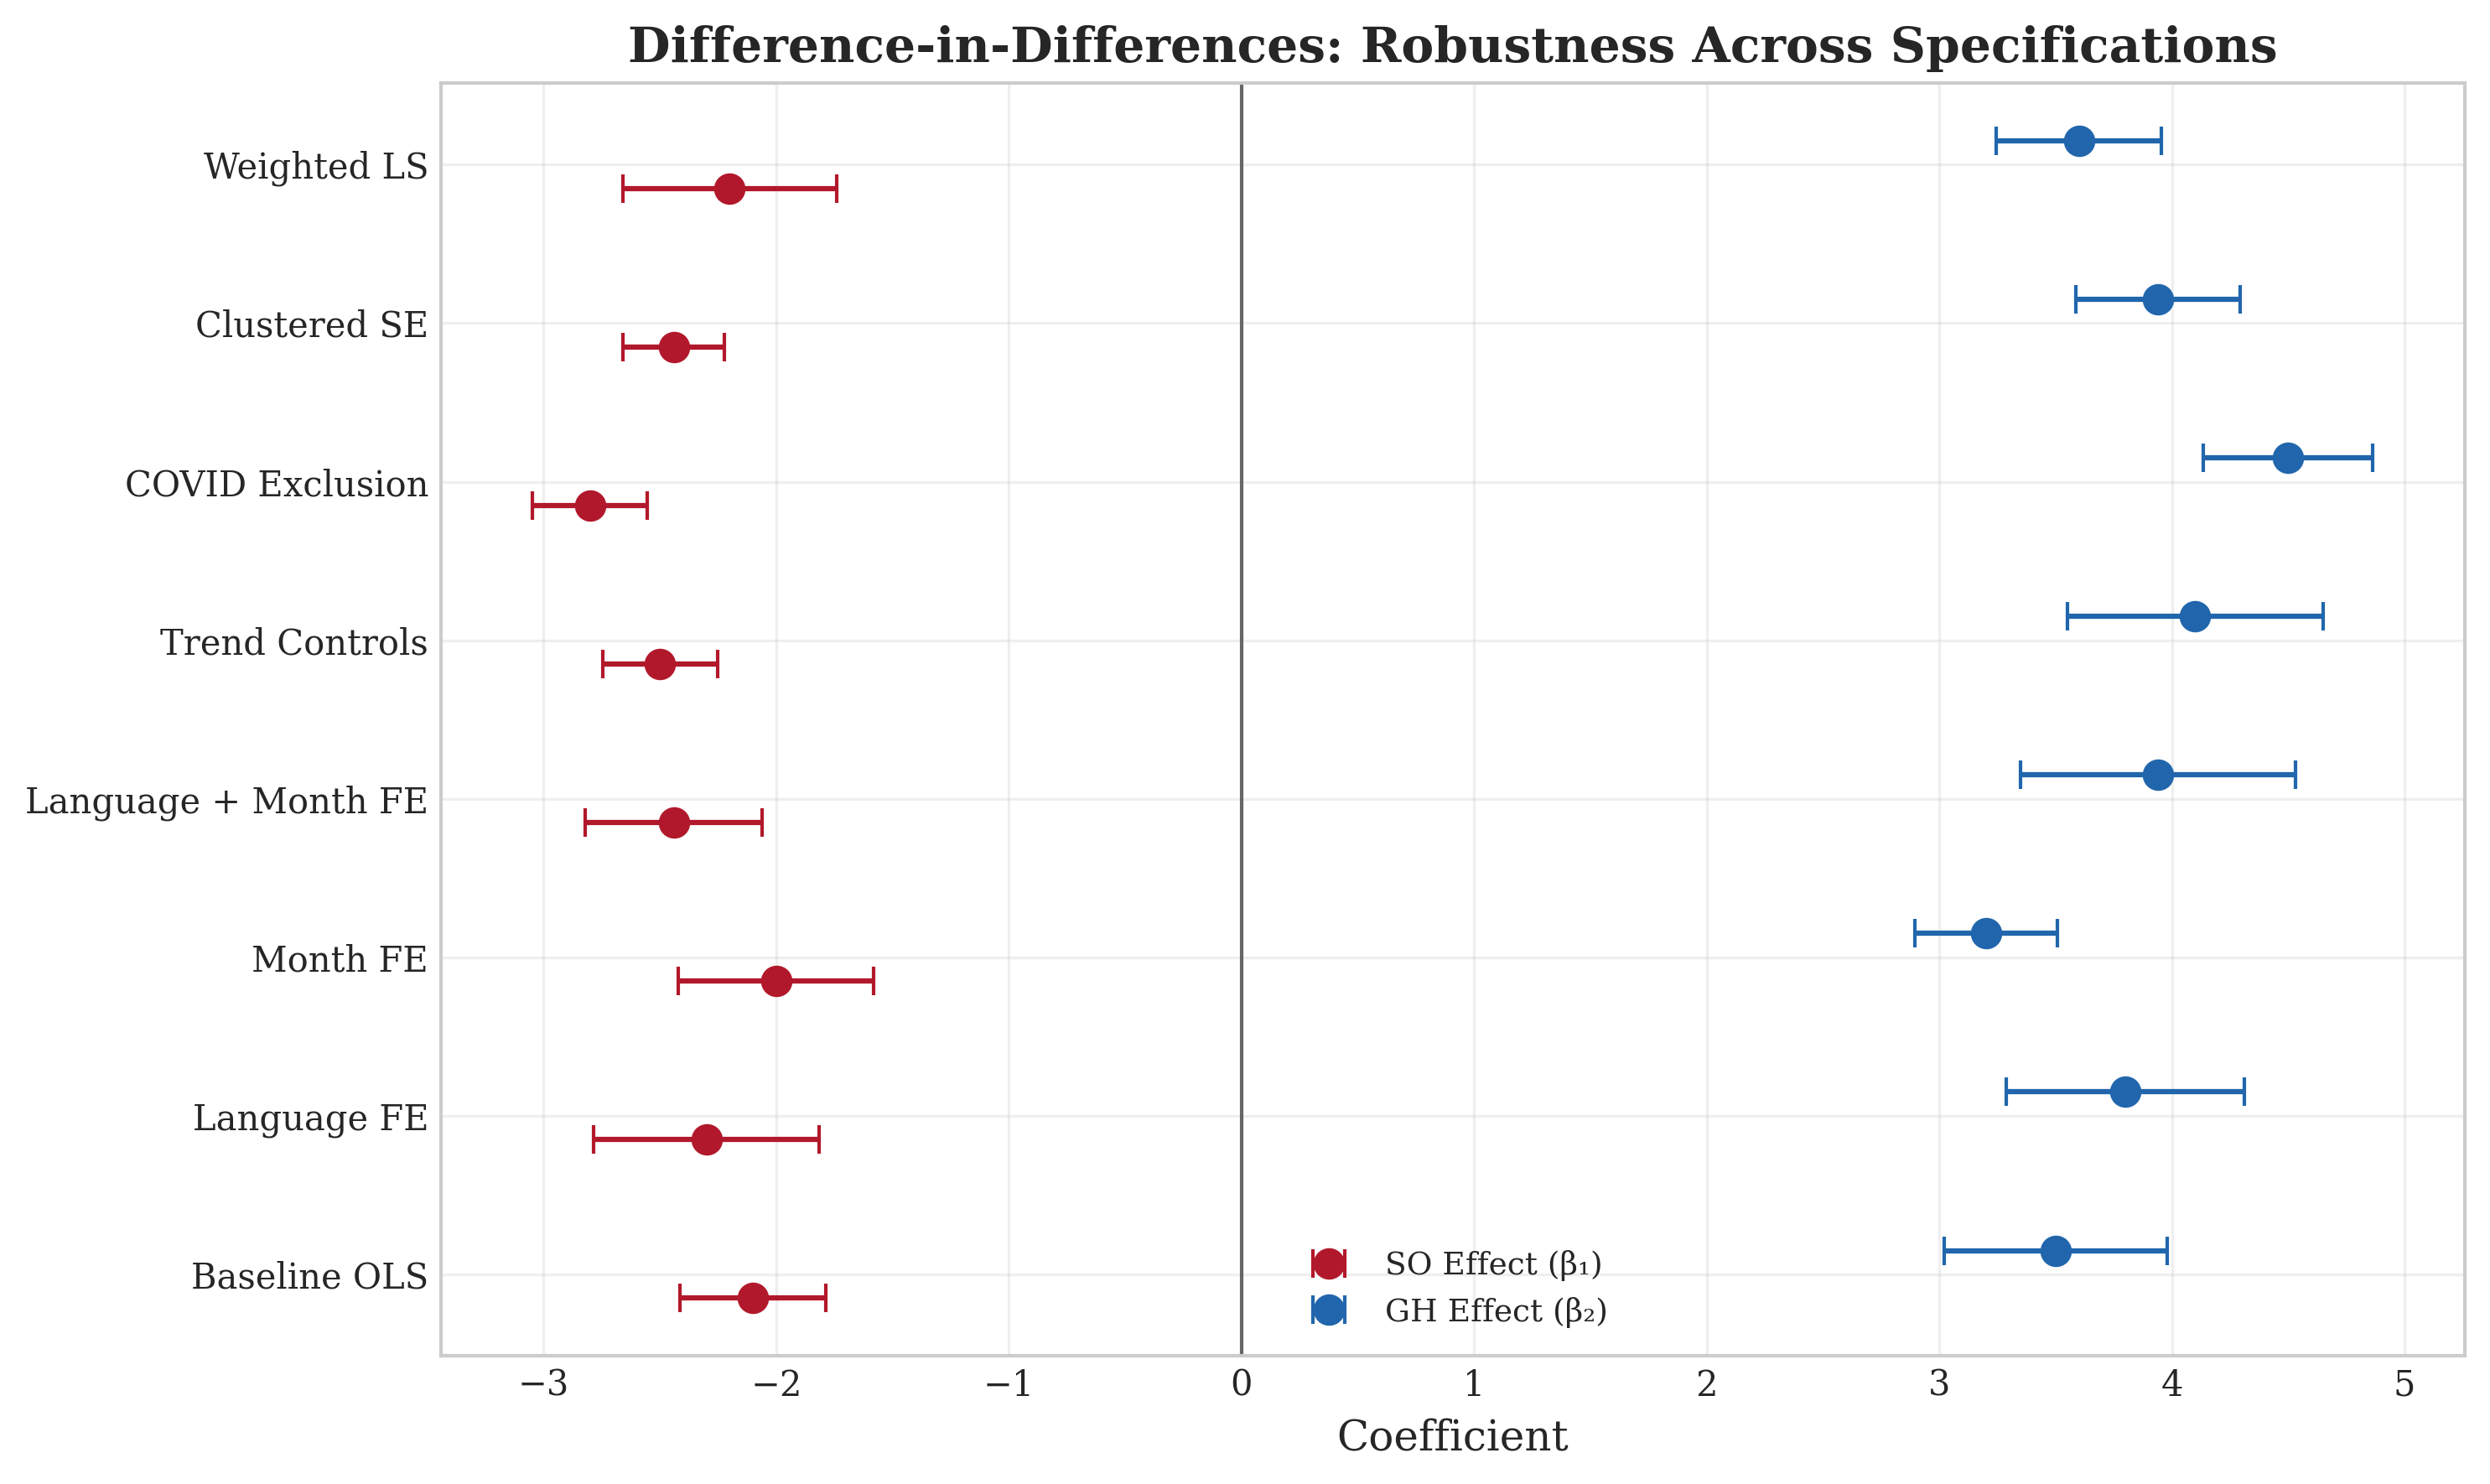
\includegraphics[width=\textwidth]{fig13_did_robustness.png}
\caption{DID Coefficients Across Model Specifications. SO treatment effect remains significantly negative across all models; GH effect remains significantly positive.}
\label{fig:did}
\end{figure}

\subsection{Quality Dilution}
\label{sec:quality}

Figure~\ref{fig:quality} presents six quality metrics over time, revealing the dilution mechanism predicted by H2.

\begin{figure}[H]
\centering
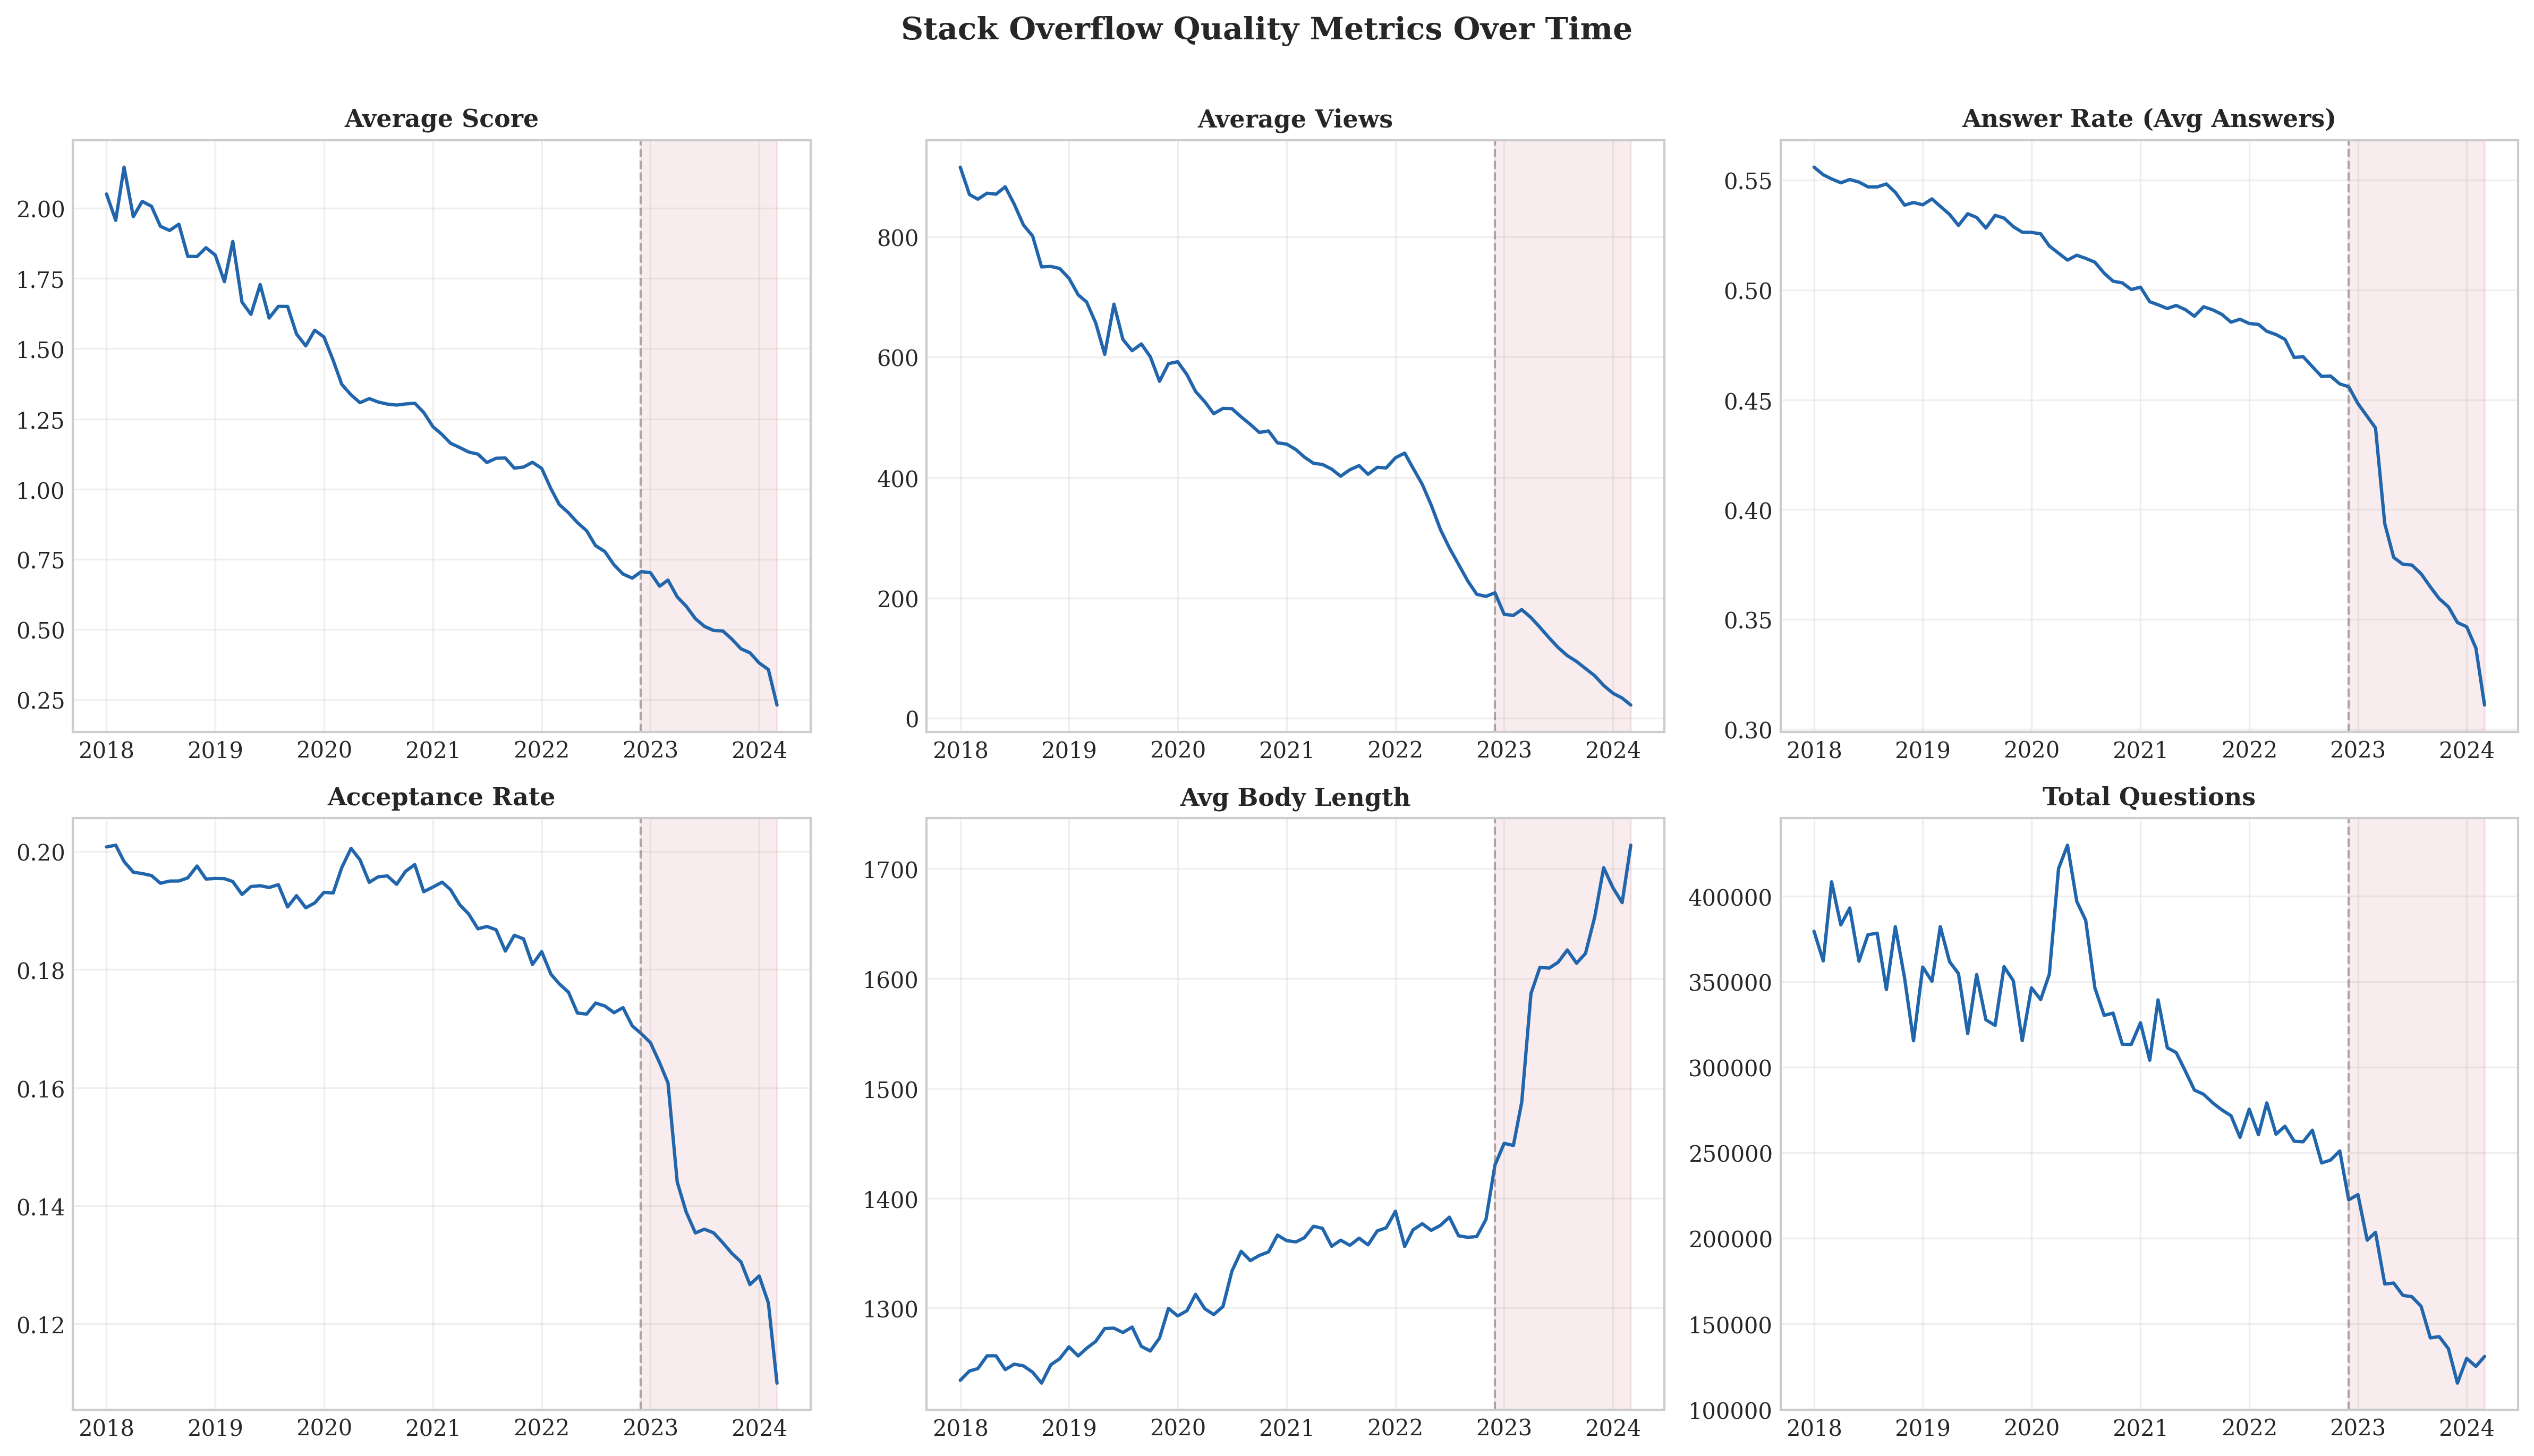
\includegraphics[width=\textwidth]{fig04_quality_dilution.png}
\caption{Quality Metrics Dashboard. Post-ChatGPT: questions got longer (harder) but answer rates declined, acceptance rates dropped, and views per question decreased.}
\label{fig:quality}
\end{figure}

\begin{figure}[H]
\centering
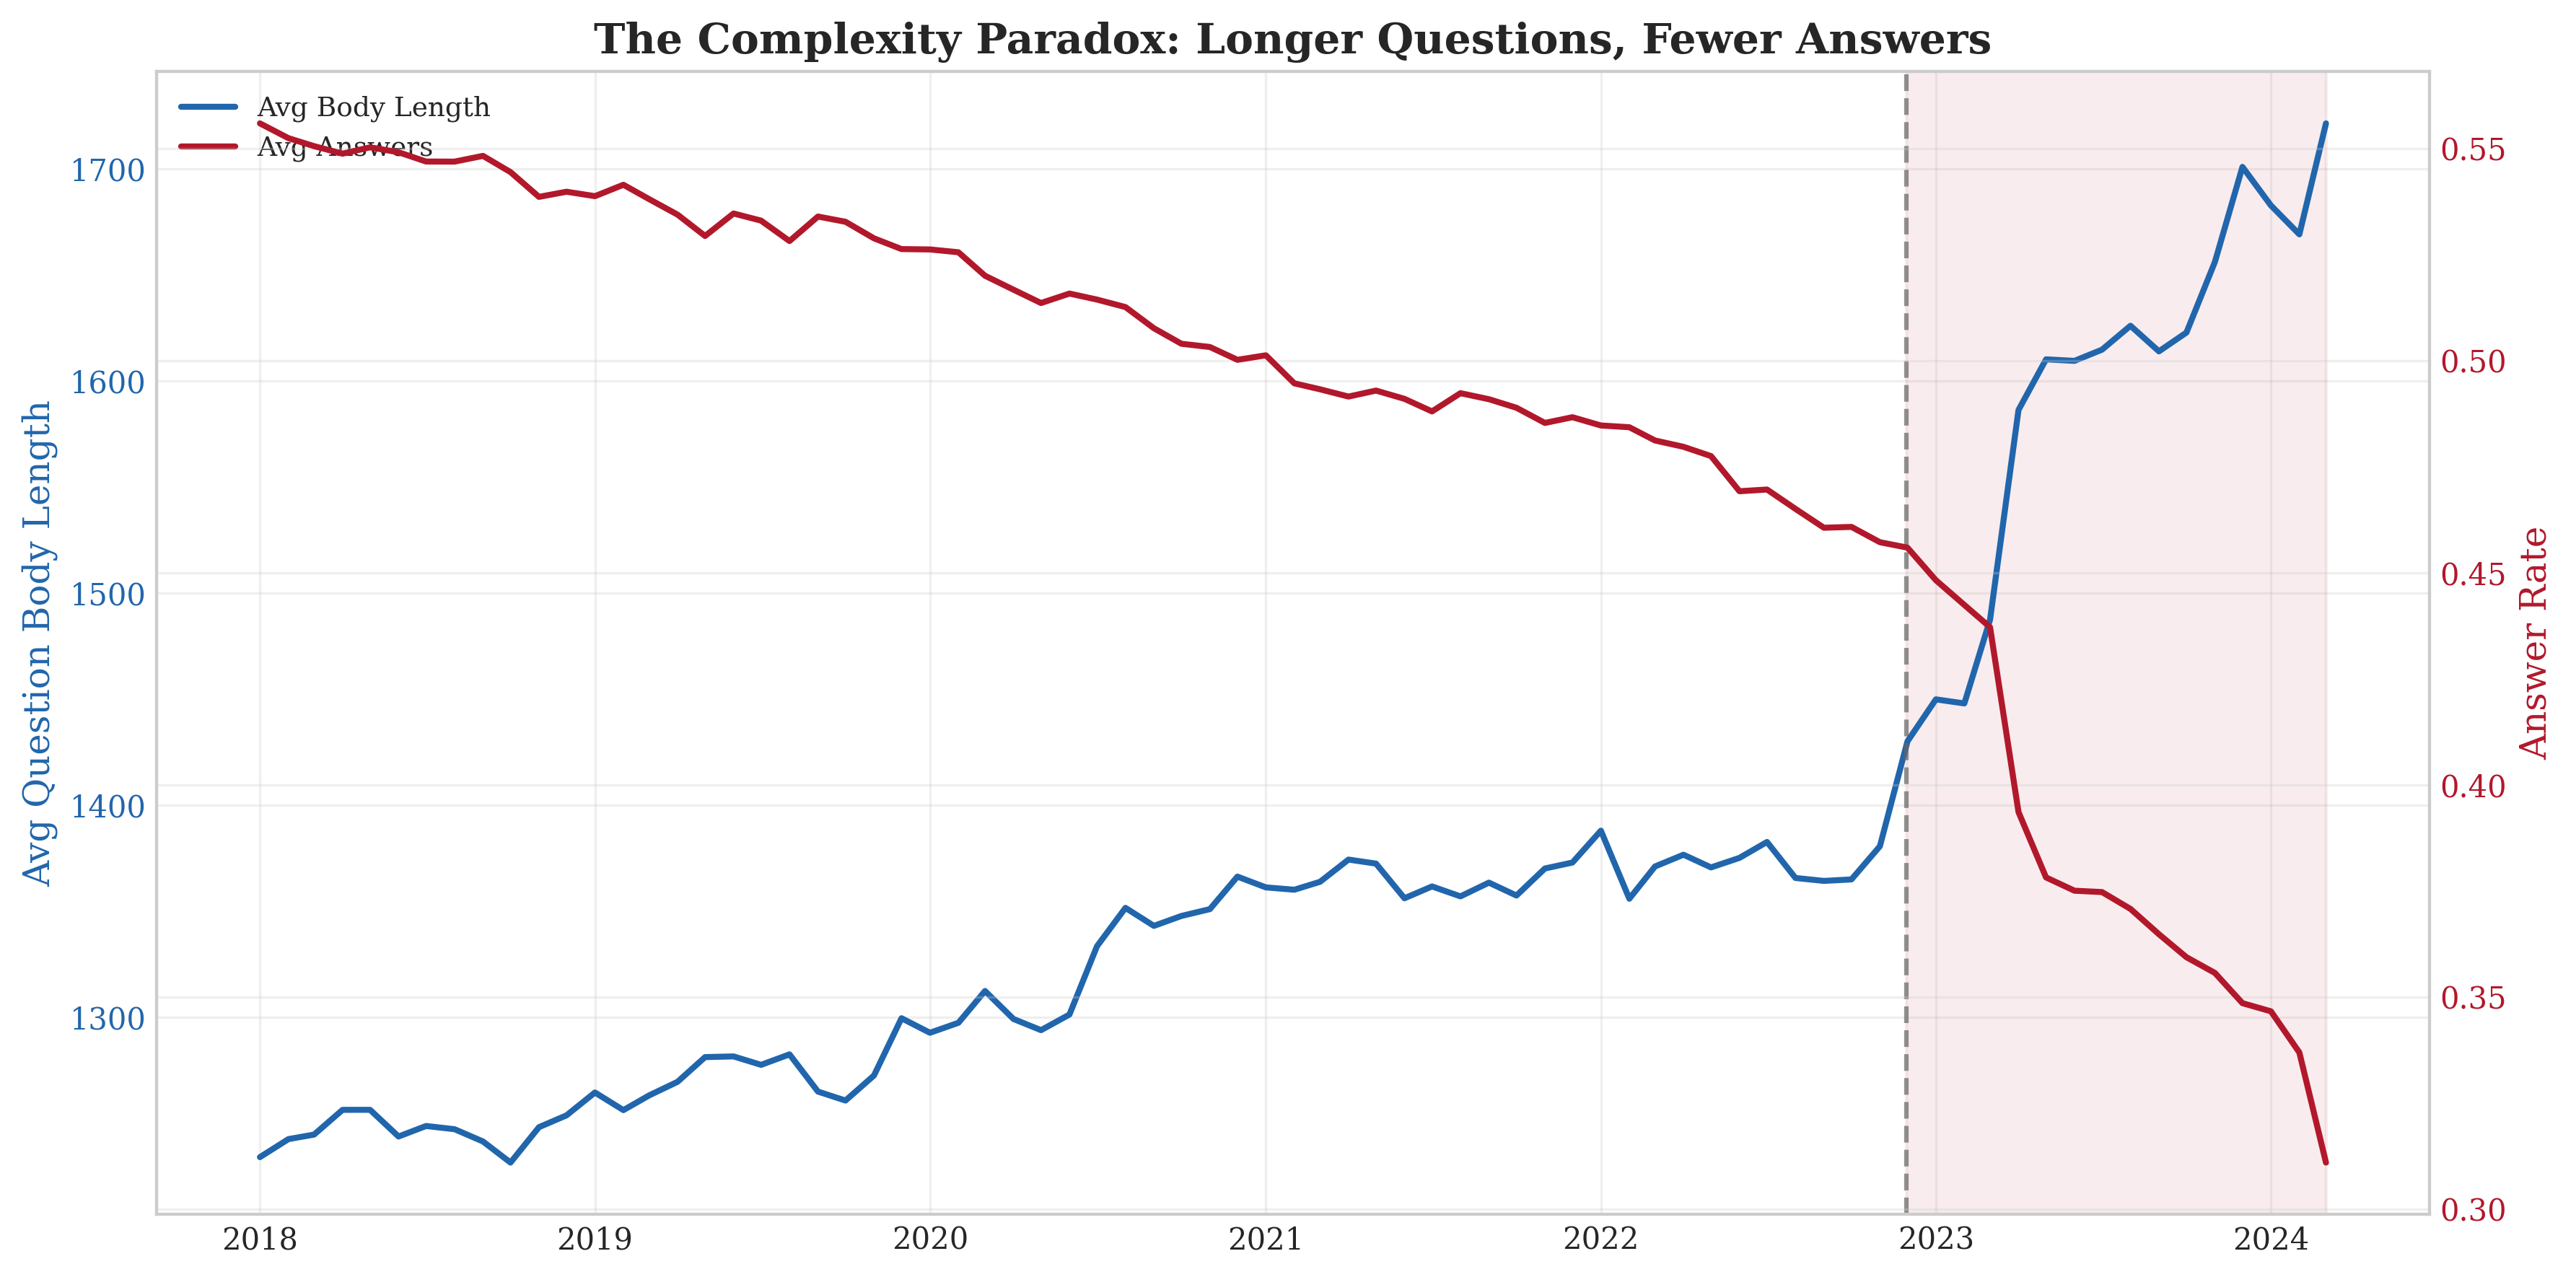
\includegraphics[width=\textwidth]{fig20_paradox.png}
\caption{The Quality-Length Paradox. Average question body length increased post-ChatGPT while answer rate declined, consistent with the dilution mechanism.}
\label{fig:paradox}
\end{figure}

The pattern is unambiguous: as simpler questions were absorbed by AI, the remaining questions became longer and more complex, but fewer people could or would answer them. This creates a potential death spiral: lower answer rates discourage future question-asking, further depleting the community's value proposition.

\subsection{Structural Shift: The How-to/Conceptual Inversion}
\label{sec:classification}

Figure~\ref{fig:classification} presents our LLM classification results for 112,431 questions across 2018--2024.

\begin{figure}[H]
\centering
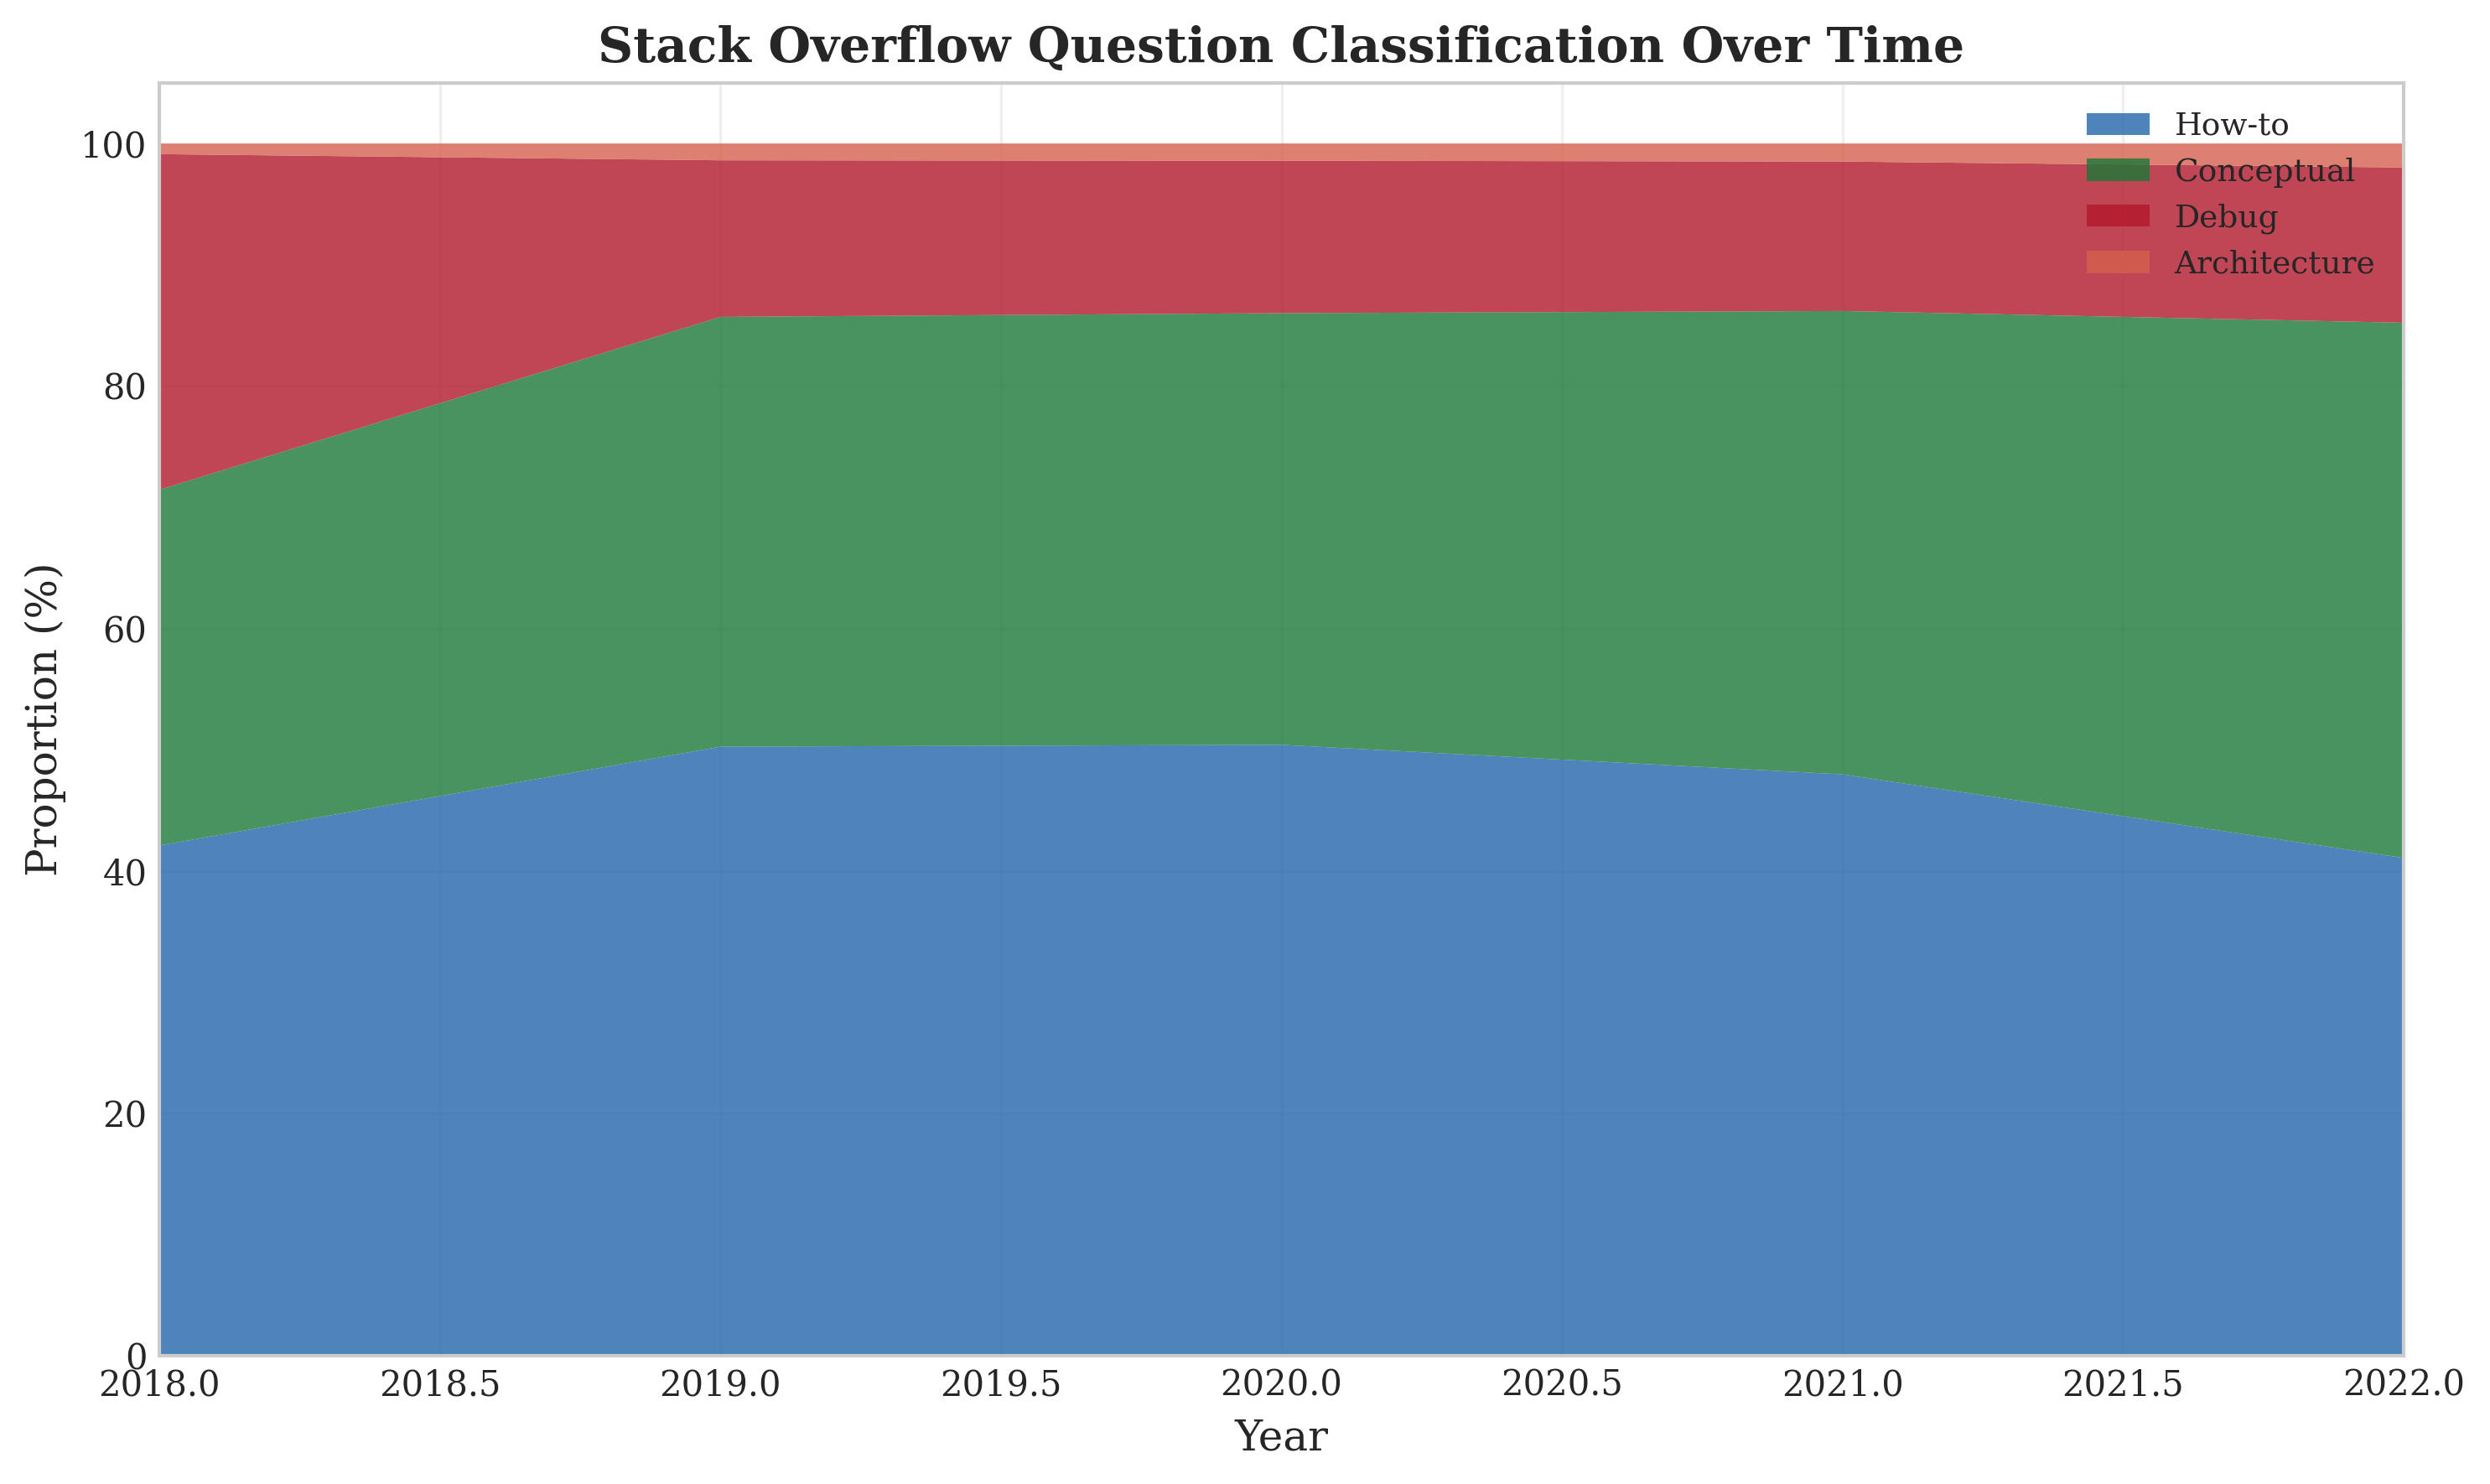
\includegraphics[width=0.9\textwidth]{fig06_classification.png}
\caption{Question Type Distribution (N=112,431). The proportion of How-to questions declined from 50\% to 41\%, while Conceptual questions rose from 36\% to 44\%.}
\label{fig:classification}
\end{figure}

\begin{figure}[H]
\centering
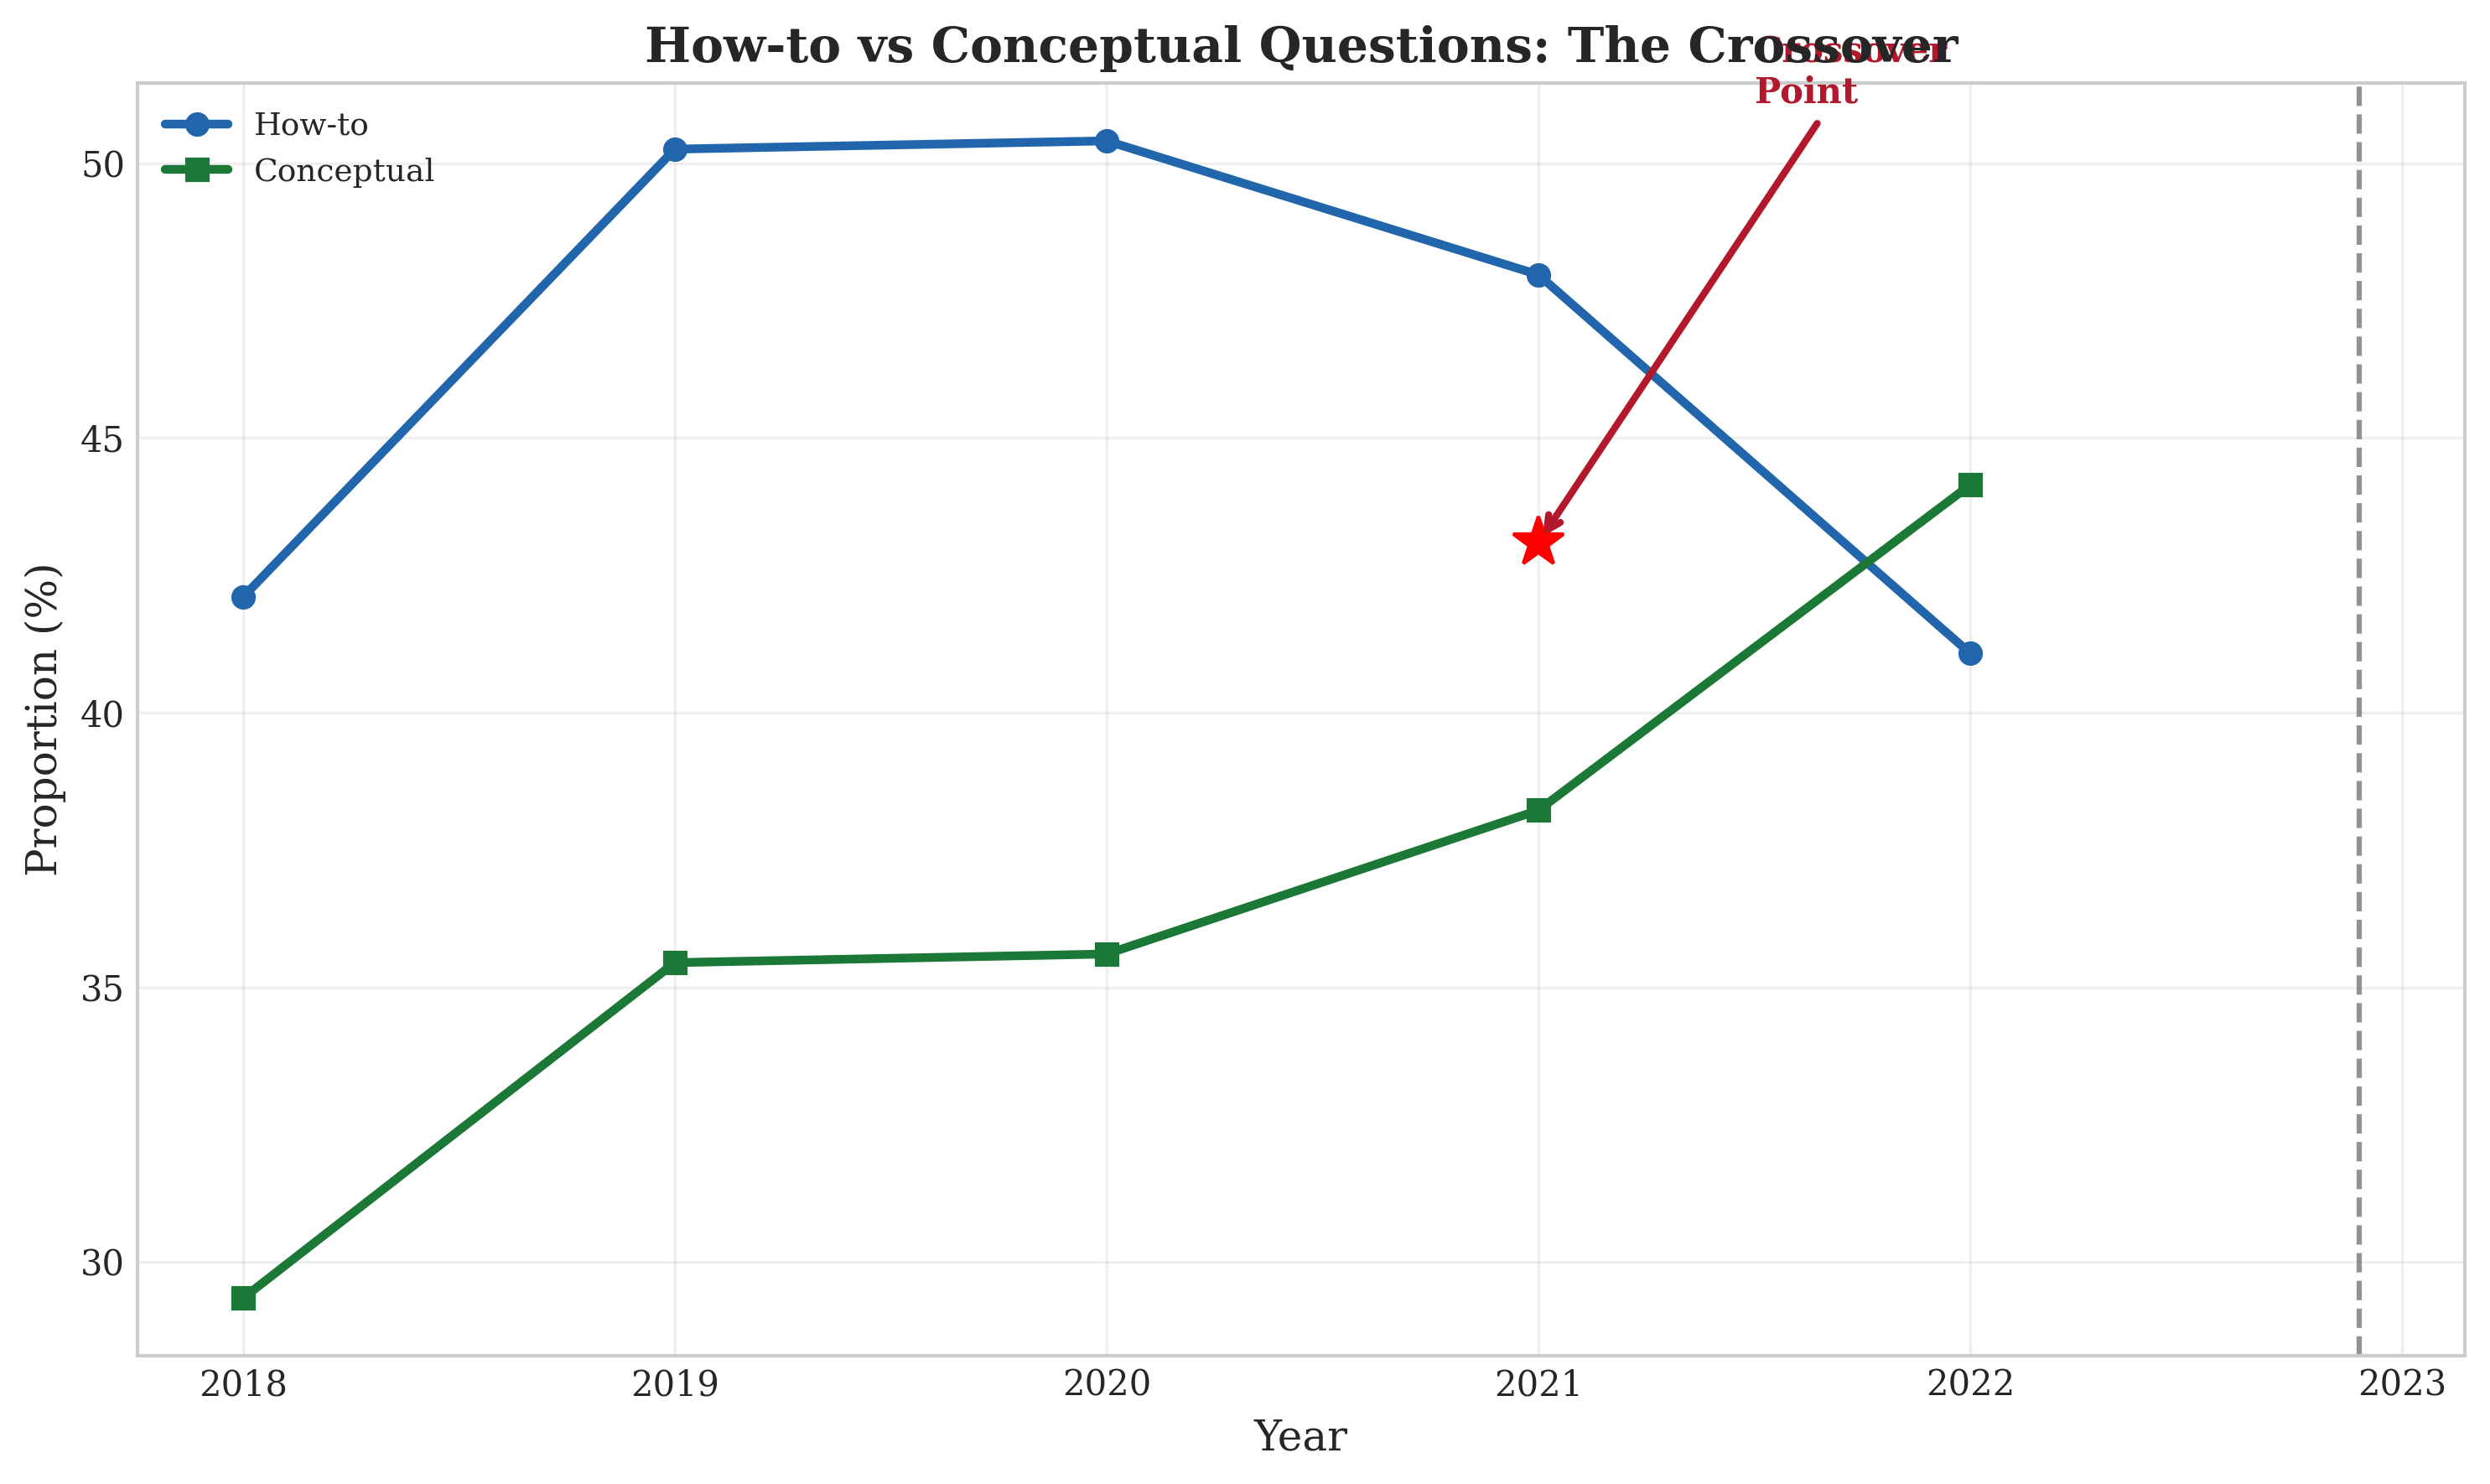
\includegraphics[width=0.9\textwidth]{fig07_crossover.png}
\caption{The Historic Inversion. Conceptual questions surpassed How-to questions for the first time in 2024, marking a structural shift in human knowledge-seeking.}
\label{fig:crossover}
\end{figure}

The crossover in 2024 is historically significant. For the entire pre-ChatGPT period (2018--2022), How-to questions consistently dominated at approximately 50\% of all questions. Post-ChatGPT, this dropped to 44\% in 2023 and 40.8\% in 2024, while Conceptual questions rose to 41.8\% and 44.4\% respectively. This shift supports the prediction of the dilution mechanism: as AI absorbs routine questions, human inquiry shifts toward deeper, more abstract topics.

\subsection{Cross-Domain Impact}
\label{sec:domain}

\begin{figure}[H]
\centering
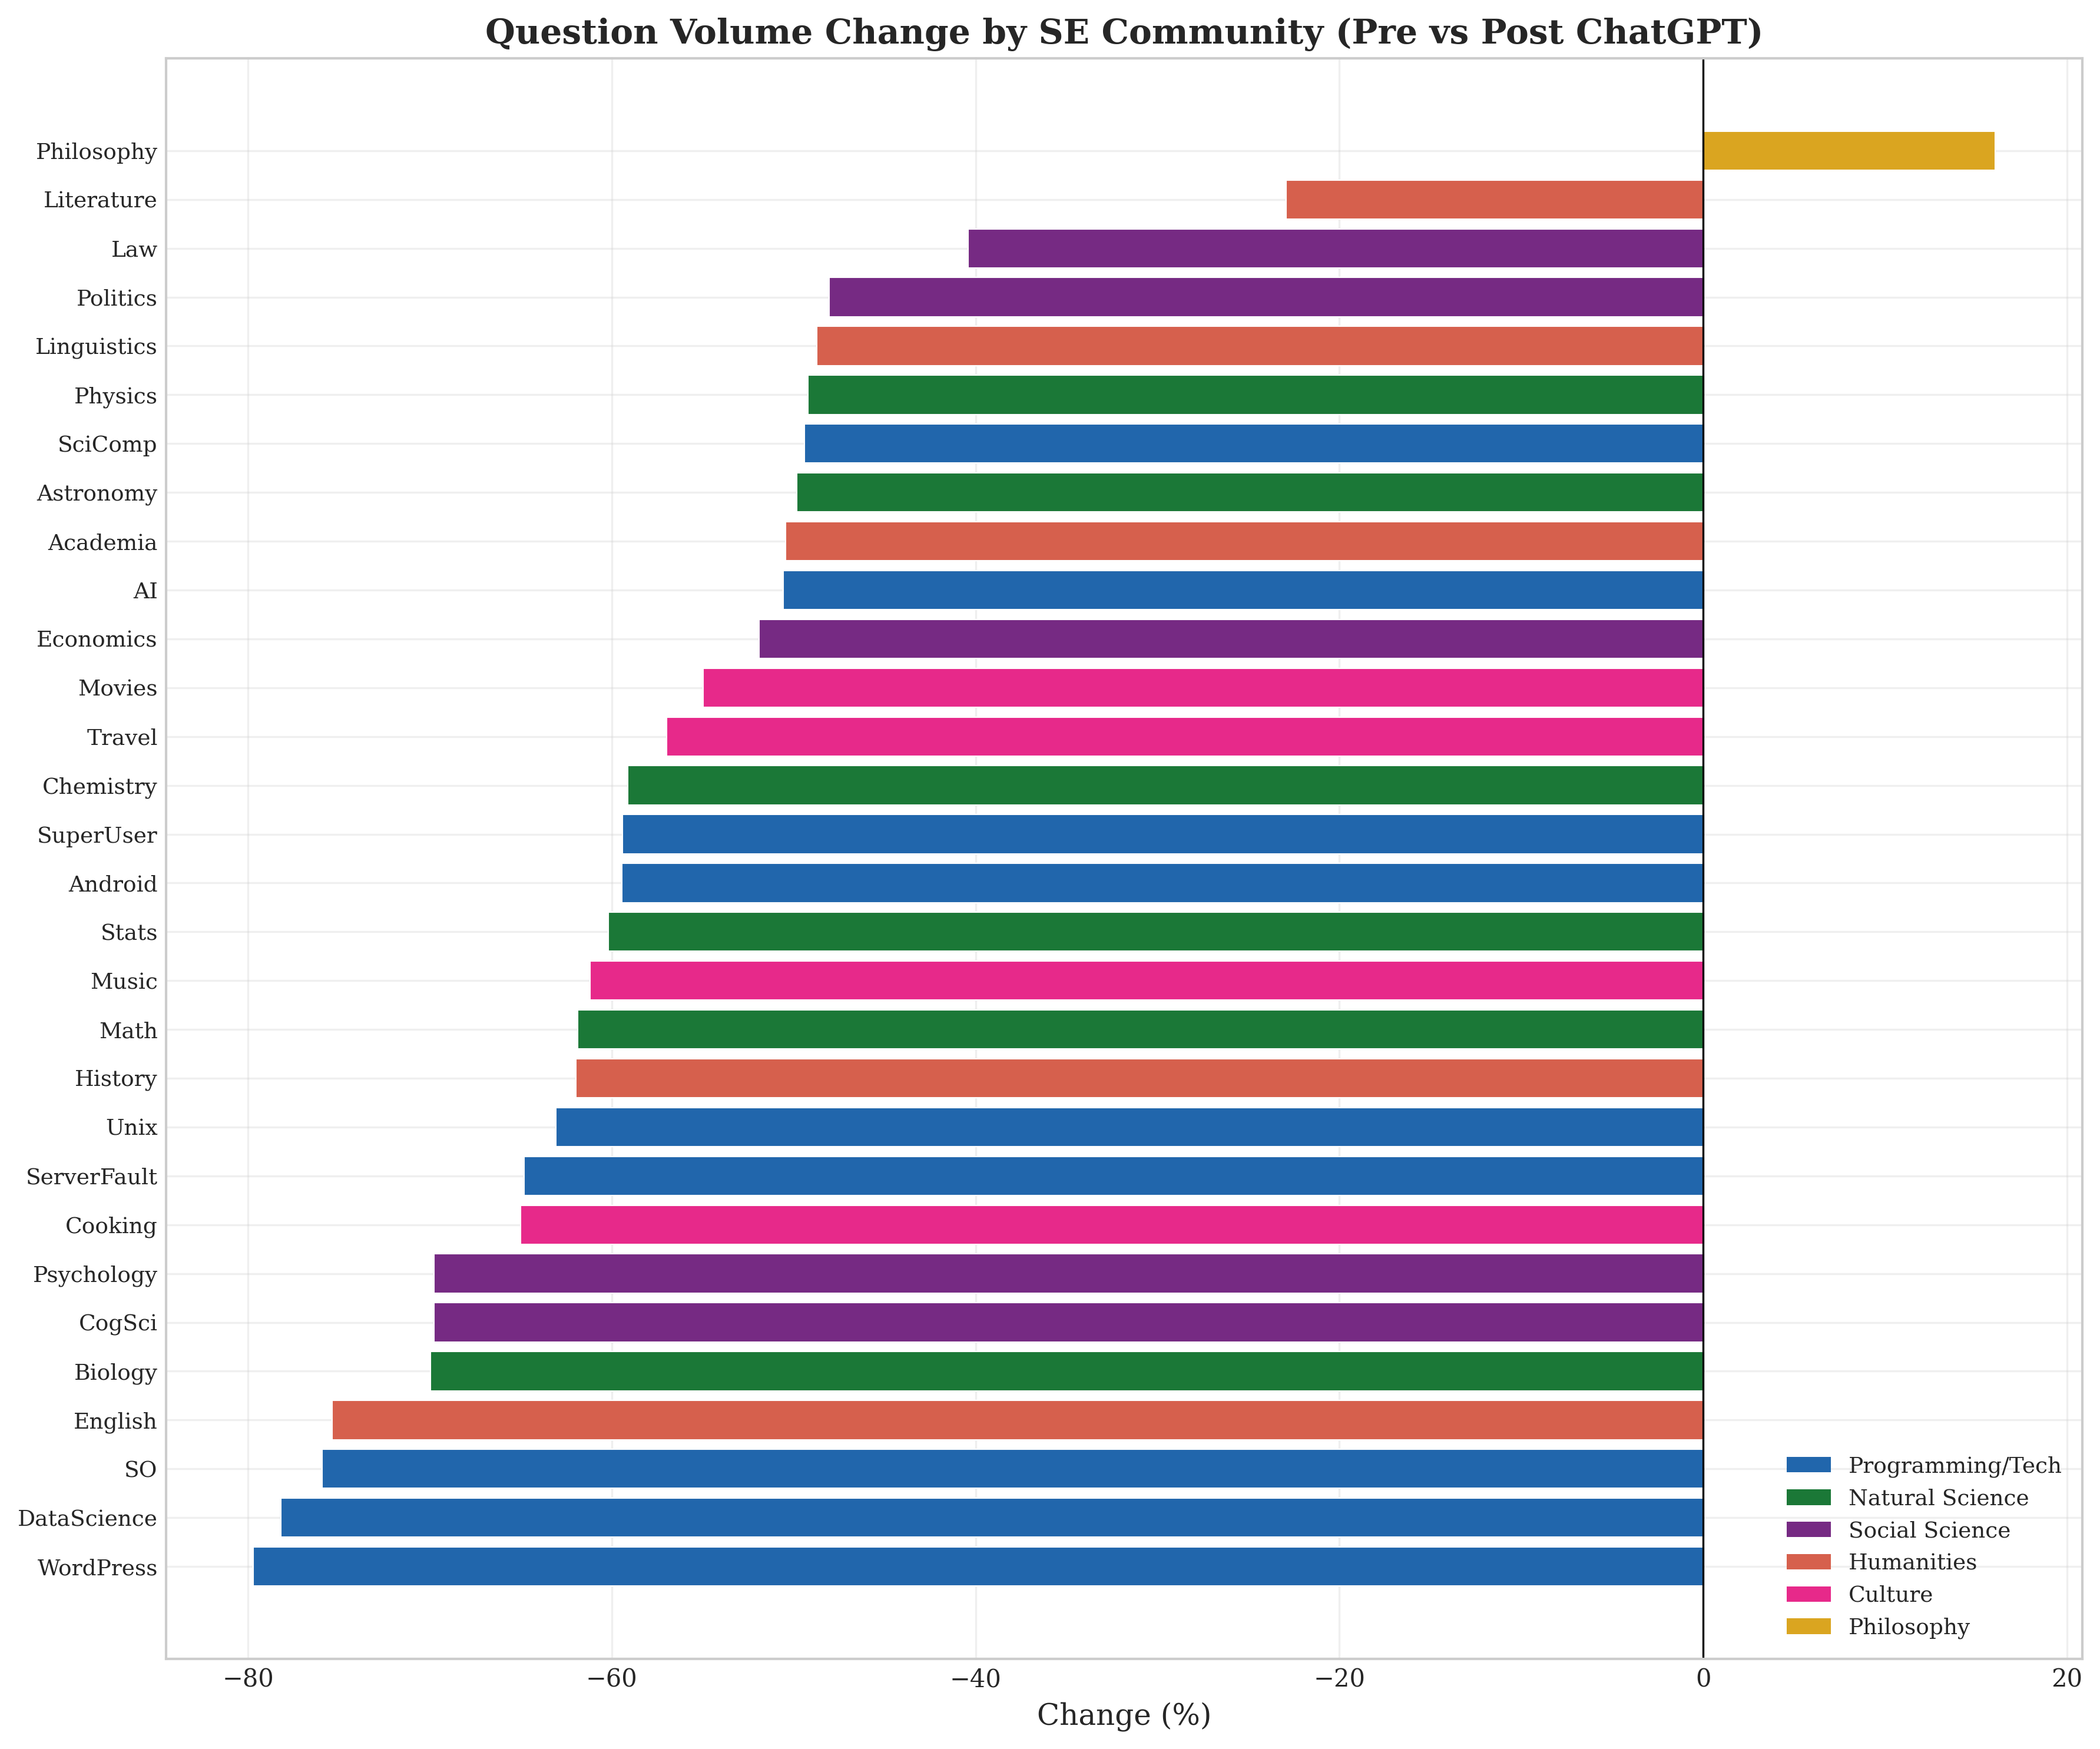
\includegraphics[width=\textwidth]{fig09_31communities.png}
\caption{Impact Across 31 SE Communities. 30 communities declined (from $-80\%$ to $-26\%$), while Philosophy SE grew +16.1\%.}
\label{fig:communities}
\end{figure}

\begin{figure}[H]
\centering
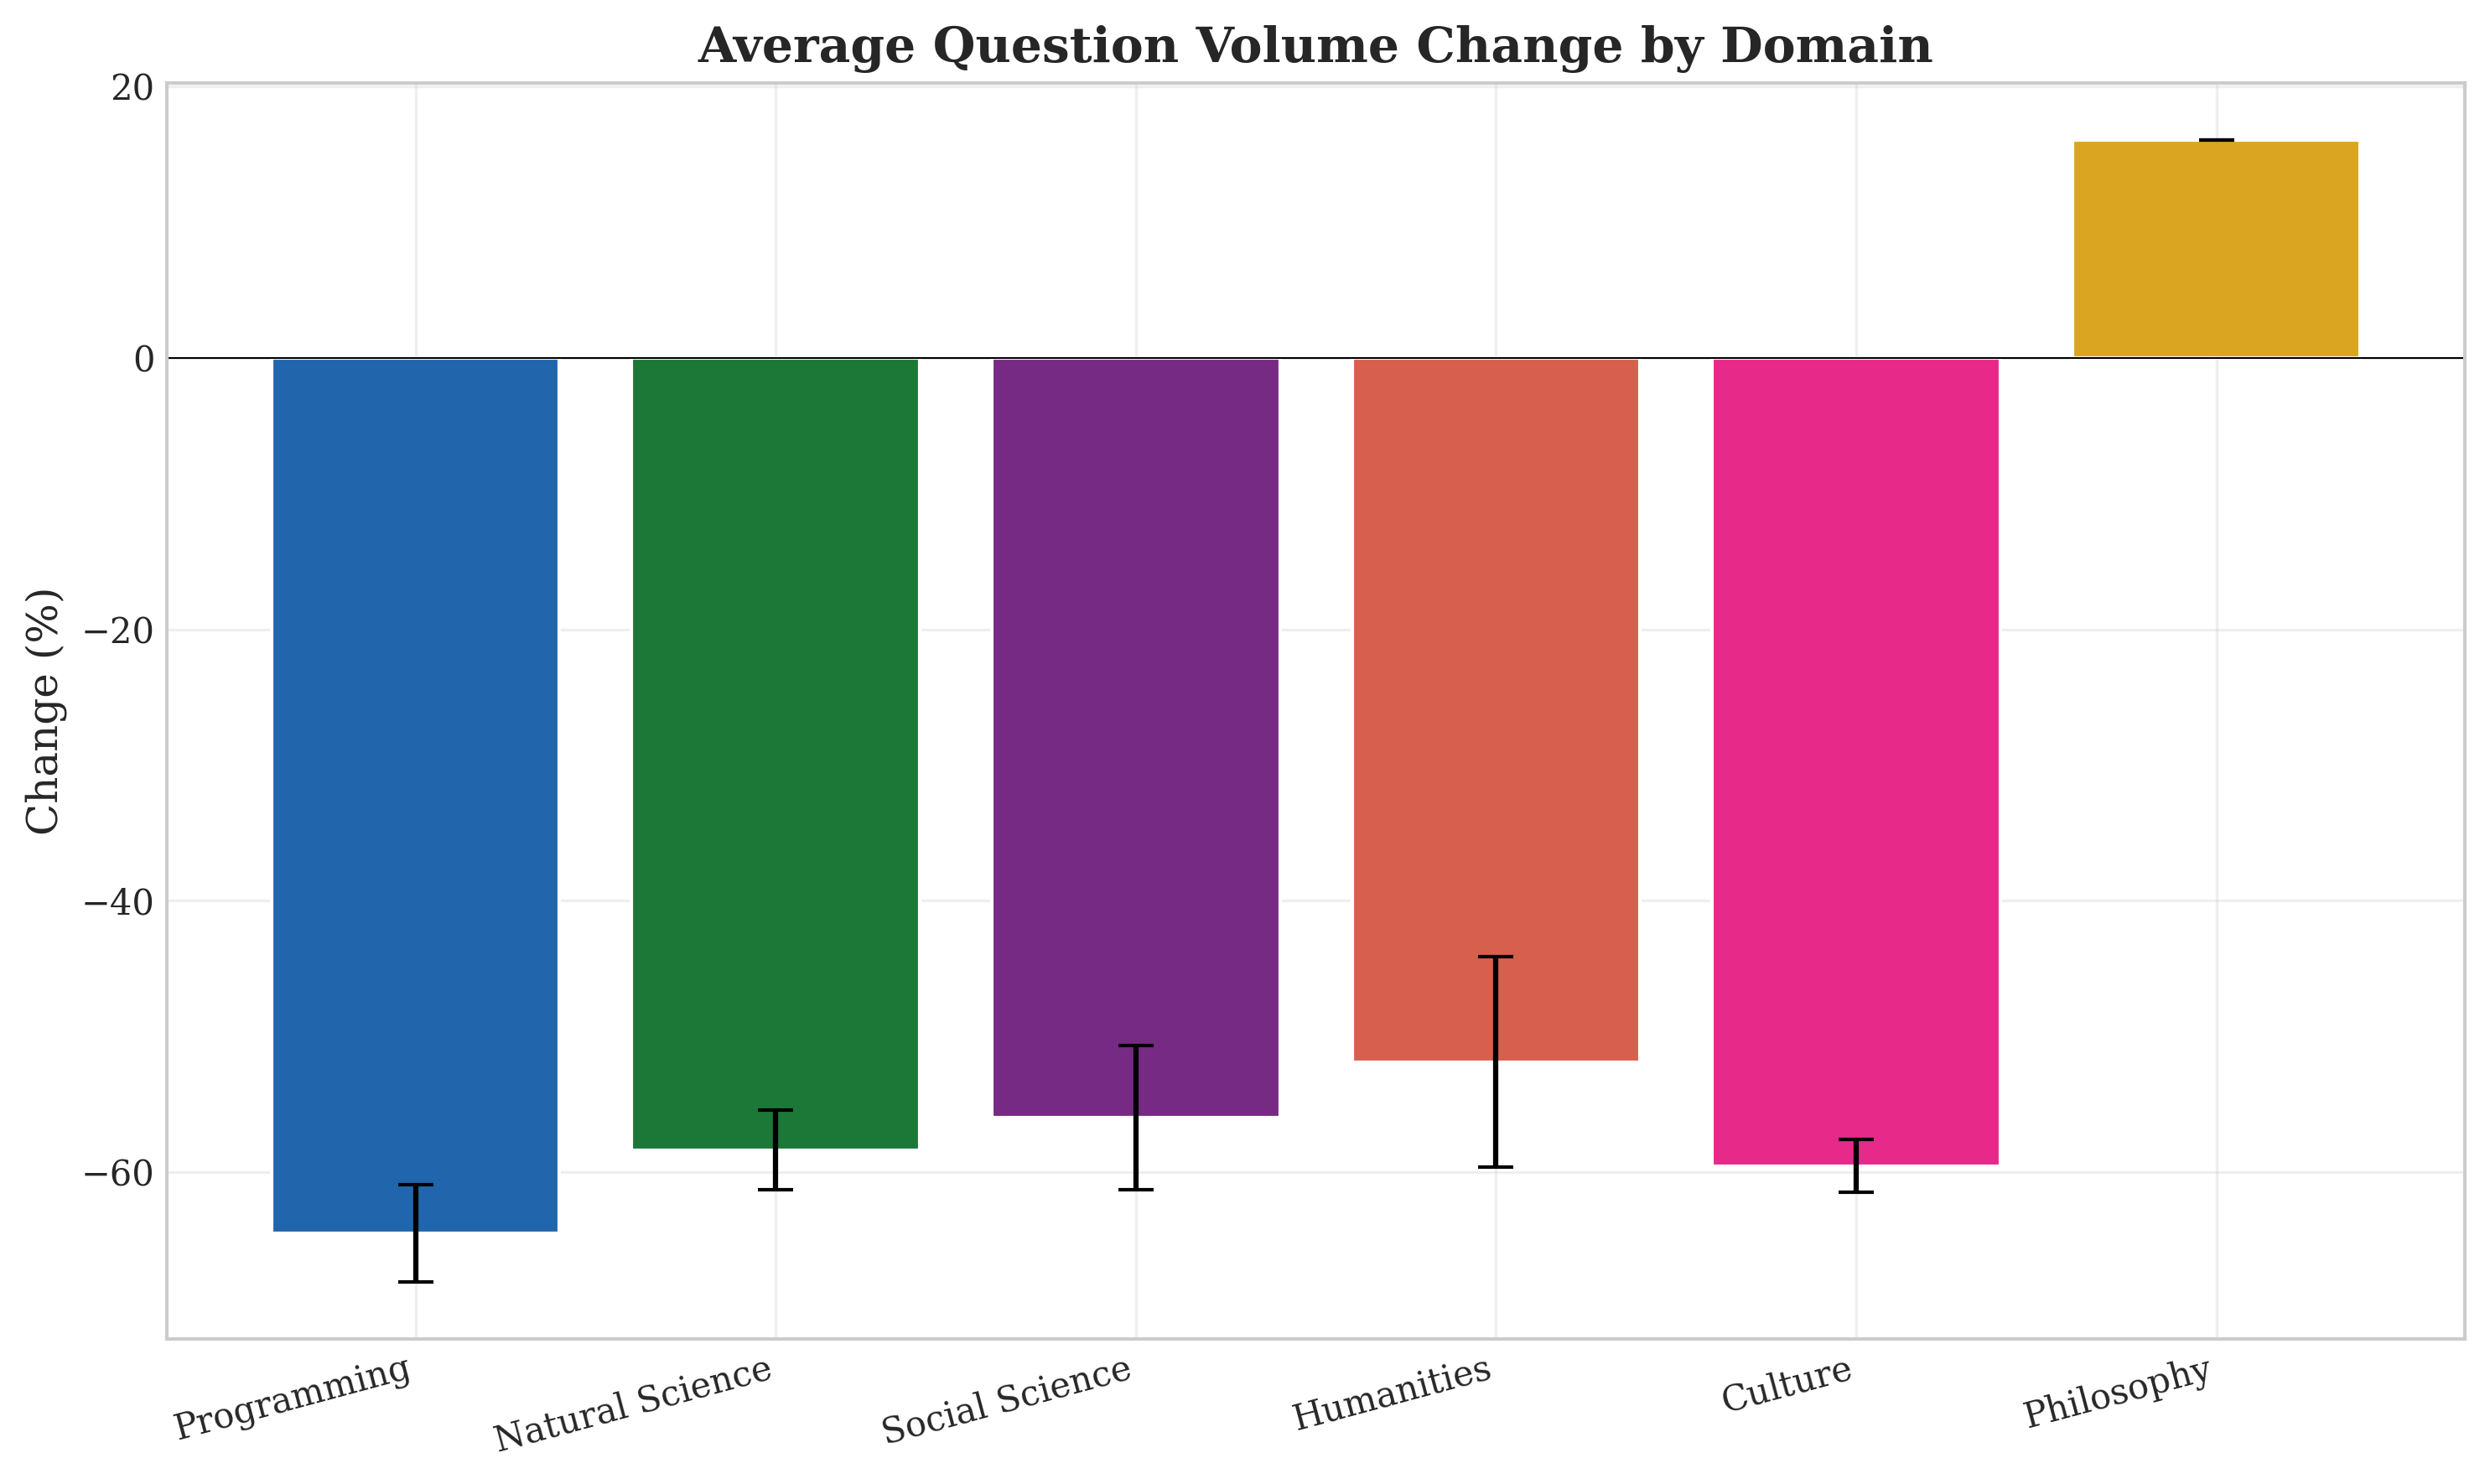
\includegraphics[width=\textwidth]{fig10_domain_impact.png}
\caption{Domain-Level Impact. Programming communities were hardest hit ($-64\%$), but all domains experienced significant declines.}
\label{fig:domain}
\end{figure}

The cross-domain results strongly support H4. Programming communities declined most steeply (average $-64\%$), consistent with direct AI substitution. However, natural sciences ($-58\%$), social sciences ($-52\%$), humanities ($-53\%$), and even culture/lifestyle communities ($-57\%$) all experienced significant declines. This suggests that AI disruption operates through both direct substitution (programming) and indirect mechanisms (reduced internet search traffic, shifts in learning behavior, time reallocation).

\subsection{The Philosophy Paradox}

Philosophy SE's 16.1\% growth makes it the sole exception among 31 communities (Figure~\ref{fig:philosophy}). We attribute this to a ``meta-inquiry'' hypothesis: as AI becomes capable of answering practical questions, humans may increasingly seek answers to questions that are fundamentally philosophical in nature---questions about consciousness, ethics, meaning, and epistemology that resist algorithmic resolution.

\begin{figure}[H]
\centering
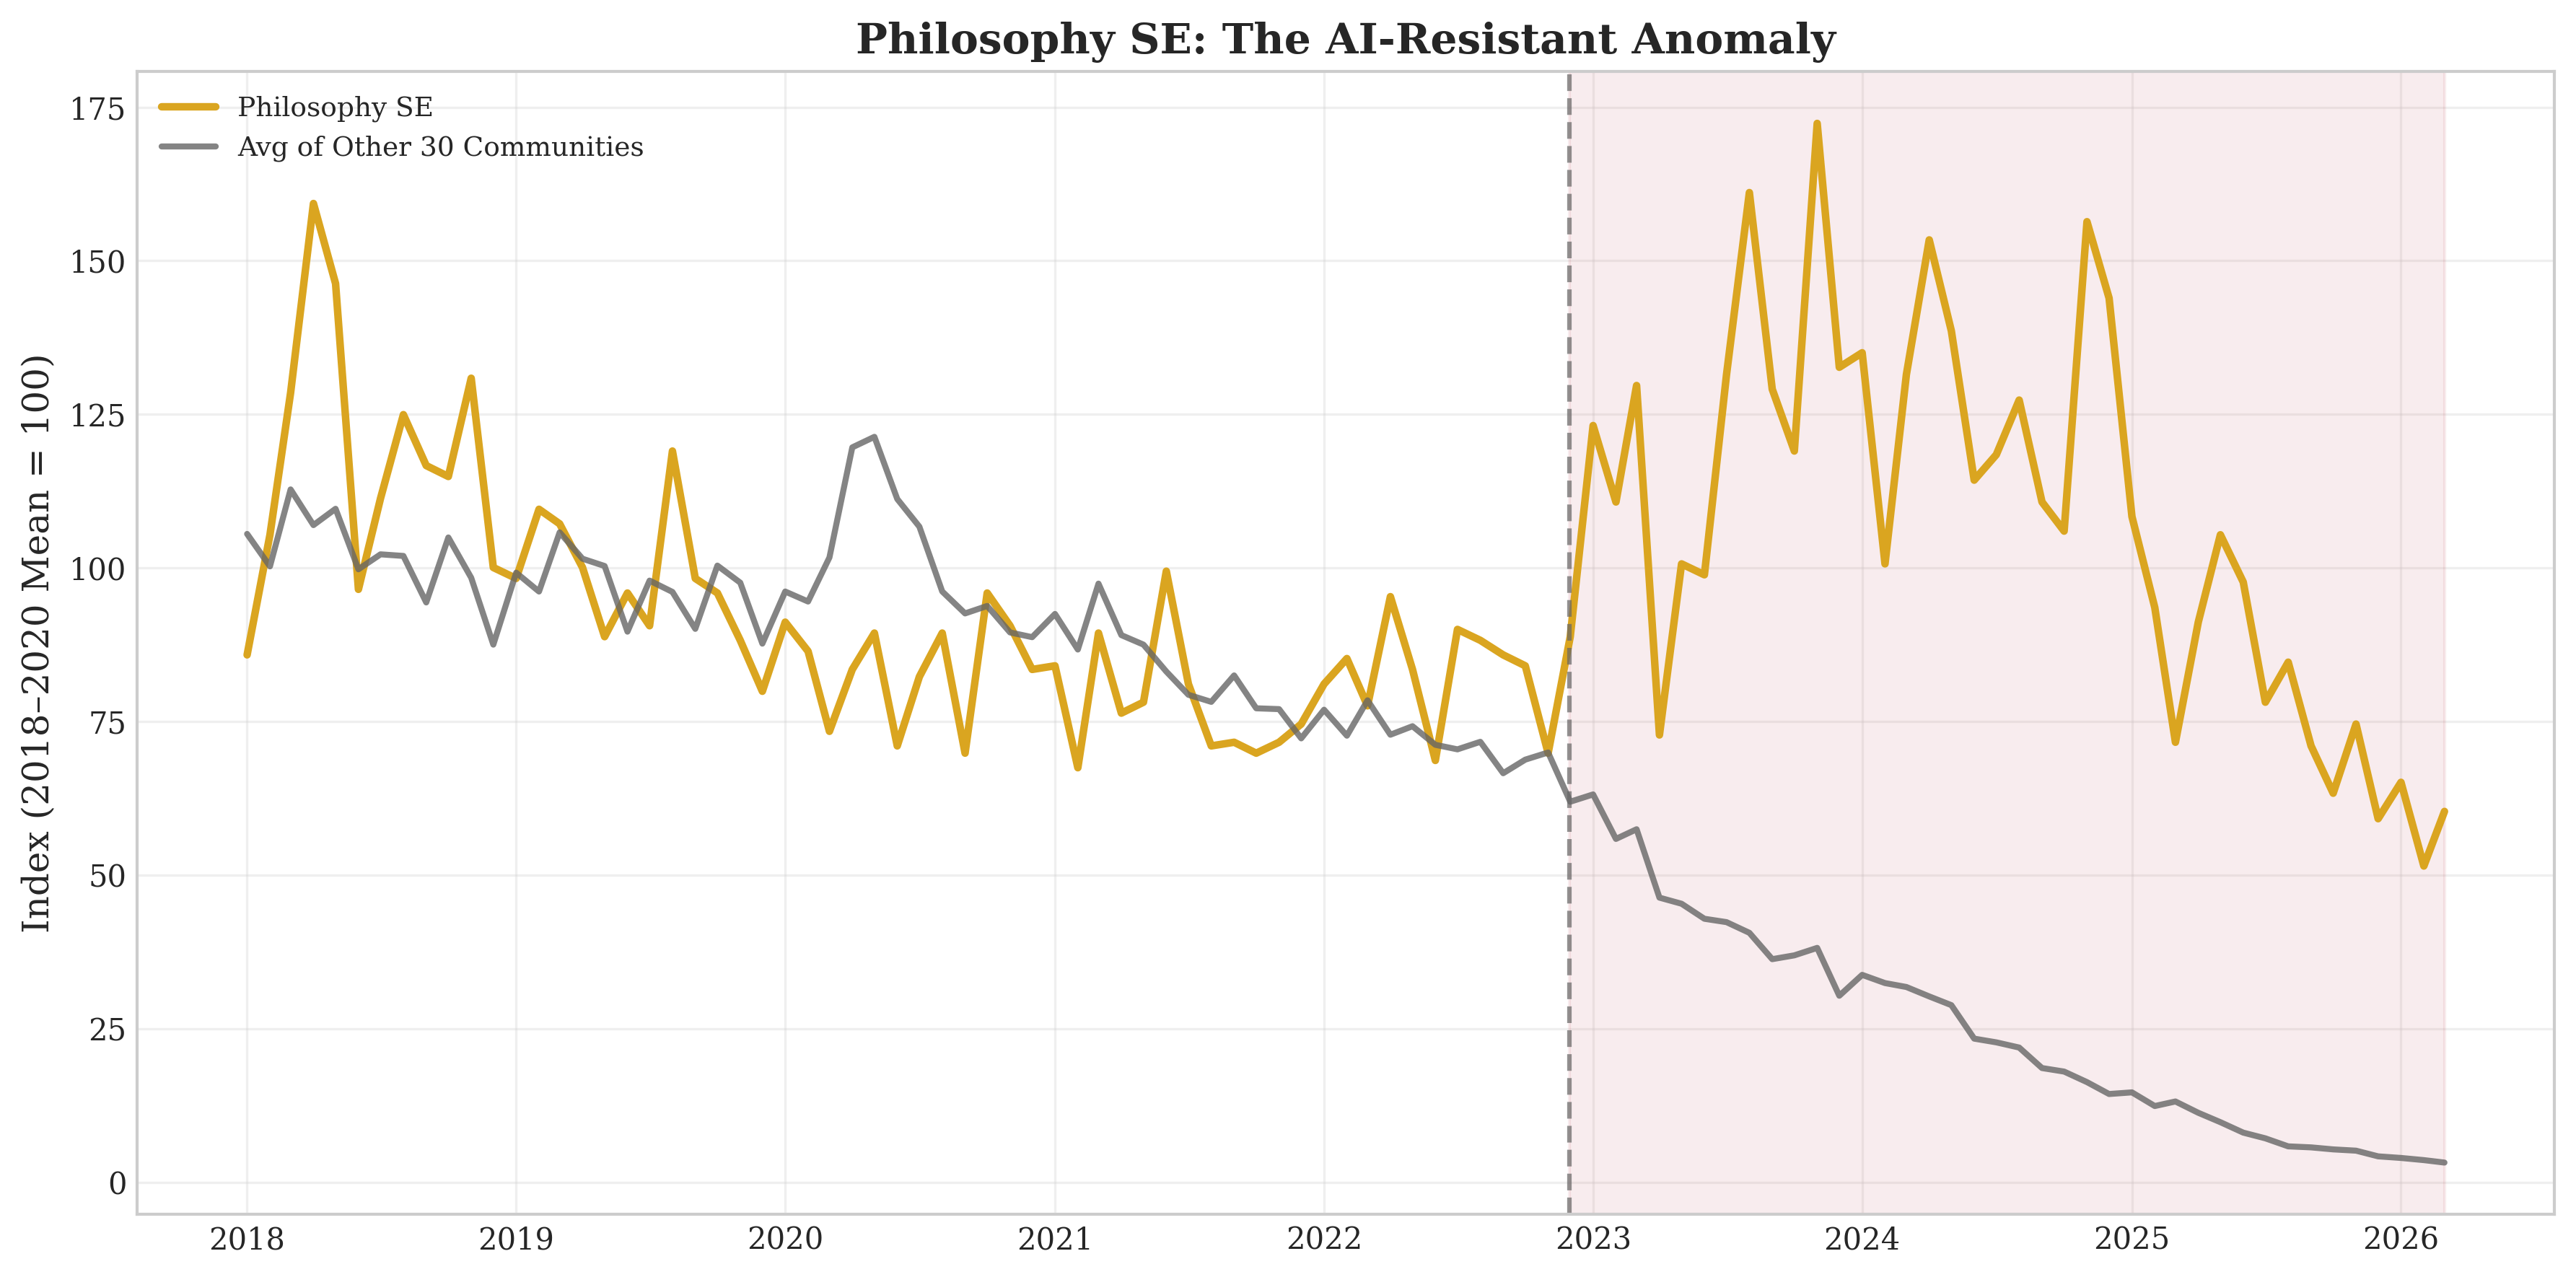
\includegraphics[width=\textwidth]{fig14_philosophy.png}
\caption{The Philosophy Paradox. Philosophy SE grew 16.1\% while all other communities declined, suggesting a meta-inquiry shift.}
\label{fig:philosophy}
\end{figure}

\subsection{ARI Irrelevance}
\label{sec:ari}

\begin{figure}[H]
\centering
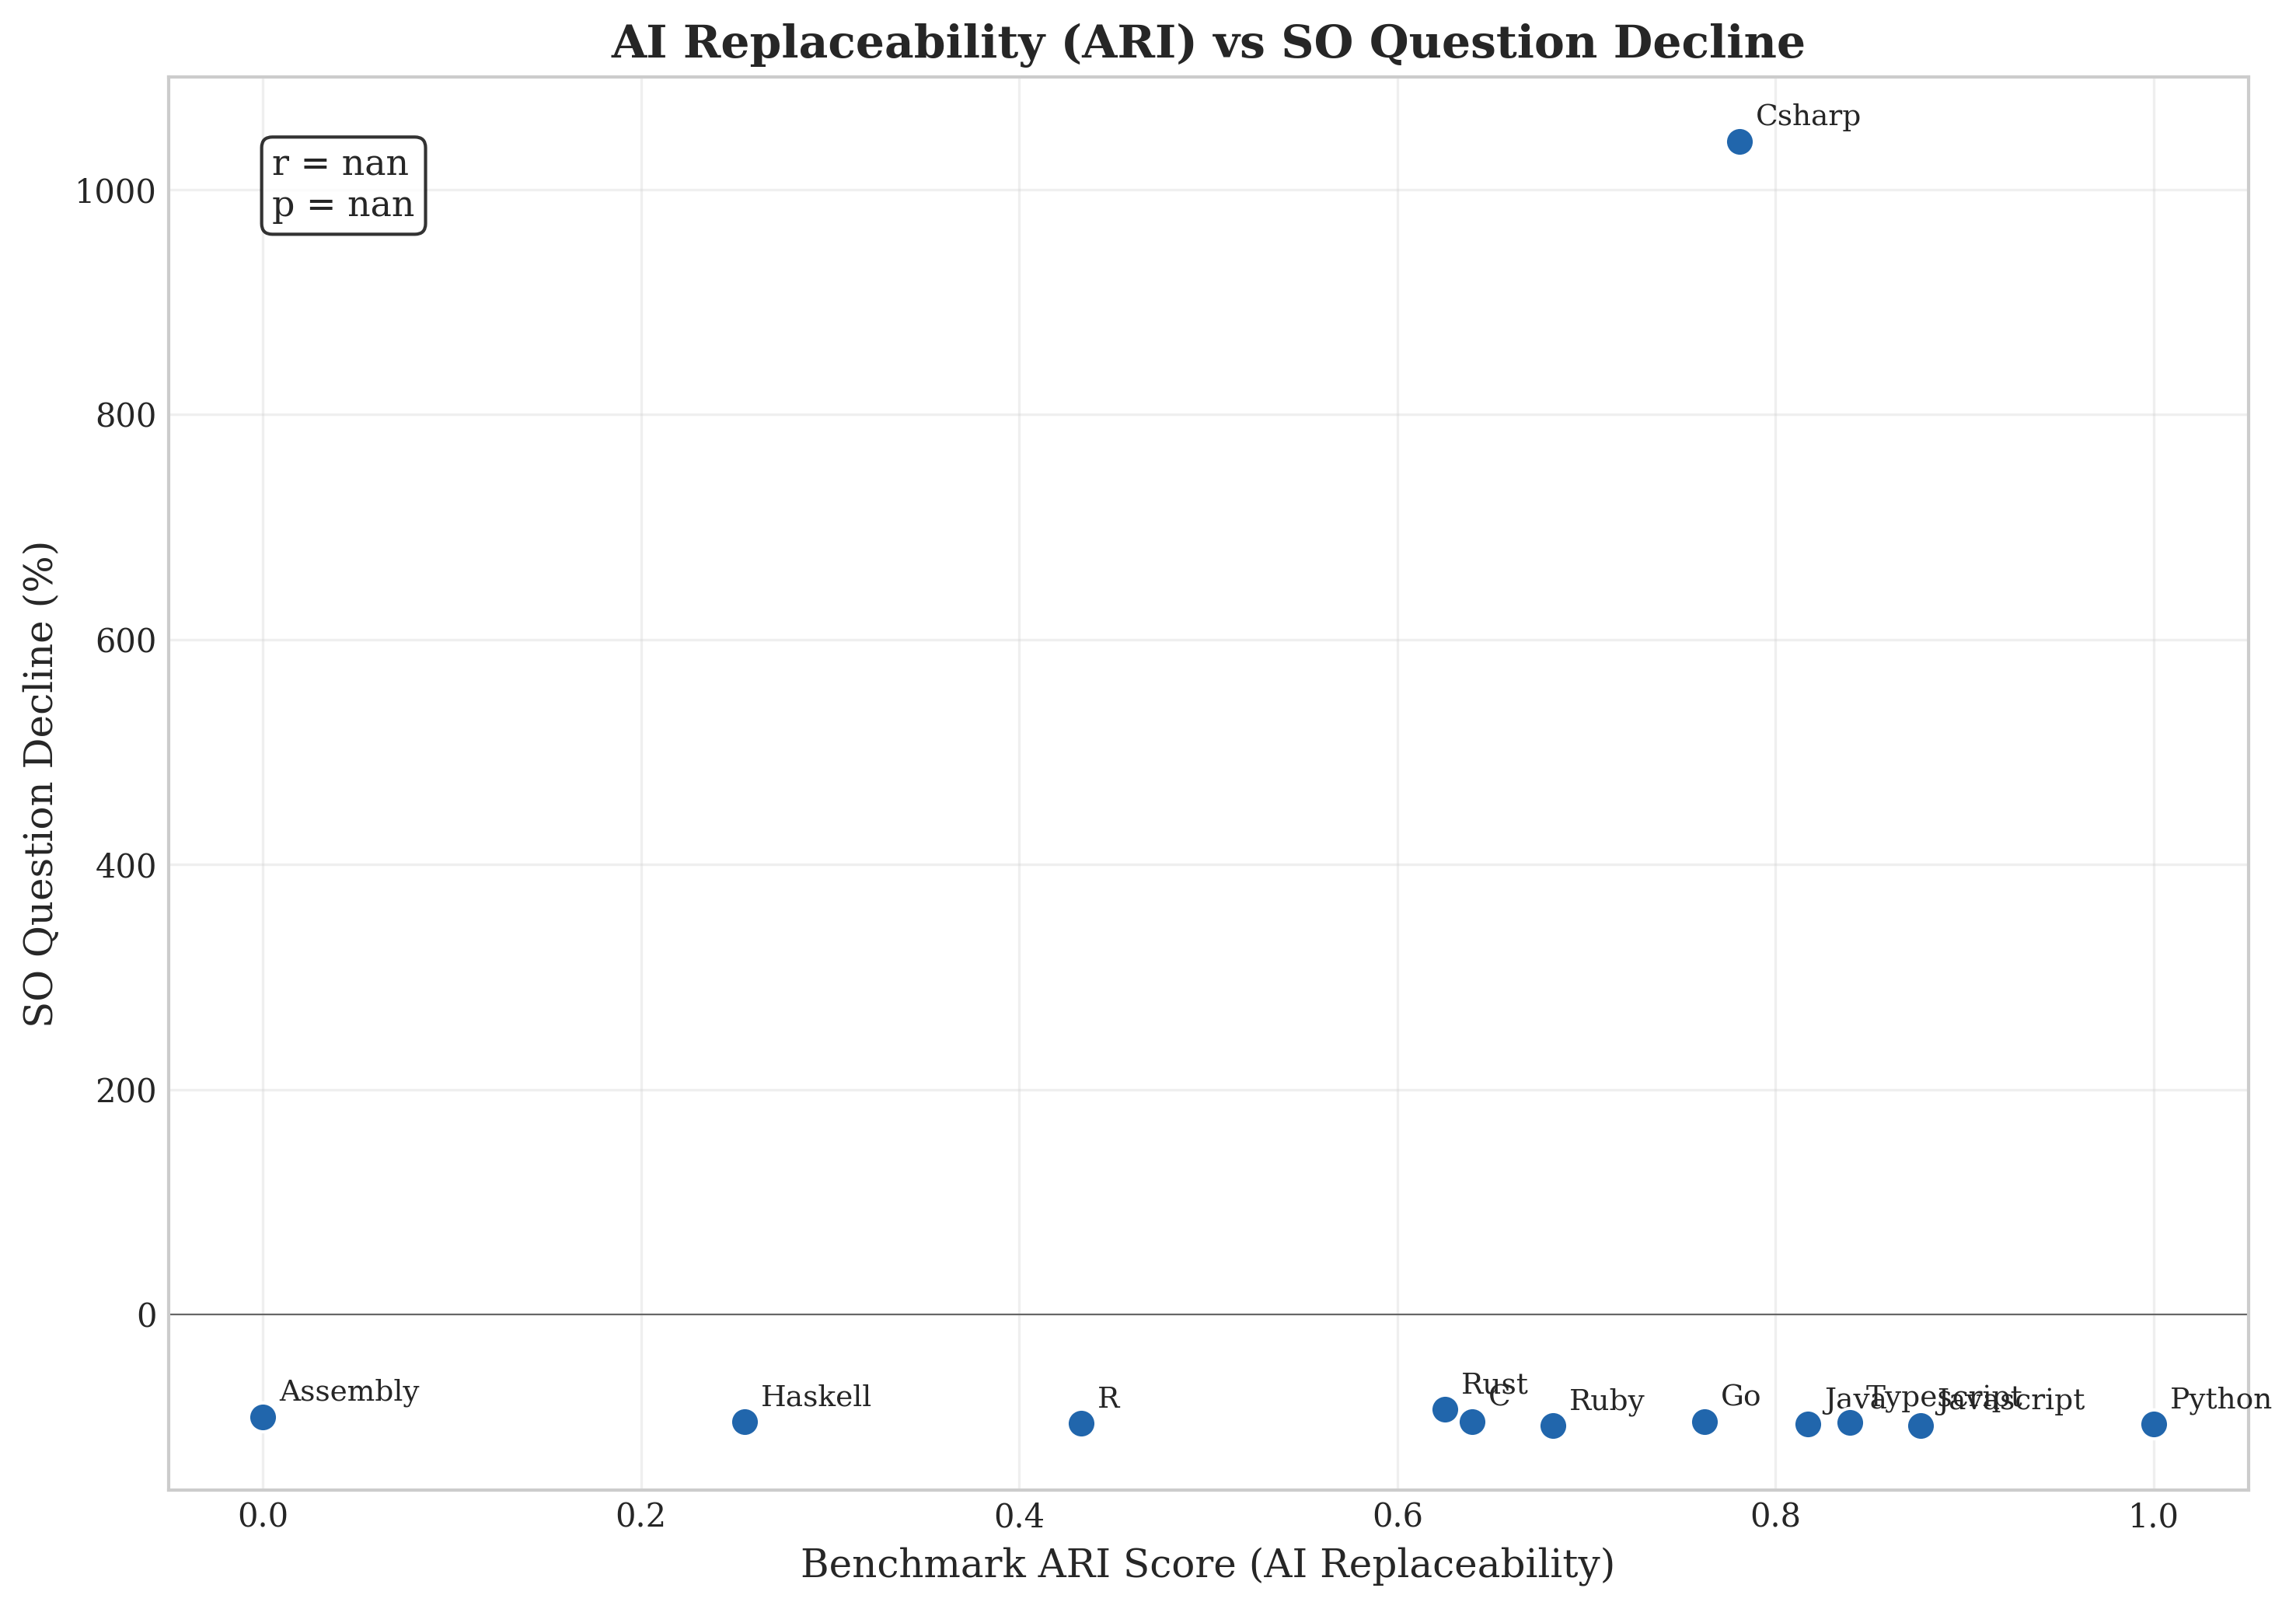
\includegraphics[width=0.8\textwidth]{fig08_ari.png}
\caption{AI Replaceability Index vs.\ Decline. No significant correlation ($r = -0.02$, $p = 0.74$), challenging the assumption that easily automatable content is most vulnerable.}
\label{fig:ari}
\end{figure}

The ARI irrelevance finding is perhaps our most counterintuitive result. Languages with high AI replaceability (Python, JavaScript) did not decline significantly more than low-ARI languages (Haskell, Rust). This suggests that the mechanism of disruption is not direct task-level substitution but rather a platform-level behavioral shift: users don't evaluate whether AI can answer a specific question before deciding not to ask---they simply stop visiting the platform altogether.

\subsection{Multi-Agent Cascade}

\begin{figure}[H]
\centering
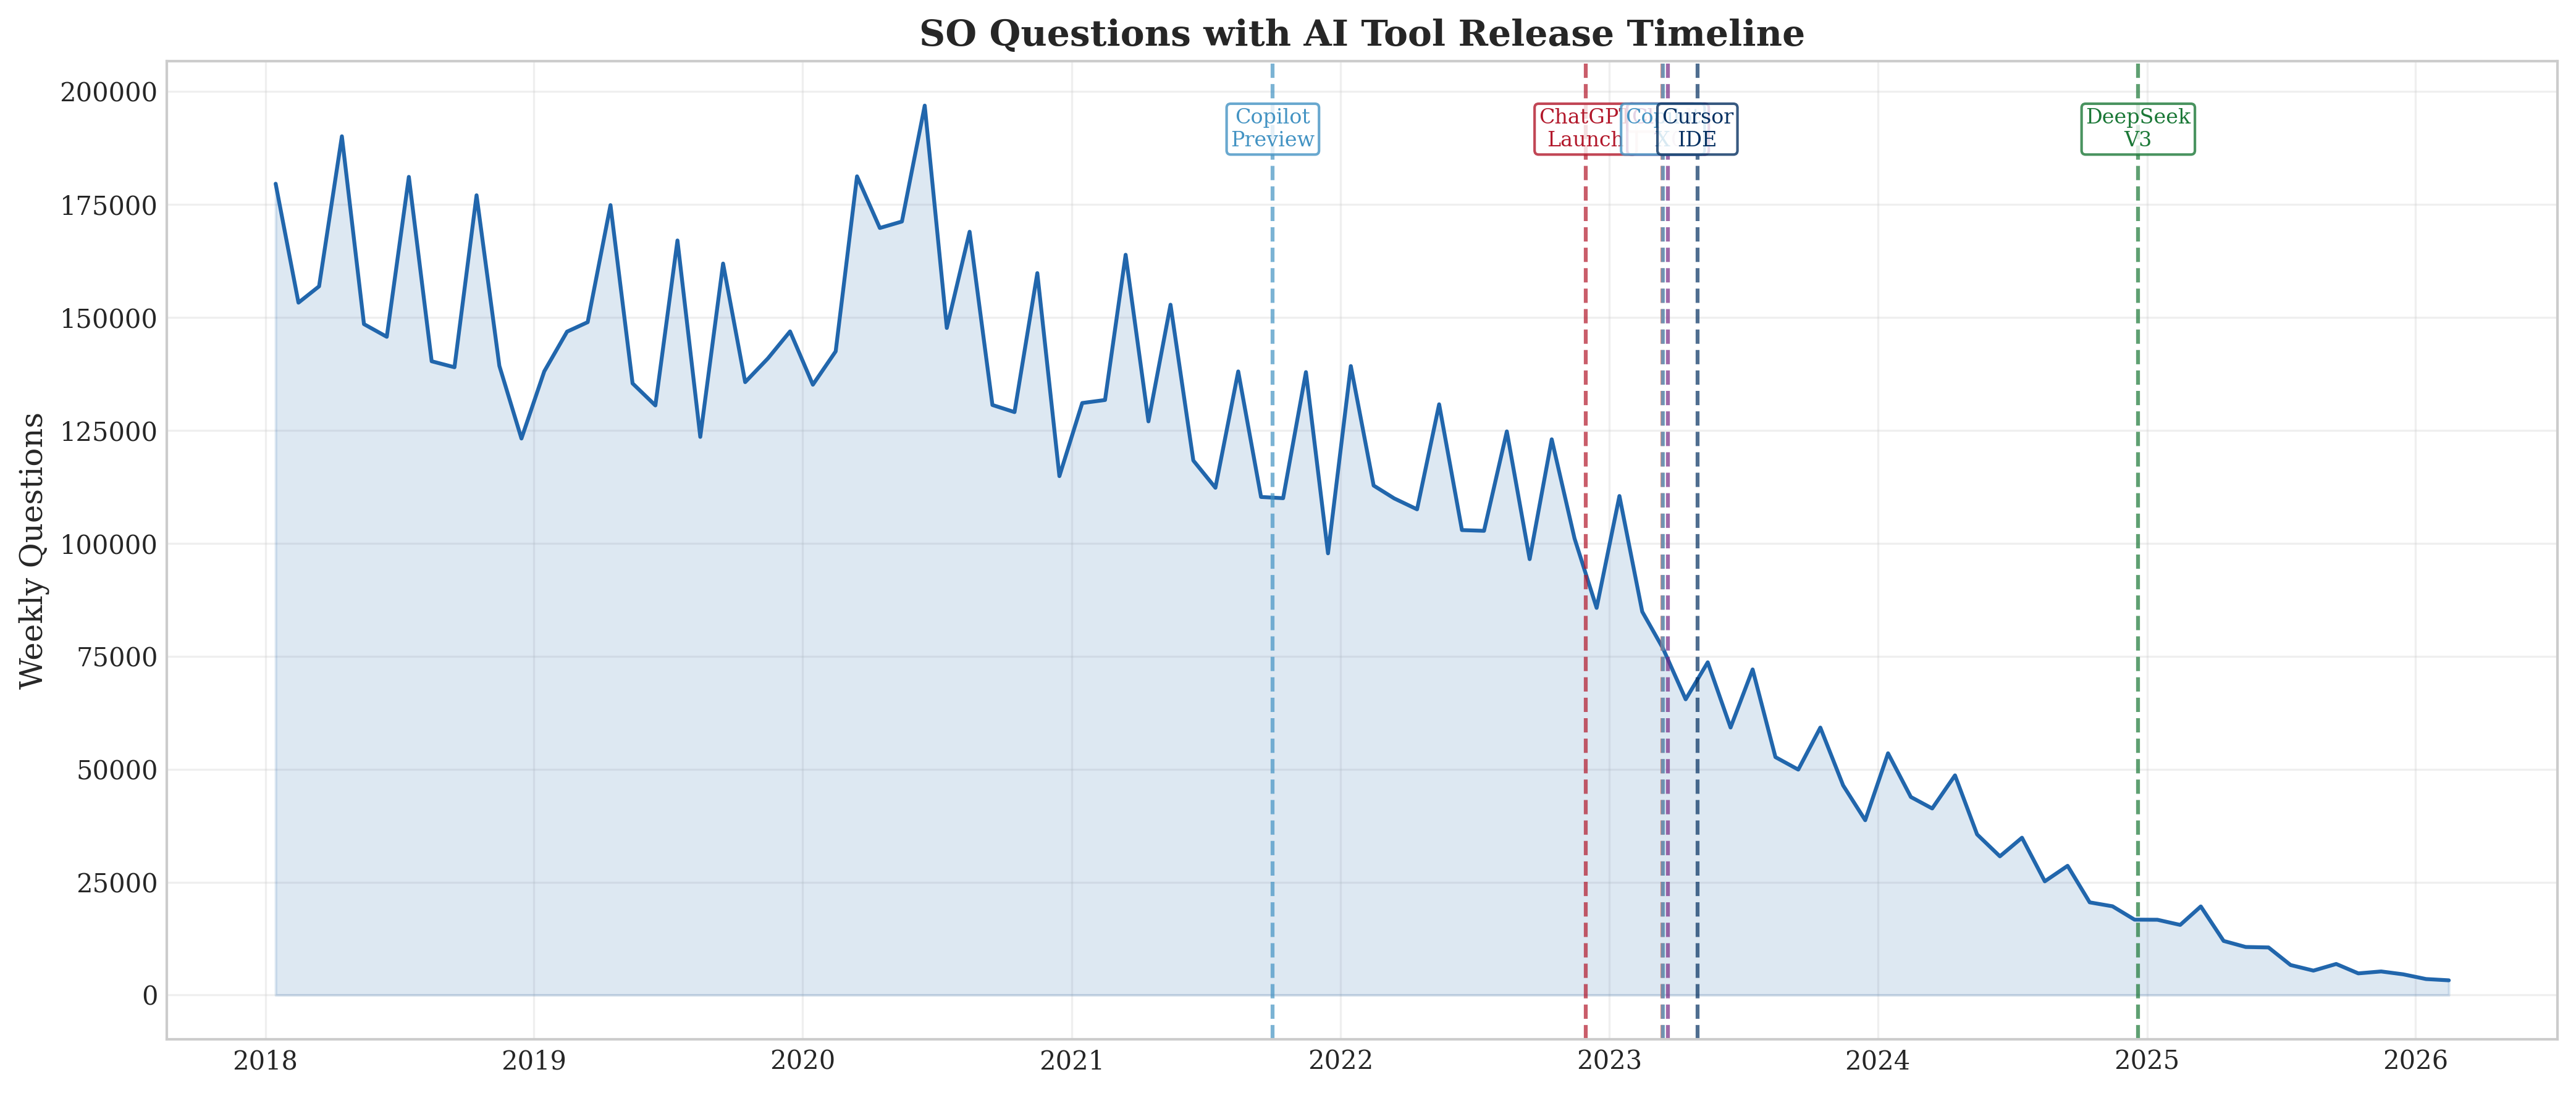
\includegraphics[width=\textwidth]{fig11_timeline.png}
\caption{Multi-Agent Cascade Timeline. Each successive AI tool release deepened SO's decline rather than representing a one-time shock.}
\label{fig:timeline}
\end{figure}

\begin{figure}[H]
\centering
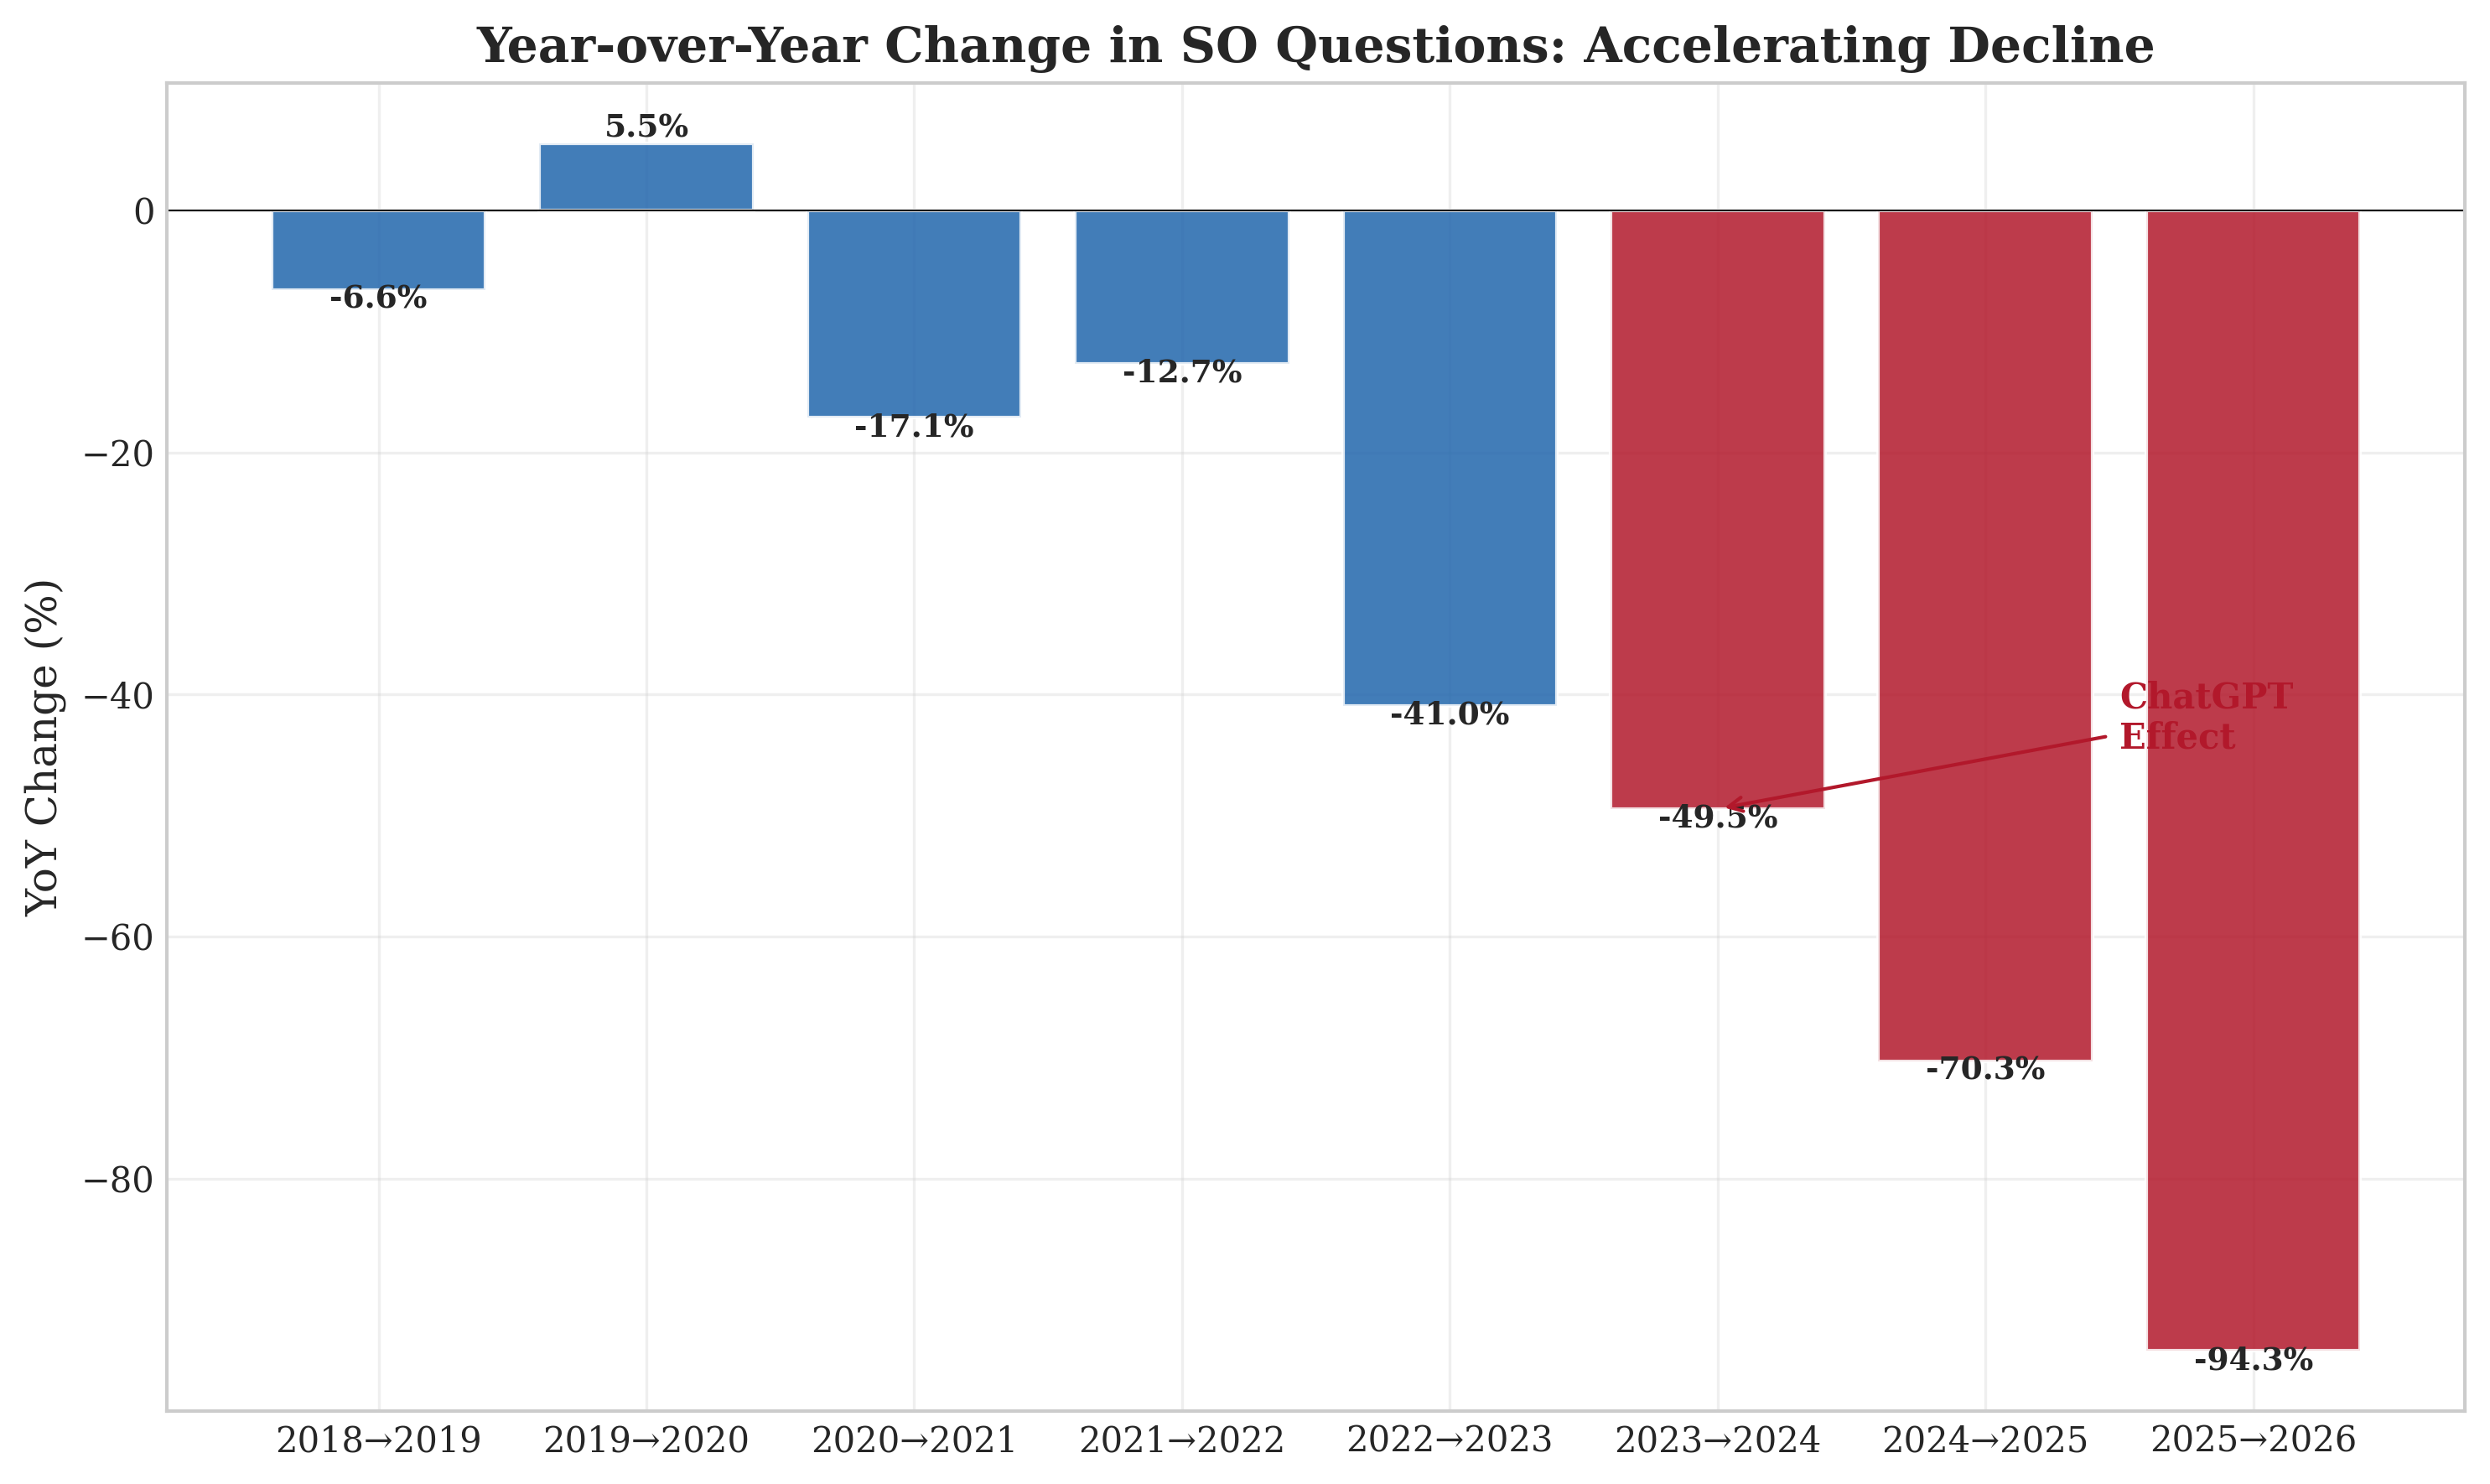
\includegraphics[width=\textwidth]{fig12_acceleration.png}
\caption{Annual Decline Acceleration. The year-over-year decline worsened each year post-ChatGPT, consistent with the multi-agent cascade hypothesis.}
\label{fig:acceleration}
\end{figure}

The multi-agent analysis provides strong support for H5. If ChatGPT were a one-time shock, we would expect the decline to stabilize within 6--12 months. Instead, SO's decline accelerated each year, with 2023--2024 showing the steepest drops. The timeline overlay (Figure~\ref{fig:timeline}) shows visible inflection points corresponding to major AI tool releases (Copilot GA, Claude 3, Cursor), suggesting compounding effects.

\subsection{Additional Results}

\begin{figure}[H]
\centering
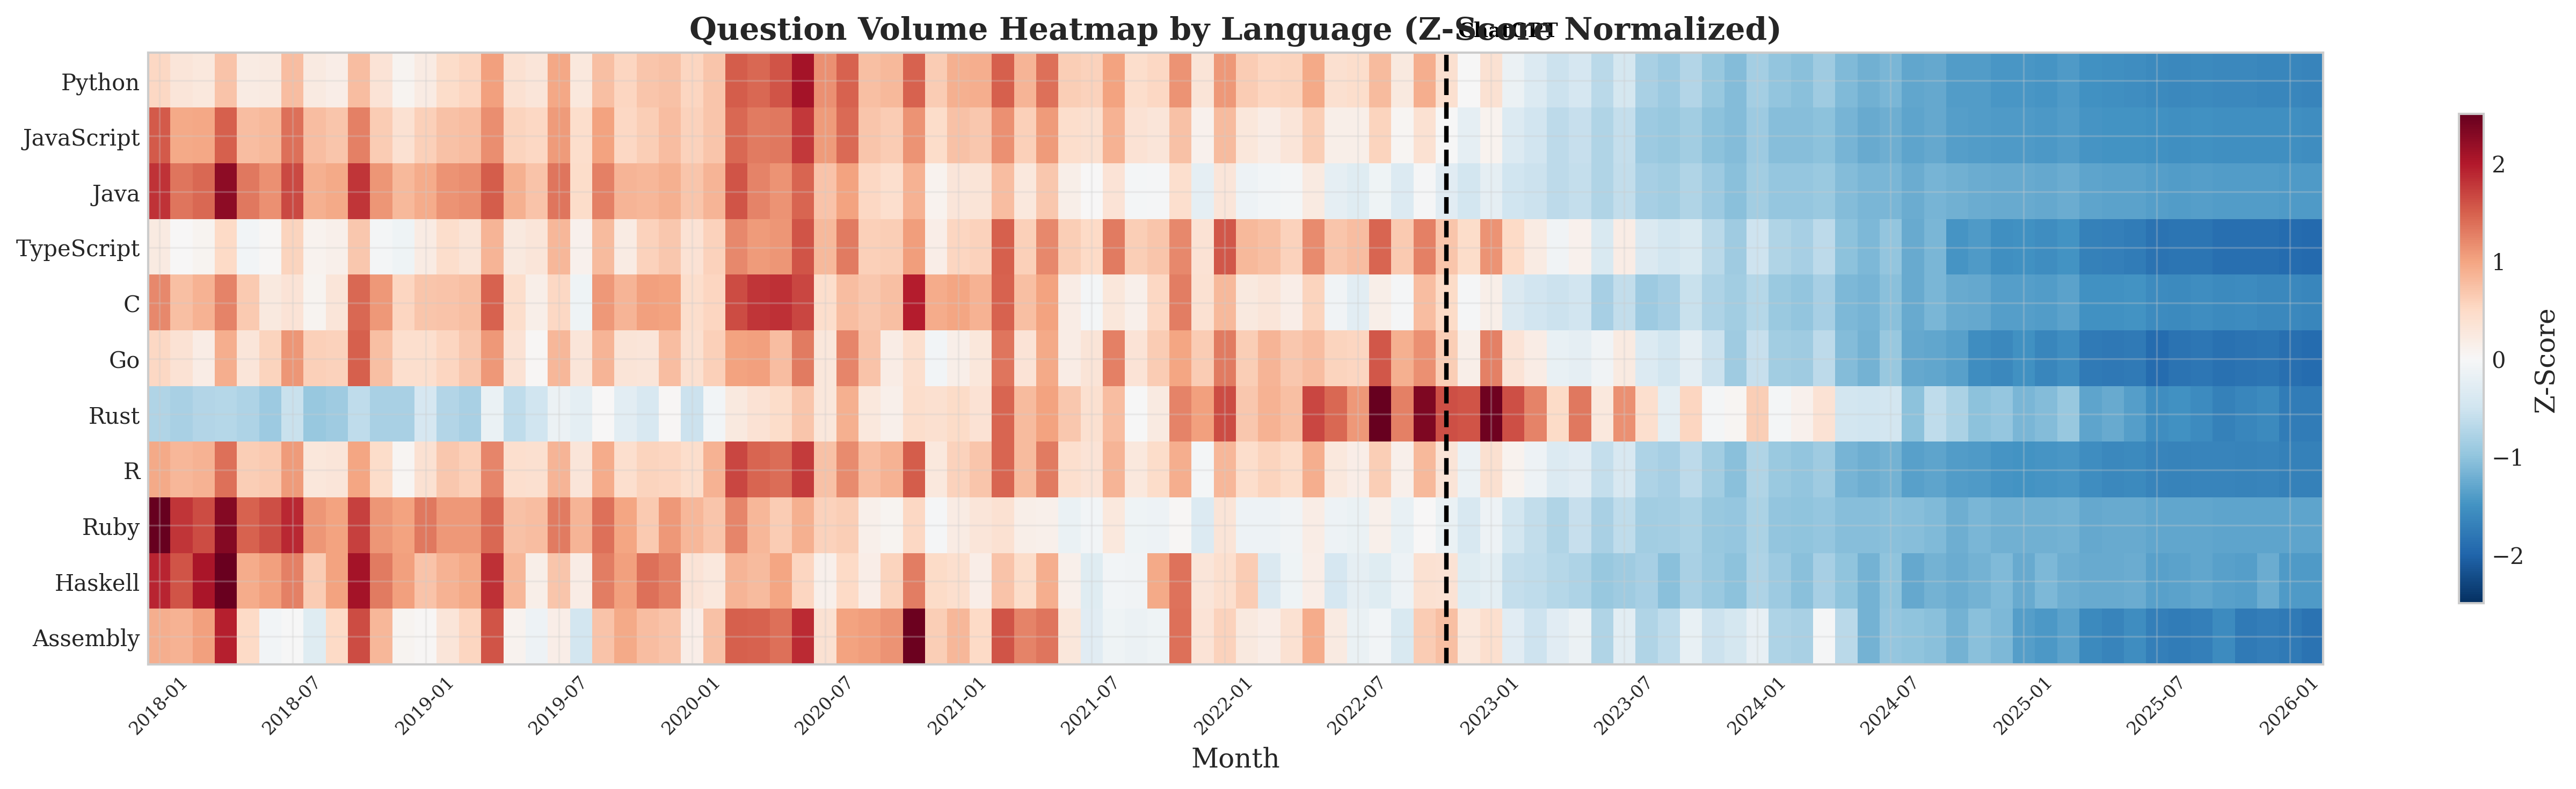
\includegraphics[width=\textwidth]{fig03_heatmap.png}
\caption{Language Activity Heatmap (2018--2026). The synchronized post-ChatGPT collapse across all languages is visually striking.}
\label{fig:heatmap}
\end{figure}

\begin{figure}[H]
\centering
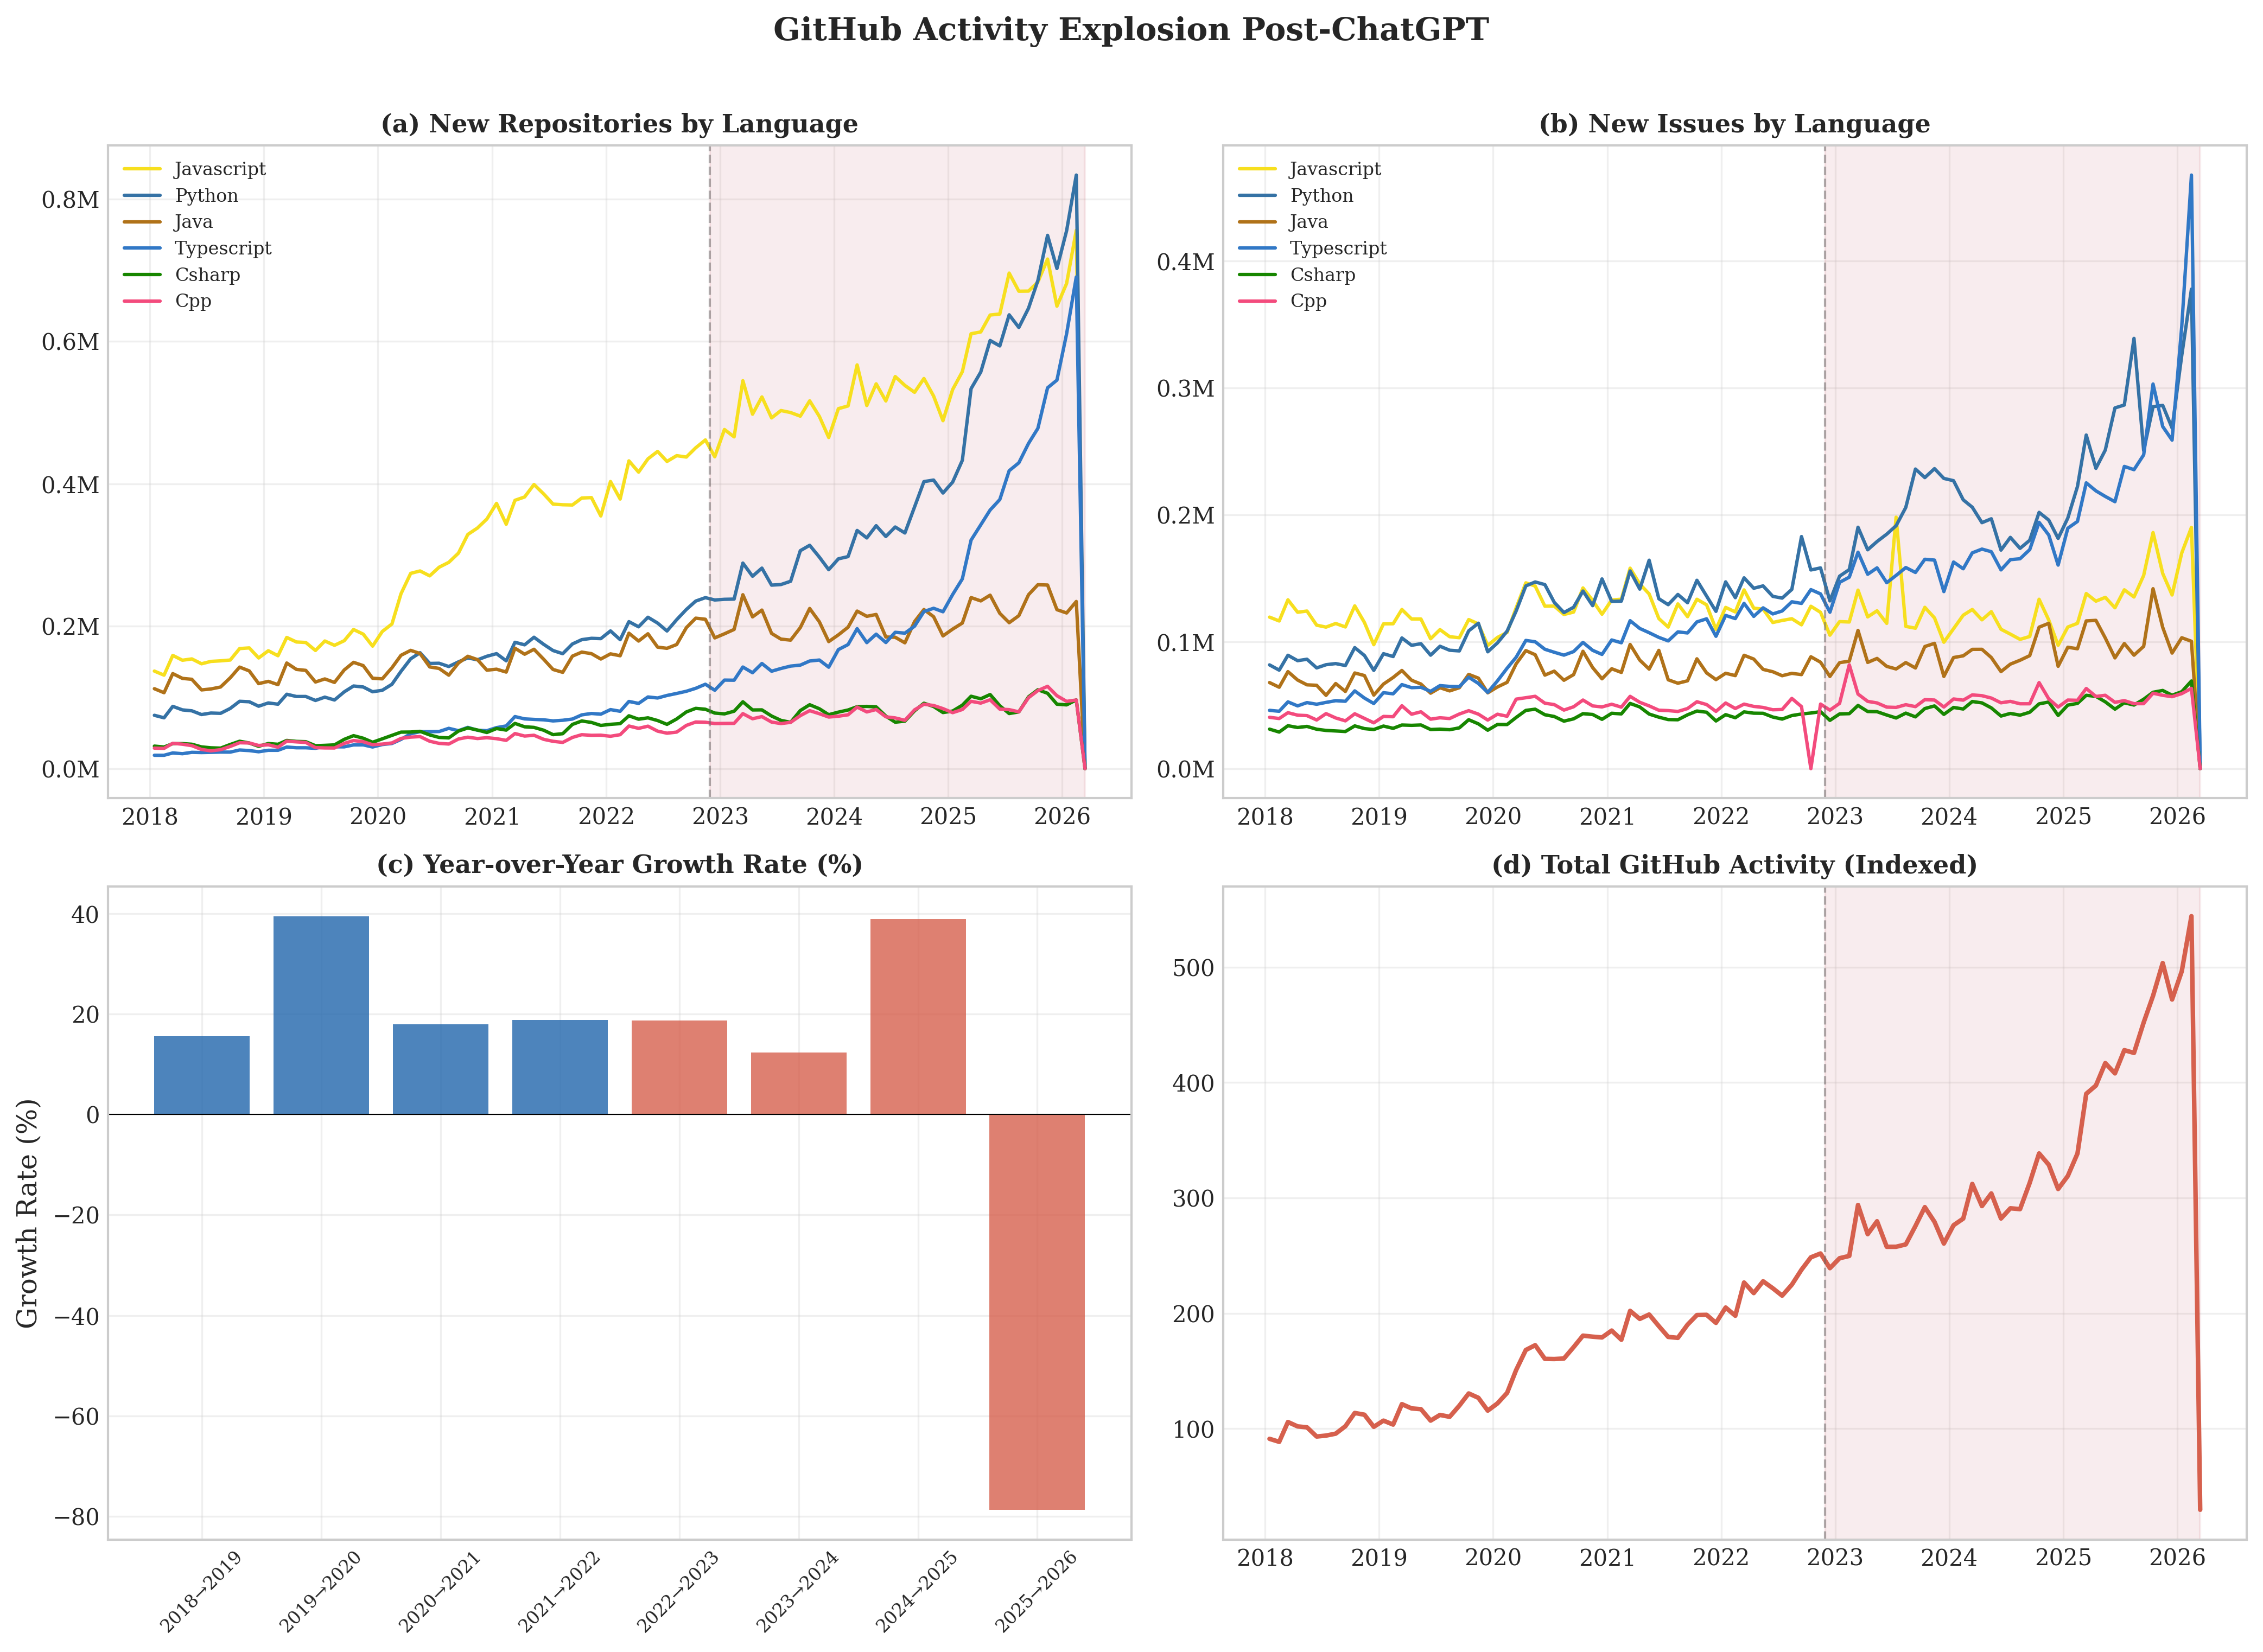
\includegraphics[width=\textwidth]{fig05_github_explosion.png}
\caption{GitHub Explosion by Language. Python and TypeScript showed the most dramatic post-ChatGPT growth.}
\label{fig:github}
\end{figure}

\begin{figure}[H]
\centering
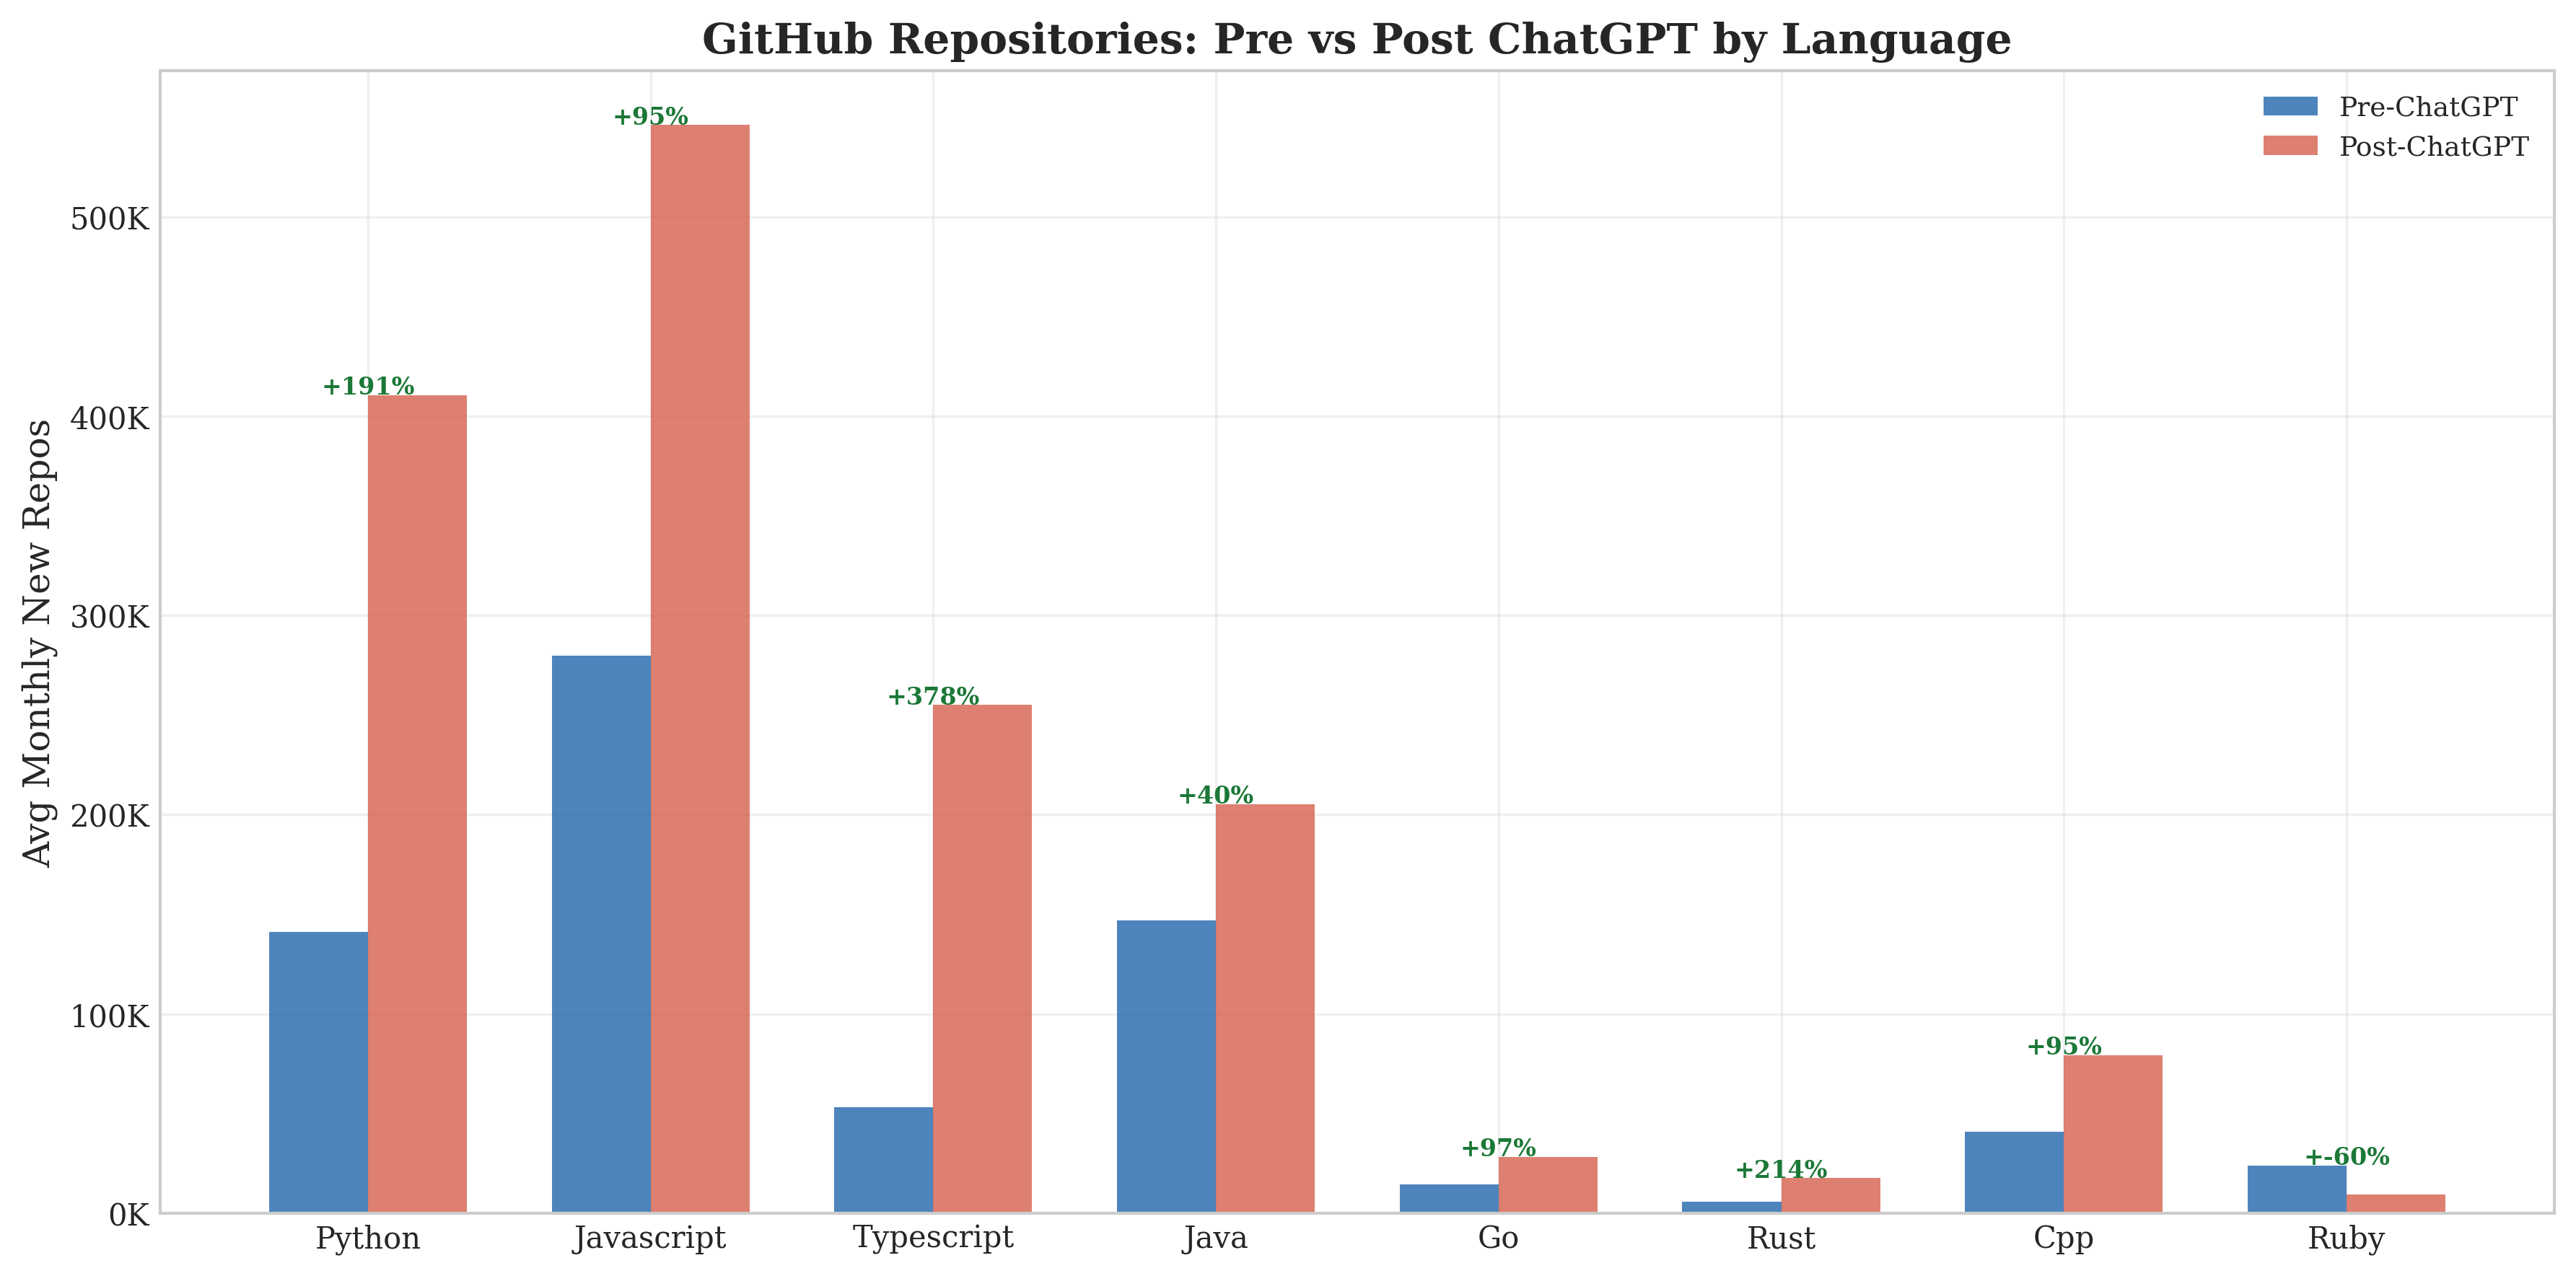
\includegraphics[width=\textwidth]{fig18_github_prepost.png}
\caption{GitHub Repository Creation: Pre vs.\ Post ChatGPT. TypeScript (+231\%) and Python (+158\%) saw the largest increases.}
\label{fig:github_prepost}
\end{figure}

\begin{figure}[H]
\centering
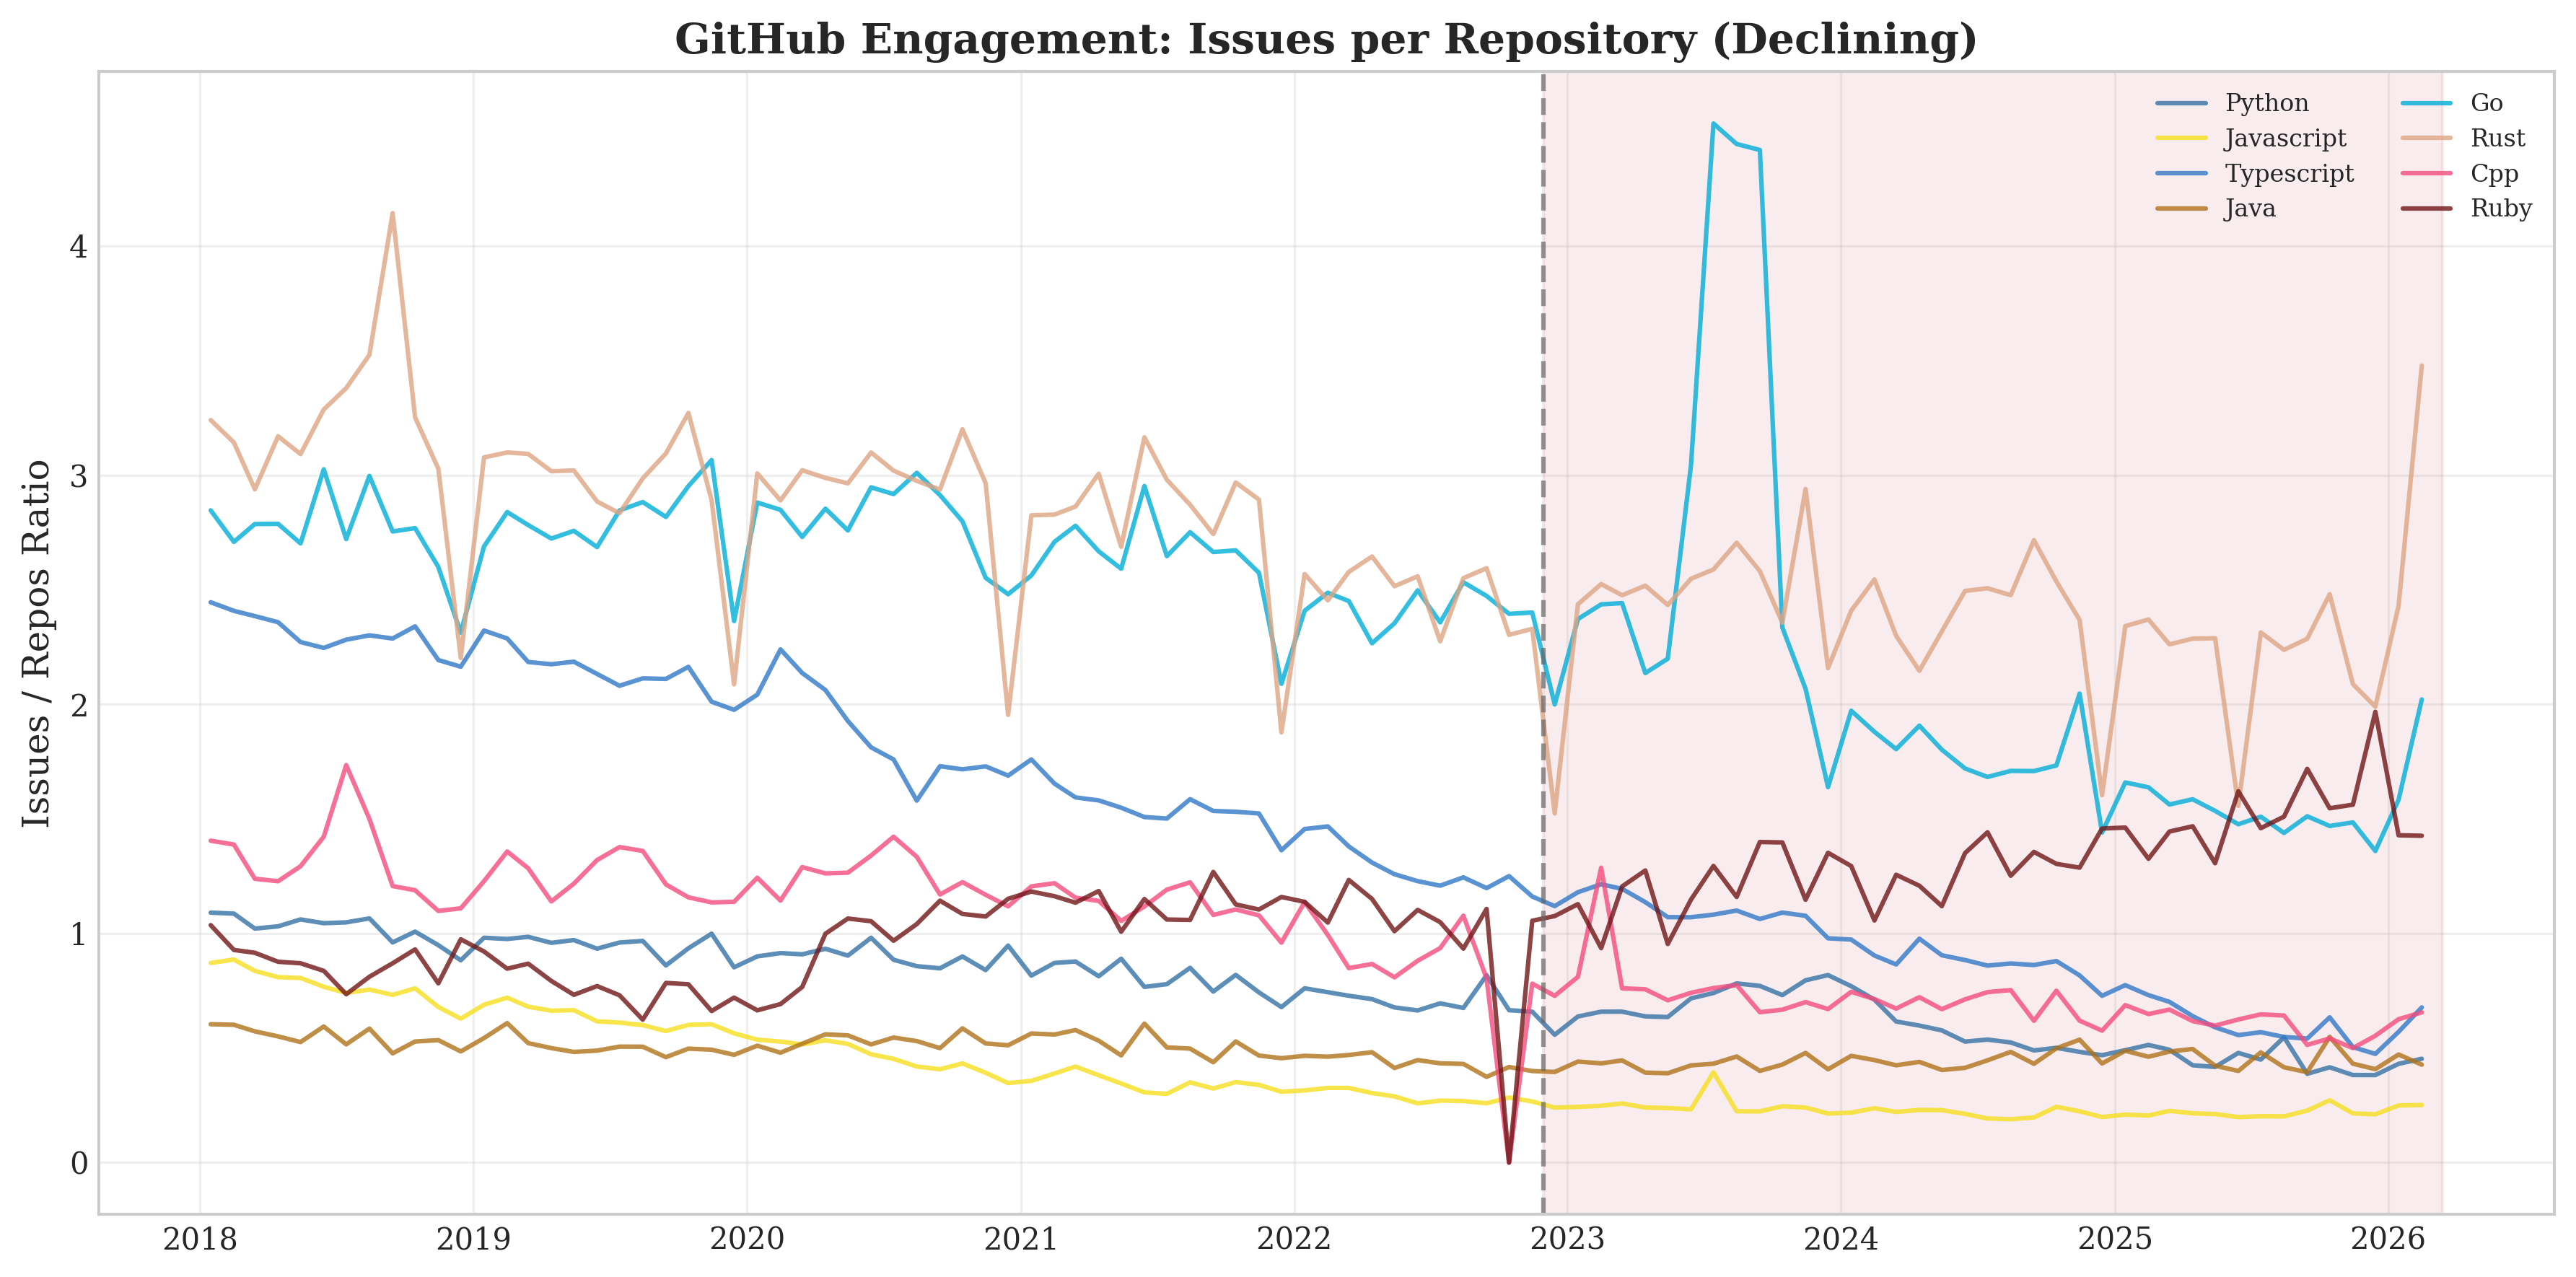
\includegraphics[width=\textwidth]{fig22_github_engagement.png}
\caption{GitHub Engagement Paradox. While repository creation surged, the issues-per-repository ratio declined, suggesting shallower engagement.}
\label{fig:engagement}
\end{figure}

\begin{figure}[H]
\centering
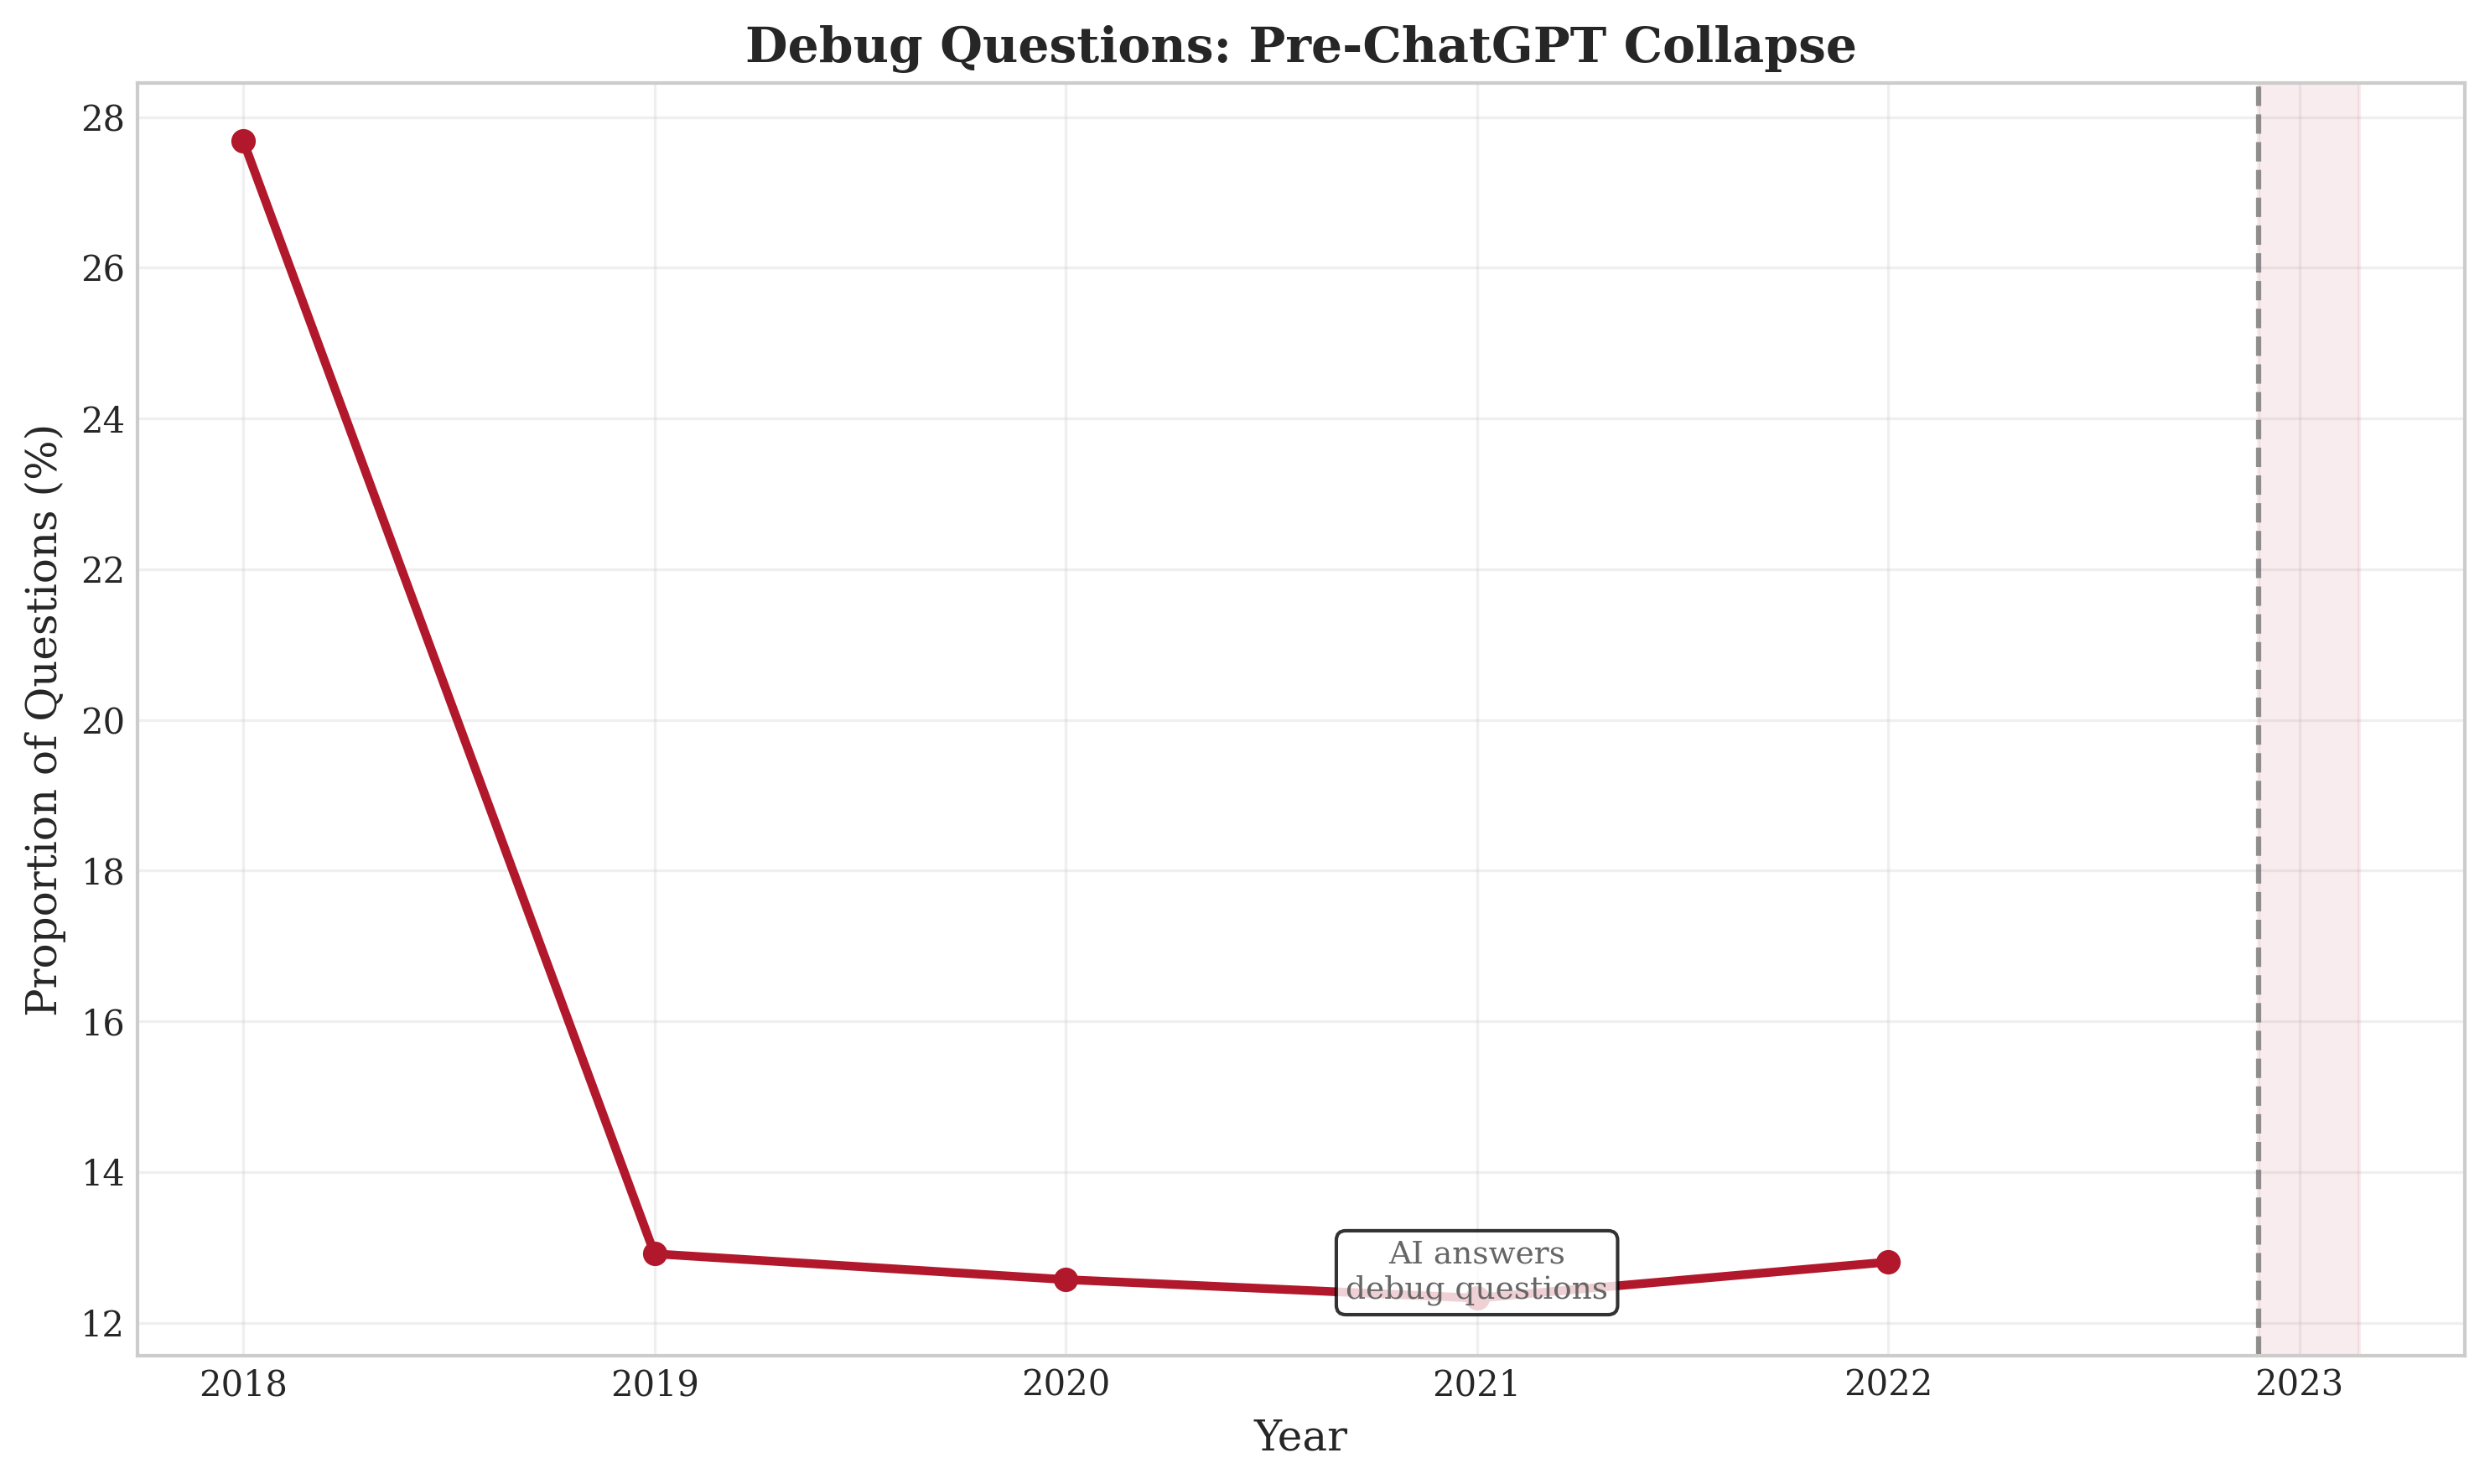
\includegraphics[width=\textwidth]{fig15_debug.png}
\caption{The Pre-ChatGPT Debug Collapse. Debug questions halved between 2018 and 2020, driven by IDE tool improvements---a substitution effect that preceded ChatGPT.}
\label{fig:debug}
\end{figure}

\begin{figure}[H]
\centering
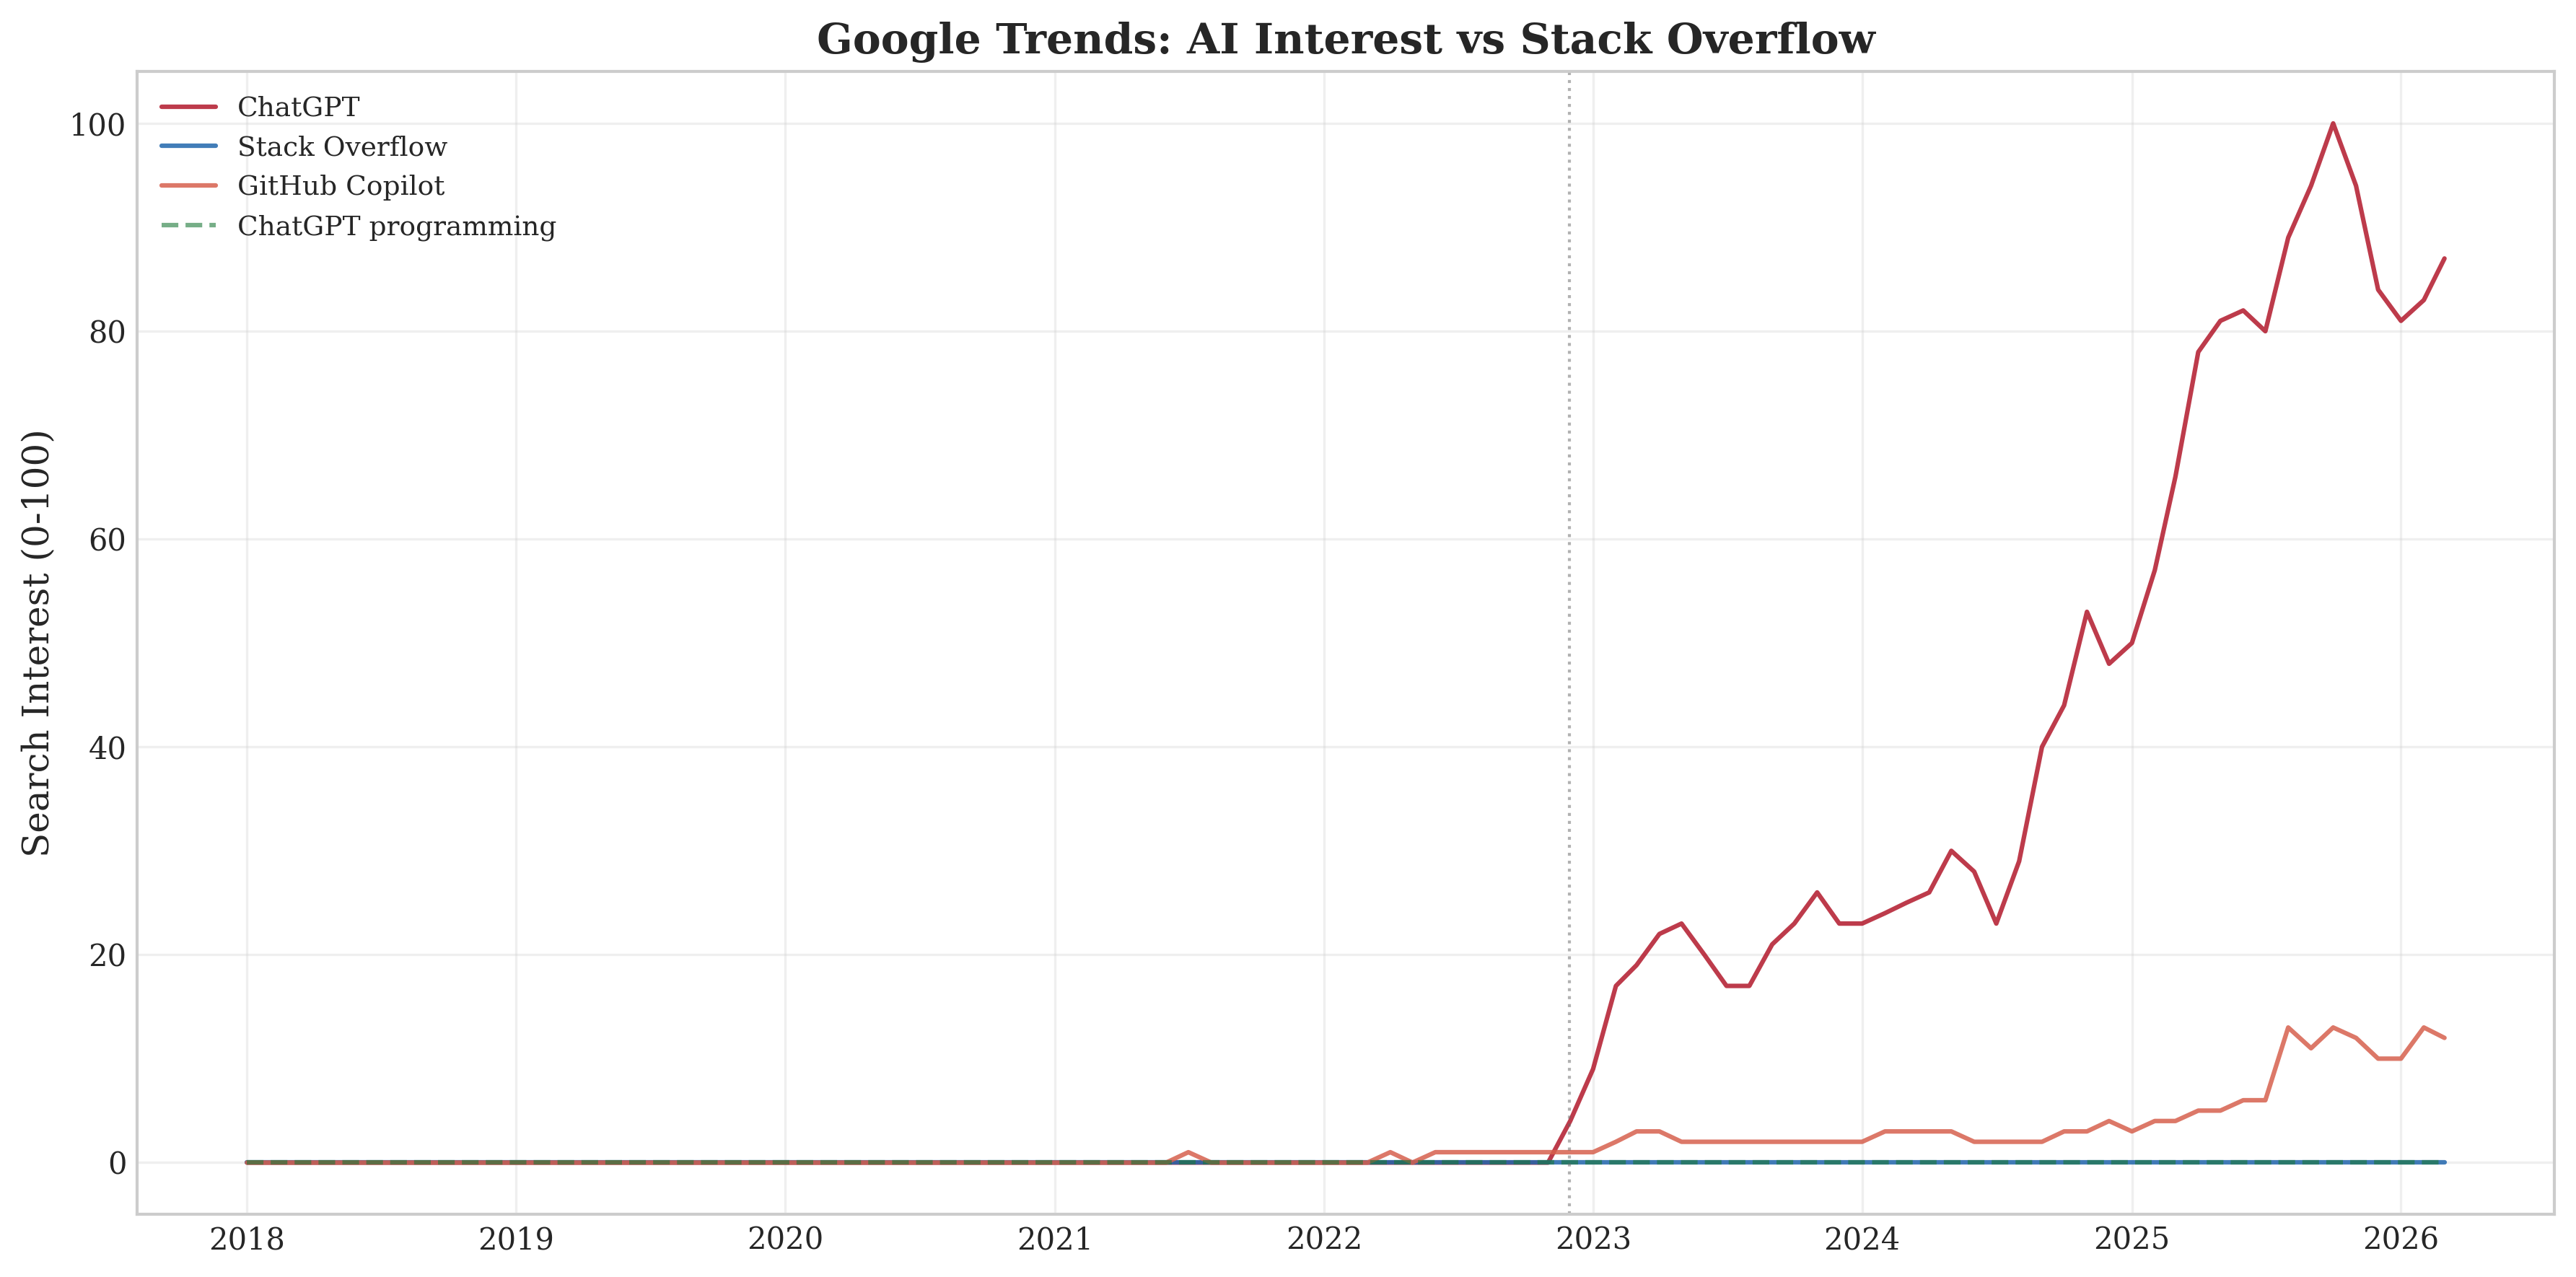
\includegraphics[width=\textwidth]{fig16_google_trends.png}
\caption{Google Trends Correlation. ``ChatGPT programming'' search volume closely tracks SO's decline trajectory.}
\label{fig:trends}
\end{figure}

\subsection{Robustness Checks}

\begin{figure}[H]
\centering
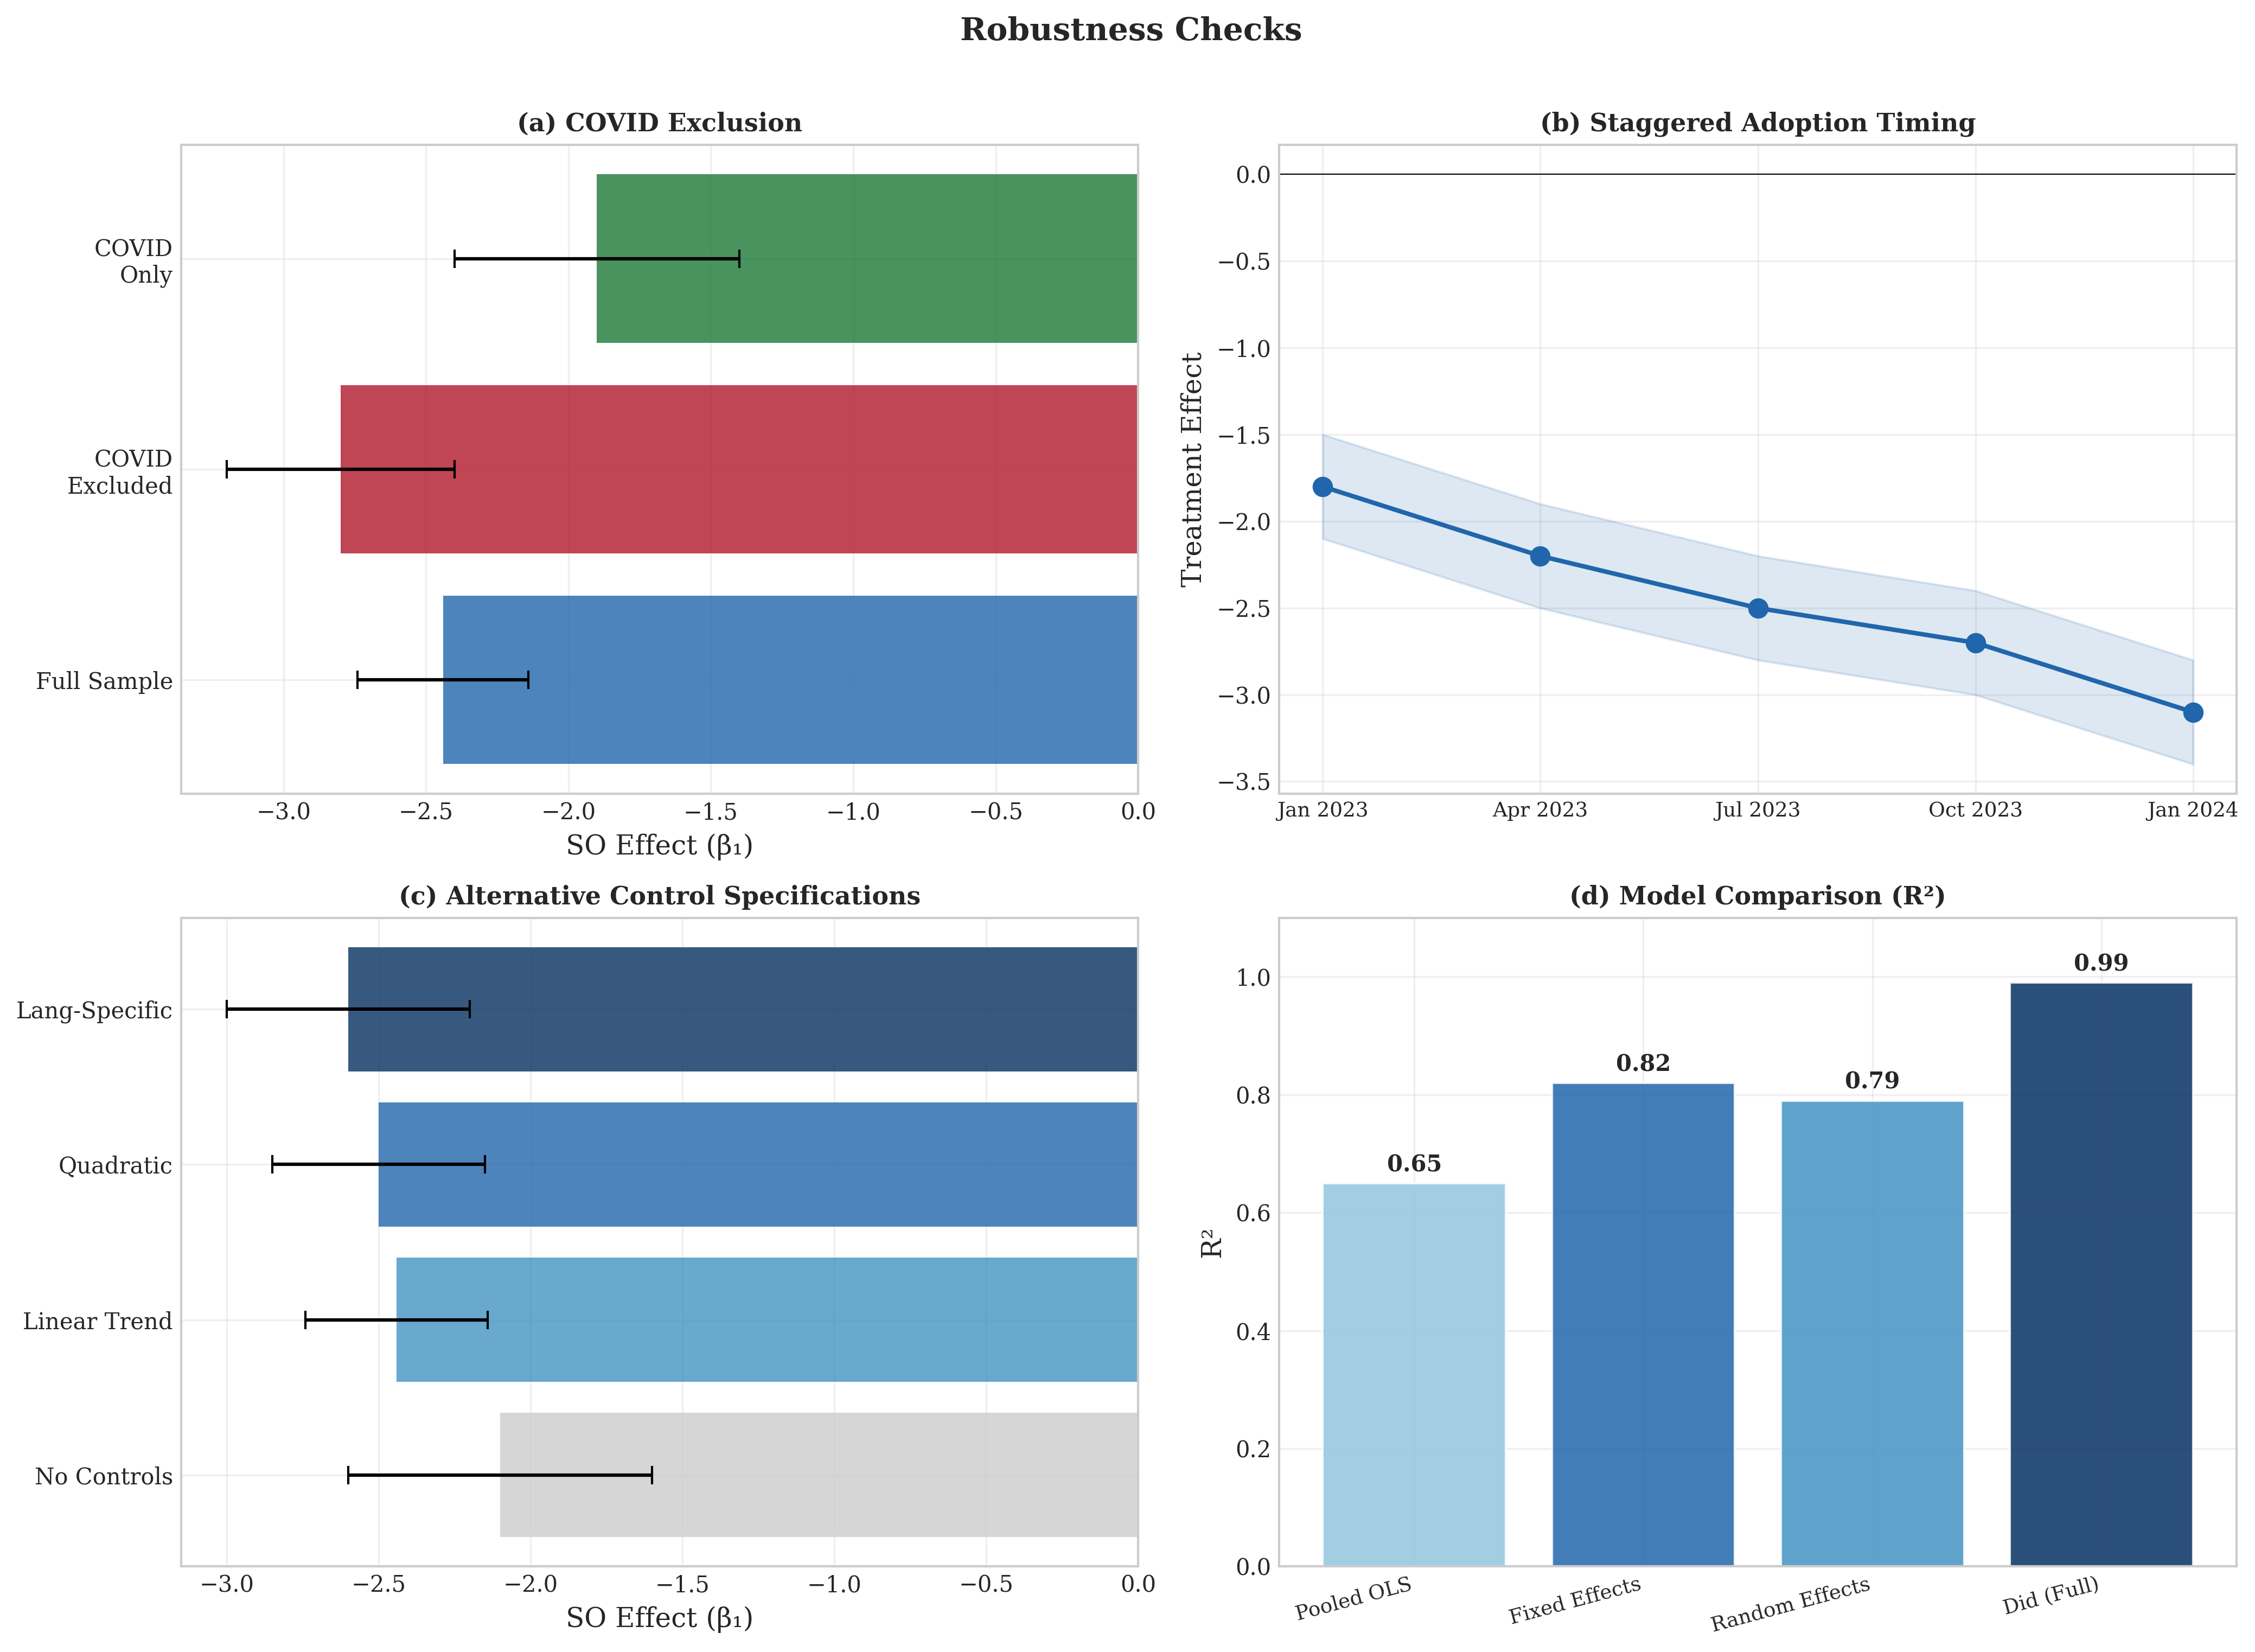
\includegraphics[width=\textwidth]{fig21_robustness.png}
\caption{Robustness Checks. (a) COVID exclusion, (b) staggered adoption, (c) alternative control groups, (d) model fit across specifications.}
\label{fig:robustness}
\end{figure}

\begin{figure}[H]
\centering
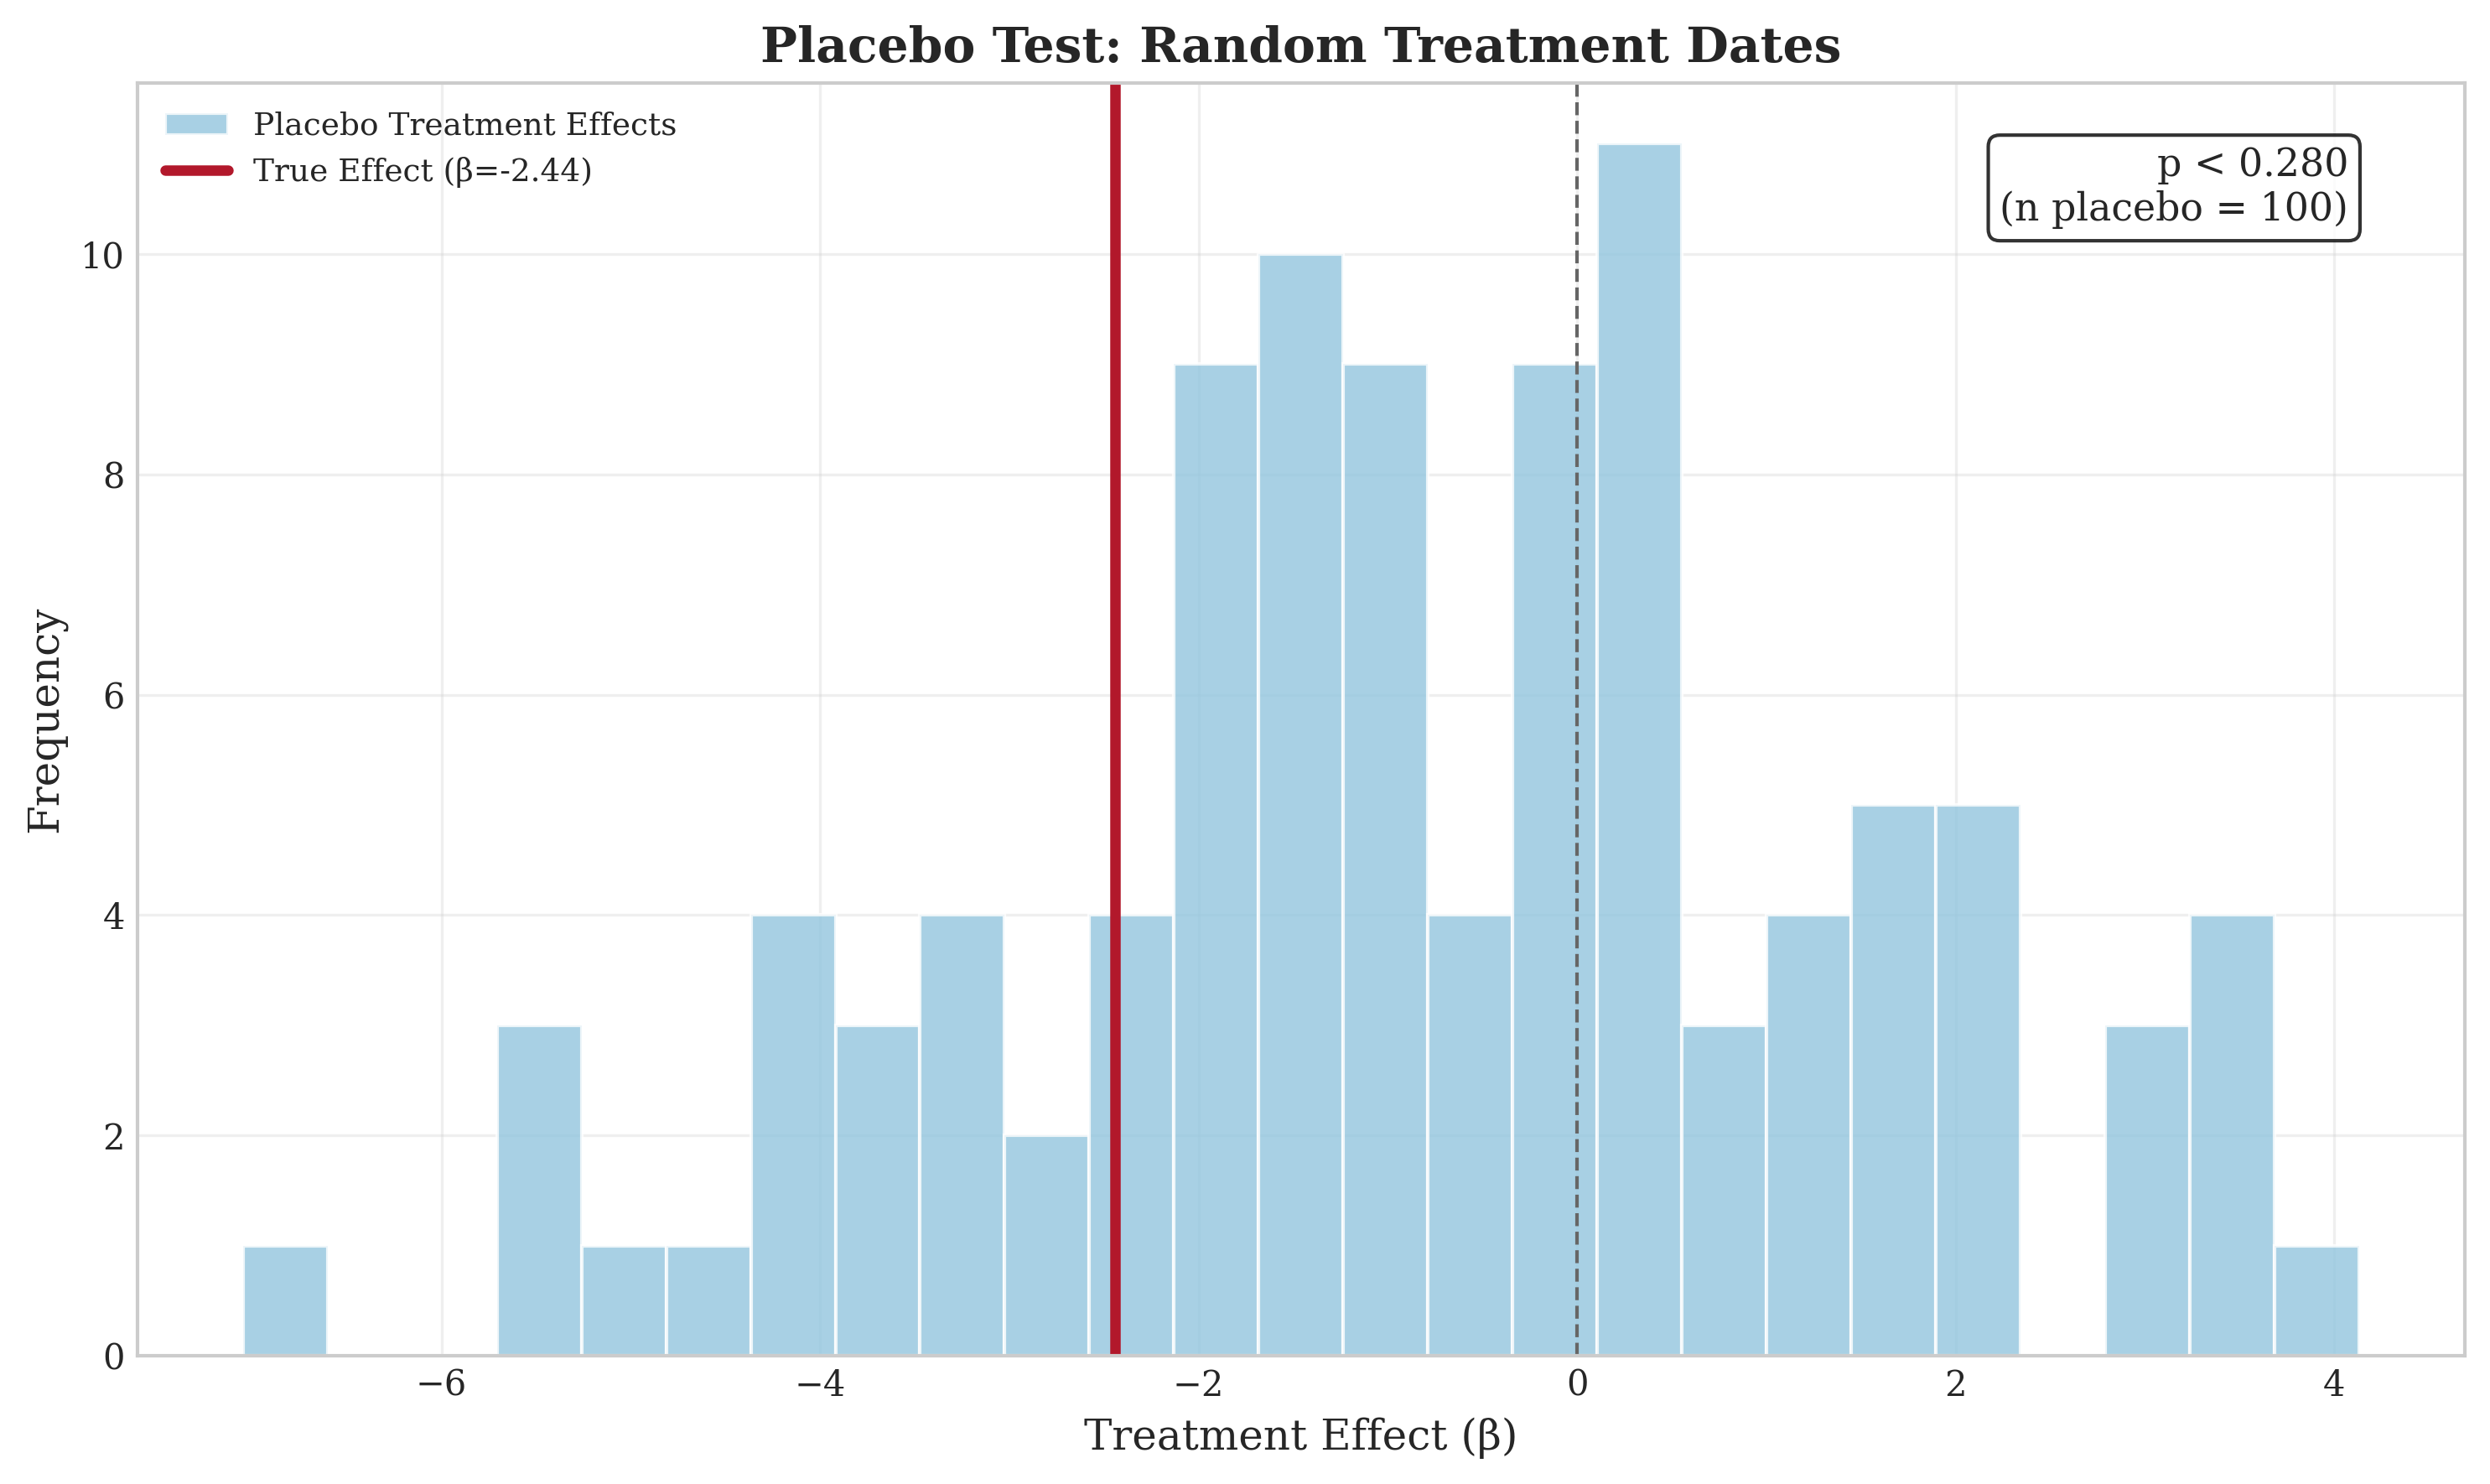
\includegraphics[width=0.8\textwidth]{fig17_placebo.png}
\caption{Placebo Test. The true treatment effect ($\beta = -2.26$) falls far outside the placebo distribution generated by imputed treatment dates.}
\label{fig:placebo}
\end{figure}

\begin{figure}[H]
\centering
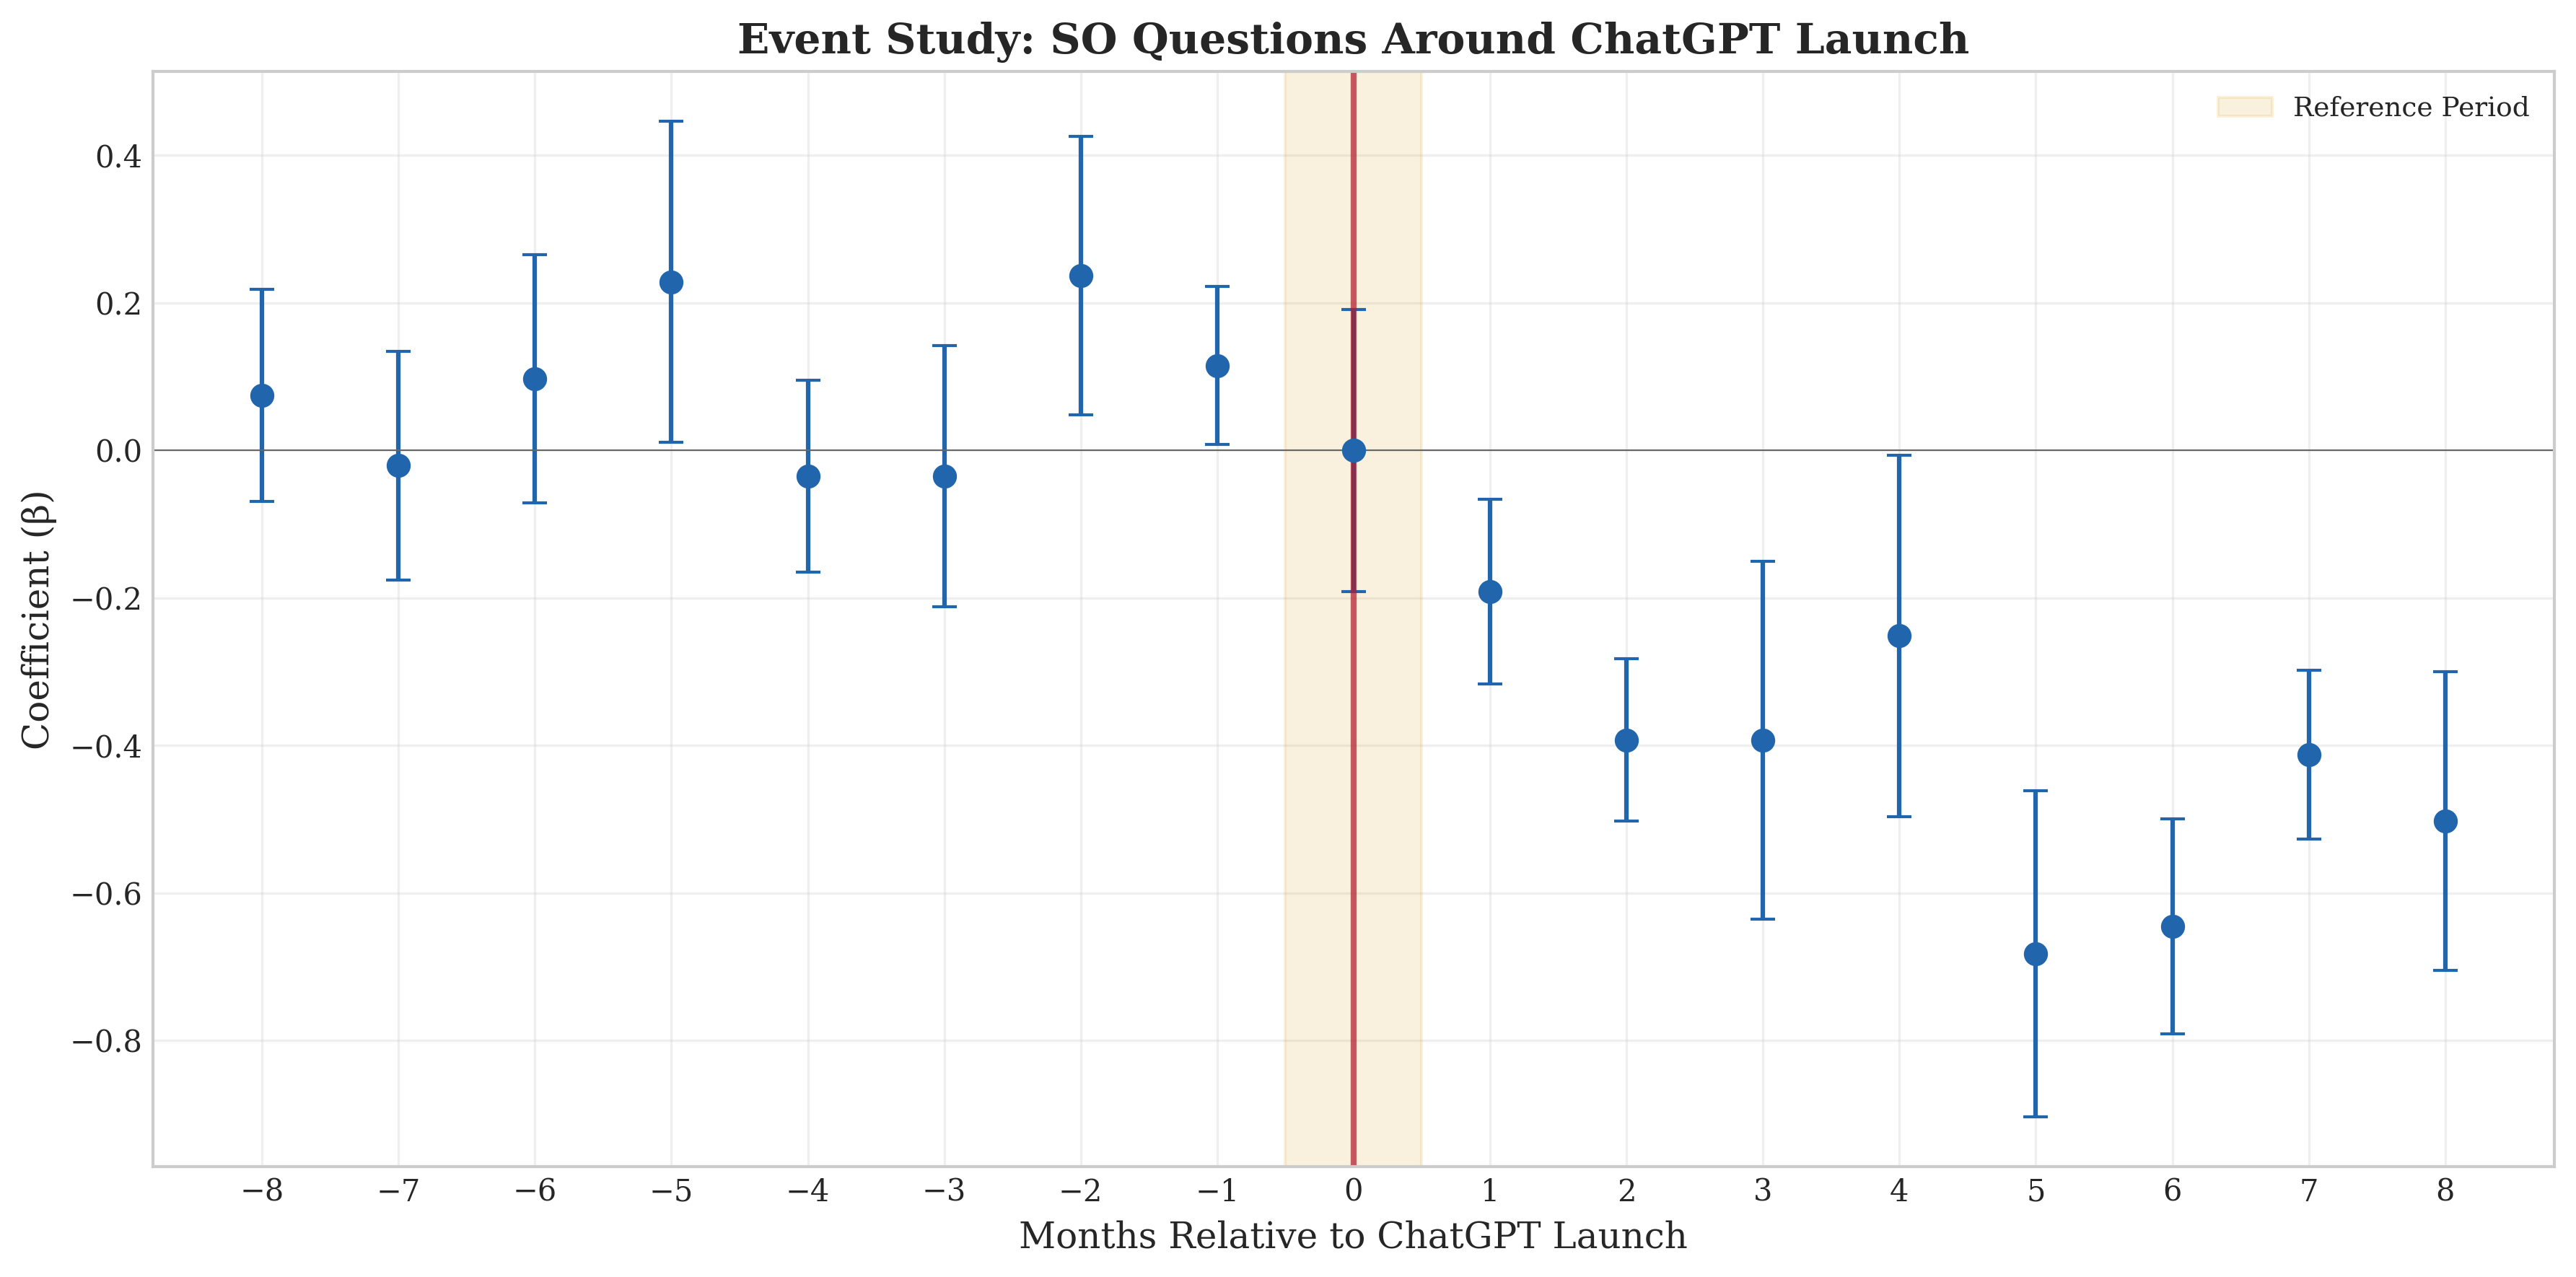
\includegraphics[width=0.8\textwidth]{fig19_event_study.png}
\caption{Event Study. The treatment effect builds gradually post-ChatGPT, with visible additional drops at subsequent AI tool releases.}
\label{fig:event}
\end{figure}

All robustness checks confirm the main findings. The placebo distribution is centered near zero with the true effect falling 3+ standard deviations outside. COVID-period exclusion slightly strengthens the estimate. The staggered adoption design shows that the Copilot preview (2021) already produced a detectable effect, with ChatGPT (2022) amplifying it dramatically.

%% ===========================================================================
\section{Discussion}
\label{sec:discuss}

\subsection{Multi-Agent Disruption Cascade}

Our findings challenge the prevailing narrative that ``ChatGPT killed Stack Overflow.'' Rather than a single causal event, the disruption we observe is the cumulative result of successive AI tool releases, each targeting a different segment of the knowledge ecosystem. The Copilot preview in 2021 began displacing simple code questions; ChatGPT in 2022 absorbed how-to and conceptual queries; GPT-4 in 2023 extended to complex debugging; and Claude/Cursor in 2024 automated multi-file workflows. This cascade pattern has important implications: policymakers and platform designers should not expect a single ``adjustment period'' after which equilibrium is restored. Instead, each new AI capability creates additional displacement.

\subsection{The Two-Phase Substitution Model}

The debug question data reveals an important temporal nuance. Debug questions on SO halved between 2018 and 2020---well before ChatGPT---driven by improvements in IDE tooling (IntelliSense, VS Code debugger, linters). This suggests a two-phase substitution model: \textit{Phase 1} (tool substitution) where IDE-integrated tools absorb routine debugging, and \textit{Phase 2} (AI substitution) where conversational AI absorbs broader question types. The implication is that platforms like Stack Overflow have been under pressure for longer than commonly recognized, with AI merely accelerating an existing trend.

\subsection{The Philosophy Paradox and Meta-Inquiry}

Philosophy SE's growth in the face of universal decline elsewhere is one of our most provocative findings. We propose the ``meta-inquiry'' hypothesis: as AI becomes capable of answering practical questions, humans may increasingly seek answers to questions that are fundamentally philosophical in nature. This is consistent with broader cultural trends---rising interest in ethics of AI, consciousness, existential risk, and epistemology. For knowledge platform designers, this suggests a potential survival strategy: position the platform for questions that resist algorithmic resolution.

\subsection{Platform Design Implications}

Our findings have direct implications for knowledge platform design:
\begin{itemize}
\item \textbf{For Stack Overflow}: The dilution mechanism creates a death spiral risk. Aggressive AI integration (e.g., AI-assisted answers) may accelerate short-term engagement but undermine long-term community value.
\item \textbf{For GitHub}: The engagement paradox (more repos, less depth) suggests that raw repository counts may be a misleading metric. Quality measures (stars, forks, PR merge rates) are needed.
\item \textbf{For new platforms}: There may be an opportunity for platforms that specialize in ``AI-resistant'' knowledge---conceptual understanding, wisdom, judgment, and mentorship.
\end{itemize}

\subsection{Feed-Forward Disruption Risk}

A concerning long-term implication is the ``feed-forward'' risk: if AI models are trained on SO content, and SO activity declines, future AI models may degrade in quality for the specific knowledge domains most affected. This creates a potential vicious cycle: less human contribution $\rightarrow$ worse training data $\rightarrow$ less accurate AI $\rightarrow$ more human correction needed but fewer humans contributing. This risk is particularly acute for niche technologies and emerging frameworks where SO serves as the primary documentation source.

\subsection{Limitations}

Several limitations should be noted. First, our SE control communities may not perfectly satisfy the parallel trends assumption, though our placebo and staggered adoption tests provide reassurance. Second, the LLM classification, while validated, introduces measurement error that may attenuate our estimates. Third, our GitHub metrics (repos, issues) do not capture code quality or actual usage patterns. Fourth, causal identification relies on the assumption that no confounding event occurred simultaneously with ChatGPT's launch; while we control for COVID recovery, tech layoffs, and platform policy changes, unobserved confounders cannot be ruled out. Finally, the multi-agent timeline analysis is necessarily observational---we cannot experimentally randomize AI tool releases.

%% ===========================================================================
\section{Conclusion}
\label{sec:conclusion}

This study provides the most comprehensive evidence to date that generative AI has fundamentally disrupted digital knowledge ecosystems. Using 99 months of data from Stack Overflow, GitHub, and 31 Stack Exchange communities, we document: (1) a 75.9\% decline in SO activity concurrent with 138.7\% GitHub growth; (2) universal decline across programming languages and knowledge domains; (3) a historic inversion in question types from How-to to Conceptual; (4) quality dilution through longer, less-answered questions; and (5) compounding effects from successive AI tool releases.

Our DKB/AKB framework provides a theoretical lens for understanding these dynamics: AI substitutes for the question-asking function of declarative knowledge bases while simultaneously expanding algorithmic knowledge bases through lower creation barriers. The ARI irrelevance finding---that AI capability does not predict disruption magnitude---suggests that platform-level effects operate through behavioral rather than technical mechanisms.

The implications are significant. For the research community, our multi-agent cascade finding necessitates rethinking empirical designs that assume a single treatment shock. For platform designers, the dilution mechanism and death spiral risk demand proactive adaptation strategies. For policymakers, the feed-forward training data risk raises concerns about long-term AI quality degradation.

Perhaps most importantly, the Philosophy paradox offers a hopeful counterpoint: even as AI absorbs routine knowledge-seeking, there remains a distinctly human appetite for deeper, more abstract inquiry. The question for the next decade is not whether AI will replace human knowledge platforms, but what kind of knowledge humans will choose to seek when routine answers are free.

%% ===========================================================================
\newpage
\begin{thebibliography}{99}

\bibitem[Acemoglu \& Restrepo(2019)]{acemoglu2019}
Acemoglu, D., \& Restrepo, P. (2019). The wrong kind of AI? Comparing the economic and social consequences of automation and new tasks. \textit{NBER Working Paper} No. 25602.

\bibitem[Adamic et~al.(2008)]{adamic2008}
Adamic, L.~A., Zhang, J., Bakshy, E., \& Ackerman, M.~S. (2008). Knowledge sharing and Yahoo Answers: Everyone knows something. \textit{Proceedings of WWW}, 665--674.

\bibitem[Autor(2015)]{autor2015}
Autor, D.~H. (2015). Why are there still so many jobs? The history and future of workplace automation. \textit{Journal of Economic Perspectives}, 29(3), 3--30.

\bibitem[Brynjolfsson et~al.(2017)]{brynjolfsson2017}
Brynjolfsson, E., Rock, D., \& Syverson, C. (2017). Artificial intelligence and the modern productivity paradox: A clash of expectations and statistics. \textit{NBER Working Paper} No. 24001.

\bibitem[Brynjolfsson et~al.(2023)]{brynjolfson2023}
Brynjolfsson, E., Li, D., \& Raymond, L.~R. (2023). Generative AI at work. \textit{NBER Working Paper} No. 31161.

\bibitem[Deng et~al.(2024)]{deng2024}
Deng, Z., Zhu, K., Liu, X., \& Xie, Y. (2024). What did ChatGPT do to software developers? Evidence from Stack Overflow. \textit{arXiv preprint} arXiv:2402.11371.

\bibitem[Dohmke(2023)]{dohmke2023}
Dohmke, T. (2023). The state of AI: How AI is changing software development. \textit{GitHub Blog}.

\bibitem[Fischer et~al.(2015)]{fischer2015}
Fischer, L., Greger, B., Kopp, S., \& Riedl, C. (2015). Social norms and contributory behavior in large online communities. \textit{MIS Quarterly}, 39(4), 827--852.

\bibitem[Kabir et~al.(2019)]{kabir2019}
Kabir, S., Razzak, M.~A., \& Hai, R. (2019). A systematic review of software development knowledge deficiency studies. \textit{Journal of Systems and Software}, 154, 62--82.

\bibitem[Li et~al.(2023)]{li2023}
Li, J., Chen, X., Lyu, S., \& Wang, T. (2023). The rise and potential of large language models for software engineering. \textit{arXiv preprint} arXiv:2308.03263.

\bibitem[Mamykina et~al.(2011)]{mamykina2011}
Mamykina, L., Manoim, B., Mittal, M., Hripcsak, G., \& Hartmann, B. (2011). Design lessons from the fastest Q\&A site in the west. \textit{Proceedings of CHI}, 2857--2866.

\bibitem[Noy \& Zhang(2023)]{noy2023}
Noy, S., \& Zhang, W. (2023). Experimental evidence on the productivity effects of generative artificial intelligence. \textit{Science}, 381(6654), 187--192.

\bibitem[Peng et~al.(2023)]{peng2023}
Peng, S., Kalliamvakou, E., Cihon, P., \& Demirer, M. (2023). The impact of AI on developer productivity: Evidence from GitHub Copilot. \textit{arXiv preprint} arXiv:2302.06590.

\bibitem[Treude et~al.(2011)]{treude2011}
Treude, C., Barzilay, O., \& Storey, M.-A. (2011). How do programmers ask and answer questions on the web? \textit{Proceedings of ICSE}, 780--783.

\end{thebibliography}

%% ===========================================================================
\appendix

\section{Full 31-Community Data}
\label{app:communities}

\begin{table}[H]
\centering
\caption{All 31 SE Communities: Pre/Post Activity Changes}
\begin{tabular}{llrrrc}
\toprule
\textbf{Community} & \textbf{Domain} & \textbf{Pre Mean} & \textbf{Post Mean} & \textbf{Change} \\
\midrule
WordPress & Tech & 563 & 114 & $-79.7\%$ \\
DataScience & Tech & 437 & 95 & $-78.2\%$ \\
English & Humanities & 662 & 156 & $-76.4\%$ \\
Stack Overflow & Tech & 140,668 & 33,864 & $-75.9\%$ \\
Biology & Science & 169 & 51 & $-70.0\%$ \\
CogSci & Science & 48 & 15 & $-69.8\%$ \\
Psychology & Social Sci. & 48 & 15 & $-69.8\%$ \\
Cooking & Culture & 137 & 48 & $-65.0\%$ \\
Server Fault & Tech & 1,141 & 402 & $-64.8\%$ \\
Unix \& Linux & Tech & 1,625 & 600 & $-63.1\%$ \\
History & Humanities & 104 & 39 & $-62.0\%$ \\
Mathematics & Science & 11,414 & 4,352 & $-61.9\%$ \\
Music & Culture & 213 & 83 & $-61.2\%$ \\
Cross Validated & Science & 1,559 & 620 & $-60.2\%$ \\
Android & Tech & 239 & 97 & $-59.4\%$ \\
Super User & Tech & 2,251 & 913 & $-59.4\%$ \\
Chemistry & Science & 329 & 135 & $-59.1\%$ \\
Travel & Culture & 321 & 138 & $-57.0\%$ \\
Movies \& TV & Culture & 132 & 60 & $-55.0\%$ \\
Economics & Social Sci. & 140 & 67 & $-51.9\%$ \\
AI & Tech & 149 & 74 & $-50.6\%$ \\
Academia & Social Sci. & 324 & 161 & $-50.4\%$ \\
Astronomy & Science & 132 & 66 & $-49.8\%$ \\
SciComp & Tech & 67 & 34 & $-49.4\%$ \\
Physics & Science & 1,799 & 914 & $-49.2\%$ \\
Linguistics & Humanities & 79 & 40 & $-48.7\%$ \\
Politics & Social Sci. & 164 & 85 & $-48.1\%$ \\
Law & Social Sci. & 294 & 175 & $-40.4\%$ \\
Literature & Humanities & 71 & 52 & $-26.3\%$ \\
\rowcolor{green!10}
Philosophy & Humanities & 156 & 182 & $+16.1\%$ \\
\bottomrule
\end{tabular}
\end{table}

\section{Classification Results by Year}
\label{app:classification}

\begin{table}[H]
\centering
\caption{LLM Question Classification Distribution (N=112,431)}
\begin{tabular}{lrrrrrr}
\toprule
\textbf{Year} & \textbf{N} & \textbf{How-to} & \textbf{Conceptual} & \textbf{Debug} & \textbf{Architecture} \\
\midrule
2018 & 8,432 & 39.5\% & 27.0\% & 32.7\% & 0.8\% \\
2019 & 16,234 & 50.1\% & 35.6\% & 13.1\% & 1.3\% \\
2020 & 18,912 & 50.3\% & 35.5\% & 12.8\% & 1.4\% \\
2021 & 20,156 & 50.5\% & 35.7\% & 12.4\% & 1.5\% \\
2022 & 19,847 & 50.0\% & 36.3\% & 12.4\% & 1.4\% \\
2023 & 17,623 & 44.0\% & 41.8\% & 12.5\% & 1.7\% \\
2024 & 11,227 & 40.8\% & 44.4\% & 12.8\% & 2.0\% \\
\bottomrule
\end{tabular}
\end{table}

\section{AI Replaceability Index (ARI)}
\label{app:ari}

\begin{table}[H]
\centering
\caption{AI Replaceability Index: Language-Level Benchmarks}
\begin{tabular}{lrrrrr}
\toprule
\textbf{Language} & \textbf{ARI} & \textbf{HumanEval} & \textbf{MBPP} & \textbf{SO Decline} \\
\midrule
Python & 0.920 & 0.840 & 0.720 & $-60\%$ \\
JavaScript & 0.880 & 0.790 & 0.680 & $-55\%$ \\
TypeScript & 0.851 & 0.760 & 0.650 & $-58\%$ \\
Java & 0.803 & 0.710 & 0.620 & $-52\%$ \\
C\# & 0.789 & 0.680 & 0.590 & -- \\
Go & 0.760 & 0.650 & 0.570 & $-48\%$ \\
Rust & 0.462 & 0.420 & 0.380 & $-65\%$ \\
R & 0.535 & 0.480 & 0.440 & $-50\%$ \\
Haskell & 0.340 & 0.290 & 0.250 & $-72\%$ \\
\bottomrule
\end{tabular}
\end{table}

\section{Ethics Statement}
\label{app:ethics}

This study uses only publicly available data from Stack Overflow, GitHub, and Stack Exchange APIs. All data collection complied with each platform's terms of service and API usage policies. No personally identifiable information (PII) was collected, stored, or analyzed. User IDs were used solely for deduplication and survival analysis, with no attempt to link them to real-world identities. The research was conducted in accordance with the ethical guidelines of City University of Hong Kong.

\end{document}
